\documentclass[a4paper,12pt,leqno]{article}
\usepackage{titling}
\newcommand{\subtitle}[1]{%
  \posttitle{%
    \par\end{center}
    \begin{center}\large#1\end{center}
    \vskip0.5em}%
}

\usepackage{algorithmic}
\usepackage{multirow}
\usepackage{float}
\usepackage[table]{xcolor}
\usepackage{graphicx}
\usepackage{booktabs}
\usepackage{threeparttable}
\usepackage{lscape}
\usepackage{subfigure}
\usepackage{parskip}
\usepackage{natbib}
\usepackage{hyperref}
\usepackage{rotating}
\usepackage{ltablex}
\usepackage{breakurl}
\usepackage{ifthen}
\usepackage{xstring}
%\usepackage[dvipsnames]{xcolor}
\usepackage[margin = 0.5in]{geometry}
\usepackage[ut f8]{inputenc}
\usepackage{array}
\floatstyle{ruled}
\restylefloat{table}
\restylefloat{figure}
\newcommand{\floatintro}[1]{
  \vspace*{0.1in}
  {\footnotesize
    #1
  }
  \vspace*{0.1in}
}
\makeatletter    
\if@compatibility
\renewenvironment{titlepage}
{%
  \cleardoublepage
  \if@twocolumn
  \@restonecoltrue\onecolumn
  \else
  \@restonecolfalse\newpage
  \fi
  \thispagestyle{empty}%
  % \setcounter{page}\z@
}%
{\if@restonecol\twocolumn \else \newpage \fi
}
\else
\renewenvironment{titlepage}
{%
  \cleardoublepage
  \if@twocolumn
  \@restonecoltrue\onecolumn
  \else
  \@restonecolfalse\newpage
  \fi
  \thispagestyle{empty}%
  % \setcounter{page}\@ne
}%
{\if@restonecol\twocolumn \else \newpage \fi
  \if@twoside\else
  % \setcounter{page}\@ne
  \fi
}
\fi
\makeatother

\newlength{\textwidthorig}
\setlength{\textwidthorig}{\textwidth}
\renewcommand{\baselinestretch}{1.1}

% \newcommand{\fullpage}[1]{
%   \part{#1}
%   \begin{minipage}                                                                                                                        
%     \partpage
%   \end{minipage}
% }




\title{Financial reforms metric}
\subtitle{}
\author{Finance research group, IGIDR}

\date{}

\newcolumntype{A}{>{\raggedright\let\newline\\\arraybackslash\hspace{0pt}}p{2cm}}
\newcolumntype{B}{>{\raggedright\let\newline\\\arraybackslash\hspace{0pt}}p{2.5cm}}
\newcolumntype{C}{>{\raggedright\let\newline\\\arraybackslash\hspace{0pt}}p{4cm}}
\newcolumntype{D}{>{\raggedright\let\newline\\\arraybackslash\hspace{0pt}}p{6cm}}
\newcolumntype{E}{>{\raggedright\let\newline\\\arraybackslash\hspace{0pt}}p{1.5cm}}
\newcolumntype{F}{>{\center\let\newline\\\arraybackslash\hspace{0pt}}p{5cm}}
\newcolumntype{G}{>{\center\let\newline\\\arraybackslash\hspace{0pt}}p{8.5cm}}
\newcolumntype{H}{>{\center\let\newline\\\arraybackslash\hspace{0pt}}p{5cm}}

\newcommand{\present}{e}
\newcommand{\absent}{n}

\newcommand{\lfgofac}{n}
\newcommand{\lfgofadl}{n}
\newcommand{\lfgofale}{n}
\newcommand{\lfgofali}{n}

\newcommand{\lfleaqjfofac}{n}
\newcommand{\lfleaqjfofadl}{n}
\newcommand{\lfleaqjfofale}{n}
\newcommand{\lfleaqjfofali}{n}

\newcommand{\lfcpc}{n}
\newcommand{\lfcpdl}{n}
\newcommand{\lfcple}{n}
\newcommand{\lfcpli}{n}

\newcommand{\lfmprc}{n}
\newcommand{\lfmprdl}{n}
\newcommand{\lfmprle}{n}
\newcommand{\lfmprli}{n}

\newcommand{\lfdc}{n}
\newcommand{\lfddl}{n}
\newcommand{\lfdle}{n}
\newcommand{\lfdli}{n}

\newcommand{\lfccc}{n}
\newcommand{\lfccdl}{n}
\newcommand{\lfccle}{n}
\newcommand{\lfccli}{n}

\newcommand{\lfrc}{n}
\newcommand{\lfrdl}{n}
\newcommand{\lfrle}{n}
\newcommand{\lfrli}{n}

\newcommand{\lffrac}{n}
\newcommand{\lffradl}{n}
\newcommand{\lffrale}{n}
\newcommand{\lffrali}{n}

\newcommand{\lfrbic}{n}
\newcommand{\lfrbidl}{n}
\newcommand{\lfrbile}{n}
\newcommand{\lfrbili}{n}

\newcommand{\lfufac}{n}
\newcommand{\lfufadl}{n}
\newcommand{\lfufale}{n}
\newcommand{\lfufali}{n}

\newcommand{\lfpdmac}{n}
\newcommand{\lfpdmadl}{n}
\newcommand{\lfpdmale}{n}
\newcommand{\lfpdmali}{n}

\newcommand{\lffsdcc}{n}
\newcommand{\lffsdcdl}{n}
\newcommand{\lffsdcle}{n}
\newcommand{\lffsdcli}{n}

\newcommand{\lf}{n}

\newcommand{\memi}{n}
\newcommand{\meebit}{n}
\newcommand{\mesra}{n}
\newcommand{\meeor}{n}

\newcommand{\mbnmi}{n}
\newcommand{\mbnebit}{n}
\newcommand{\mbnsra}{n}
\newcommand{\mbneor}{n}

\newcommand{\mcmi}{n}
\newcommand{\mcebit}{n}
\newcommand{\mcsra}{n}
\newcommand{\mcsr}{n}
\newcommand{\mceor}{n}


\newcommand{\m}{n}

\makeatletter
\newcommand{\roystreqtest}[2]{%
  \ifnum\pdfstrcmp{#1}{#2}=0
    \expandafter\@firstoftwo
  \else
    \expandafter\@secondoftwo
  \fi
}

\makeatother
\newcommand{\glfgofa}[4]{
  \begin{tabular} {ABCDE}
    \hline
    \noalign{\vskip .09in}
    \multicolumn{5}{p{3.5in}}{\textbf{\small{Legal foundations:}}} \\ \hline
    \noalign{\vskip .06in}
    \multicolumn{5}{p{3.5in}}{\textbf{\textit{\footnotesize{Governance of financial agencies:}}}} \\ \hline
    \noalign{\vskip .01in}
    \roystreqtest{#1}{\present}
    {\multicolumn{3}{c}{\textbf{\underline{\footnotesize{Concepts}}}} & \multicolumn{2}{c}{\textbf{\footnotesize{\colorbox{lightgray}{weight: 5}}}} \\ \hline           
    \noalign{\vskip .06in}
    \textbf{Date} & \textbf{Milestone} & \textbf{URL} & \textbf{Story} & \textbf{Score} \\ \hline
    \input{../TABLES/legal_foundations_governance_of_financial_agencies_concepts.tex}
    \hline
    \noalign{\vskip .06in}
    }{}
    \roystreqtest{#2}{\present}
    {\multicolumn{3}{c}{\textbf{\underline{\footnotesize{Draft Law}}}} & \multicolumn{2}{c}{\textbf{\footnotesize{\colorbox{lightgray}{weight: 5}}}}  \\ \hline
    \noalign{\vskip .01in}
    \textbf{Date} & \textbf{Milestone} & \textbf{URL} & \textbf{Story} & \textbf{Score} \\ \hline
    \input{../TABLES/legal_foundations_governance_of_financial_agencies_draftlaw.tex}
    \hline
    \noalign{\vskip .06in}
    }{}
    \roystreqtest{#3}{\present}
    {\multicolumn{3}{c}{\textbf{\underline{\footnotesize{Law Enacted}}}} & \multicolumn{2}{c}{\textbf{\footnotesize{\colorbox{lightgray}{weight:10}}}}  \\ \hline
    \noalign{\vskip .01in}
    \textbf{Date} & \textbf{Milestone} & \textbf{URL} & \textbf{Story} & \textbf{Score} \\ \hline
    \input{../TABLES/legal_foundations_governance_of_financial_agencies_lawenacted.tex}
    \hline
    \noalign{\vskip .06in}
    }{}
    \roystreqtest{#4}{\present}
    {\multicolumn{3}{c}{\textbf{\underline{\footnotesize{Law Implemented}}}} & \multicolumn{2}{c}{\textbf{\footnotesize{\colorbox{lightgray}{weight:10}}}}  \\ \hline
    \noalign{\vskip .01in}
    \textbf{Date} & \textbf{Milestone} & \textbf{URL} & \textbf{Story} & \textbf{Score} \\ \hline
    \input{../TABLES/legal_foundations_governance_of_financial_agencies_lawimplemented.tex}
    \hline
    \noalign{\vskip .06in}
    }{}
    \multicolumn{5}{p{6in}}{\textit{\scriptsize{Explanation:
    Legal foundations for working of the board, report, appointments.}}}
  \end{tabular}
}

\newcommand{\glfleaqjfofa}[4]{%
  \begin{tabular} {ABCDE}%{p{1.5cm}p{1.5cm}p{5cm}p{5cm}p{1cm}}
    \hline
    \noalign{\vskip .09in}
    \multicolumn{5}{p{7in}}{\textbf{\small{Legal foundations:}}} \\ \hline
    \noalign{\vskip .06in}
    \multicolumn{5}{p{7in}}{\textbf{\textit{\footnotesize{Legislative, executive and quasi judicial functions of financial agencies:}}}} \\ \hline
    \noalign{\vskip .01in}
    \roystreqtest{#1}{\present}
    {\multicolumn{3}{c}{\textbf{\underline{\footnotesize{Concepts}}}} & \multicolumn{2}{c}{\textbf{\footnotesize{\colorbox{lightgray}{weight: 5}}}}  \\ \hline           
    \noalign{\vskip .06in}
    \textbf{Date} & \textbf{Milestone} & \textbf{URL} & \textbf{Story} & \textbf{Score} \\ \hline
    \input{../TABLES/legal_foundations_legislative_executive_and_quasi-judicial_functions_of_financial_agencies_concepts.tex}
    \hline
    \noalign{\vskip .06in}
    }{}
    \roystreqtest{#2}{\present}
    {\multicolumn{3}{c}{\textbf{\underline{\footnotesize{Draft Law}}}} & \multicolumn{2}{c}{\textbf{\footnotesize{\colorbox{lightgray}{weight: 5}}}}  \\ \hline
    \noalign{\vskip .01in}
    \textbf{Date} & \textbf{Milestone} & \textbf{URL} & \textbf{Story} & \textbf{Score} \\ \hline
    \input{../TABLES/legal_foundations_legislative_executive_and_quasi-judicial_functions_of_financial_agencies_draftlaw.tex}
    \hline
    \noalign{\vskip .06in}
    }{}
    \roystreqtest{#3}{\present}
    {\multicolumn{3}{c}{\textbf{\underline{\footnotesize{Law Enacted}}}} & \multicolumn{2}{c}{\textbf{\footnotesize{\colorbox{lightgray}{weight:10}}}}  \\ \hline
    \noalign{\vskip .01in}
    \textbf{Date} & \textbf{Milestone} & \textbf{URL} & \textbf{Story} & \textbf{Score} \\ \hline
    \input{../TABLES/legal_foundations_legislative_executive_and_quasi-judicial_functions_of_financial_agencies_lawenacted.tex}
    \hline
    \noalign{\vskip .06in}
    }{}
    \roystreqtest{#4}{\present}
    {\multicolumn{3}{c}{\textbf{\underline{\footnotesize{Law Implemented}}}} & \multicolumn{2}{c}{\textbf{\footnotesize{\colorbox{lightgray}{weight:10}}}}  \\ \hline
    \noalign{\vskip .01in}
    \textbf{Date} & \textbf{Milestone} & \textbf{URL} & \textbf{Story} & \textbf{Score} \\ \hline
    \input{../TABLES/legal_foundations_legislative_executive_and_quasi-judicial_functions_of_financial_agencies_lawimplemented.tex}
    \hline
    \noalign{\vskip .06in}
    \hline
    
    }{}
    \multicolumn{5}{p{6in}}{\textit{\scriptsize{Explanation:
    Establish procedural law for how financial agencies will perform
    their legislative, executive and quasi-judicial functions.}}}
  \end{tabular}
}


\newcommand{\glfcp}[4]{%
  \begin{tabular} {ABCDE}%{p{1.5cm}p{1.5cm}p{5cm}p{5cm}p{1cm}}
    \hline
    \noalign{\vskip .09in}
    \multicolumn{5}{p{7in}}{\textbf{\small{Legal foundations:}}} \\ \hline
    \noalign{\vskip .06in}
    \multicolumn{5}{p{7in}}{\textbf{\textit{\footnotesize{Consumer protection:}}}} \\ \hline
    \noalign{\vskip .01in}
    \roystreqtest{#1}{\present}
    {\multicolumn{3}{c}{\textbf{\underline{\footnotesize{Concepts}}}} & \multicolumn{2}{c}{\textbf{\footnotesize{\colorbox{lightgray}{weight: 5}}}}  \\ \hline           
    \noalign{\vskip .06in}
    \textbf{Date} & \textbf{Milestone} & \textbf{URL} & \textbf{Story} & \textbf{Score} \\ \hline
    \input{../TABLES/legal_foundations_consumer_protection_concepts.tex}
    \hline
    \noalign{\vskip .06in}
    }{}
    \roystreqtest{#2}{\present}
    {\multicolumn{3}{c}{\textbf{\underline{\footnotesize{Draft Law}}}} & \multicolumn{2}{c}{\textbf{\footnotesize{\colorbox{lightgray}{weight: 5}}}}  \\ \hline
    \noalign{\vskip .01in}
    \textbf{Date} & \textbf{Milestone} & \textbf{URL} & \textbf{Story} & \textbf{Score} \\ \hline
    \input{../TABLES/legal_foundations_consumer_protection_draftlaw.tex}
    \hline
    \noalign{\vskip .06in}
    }{}
    \roystreqtest{#3}{\present}
    {\multicolumn{3}{c}{\textbf{\underline{\footnotesize{Law Enacted}}}} & \multicolumn{2}{c}{\textbf{\footnotesize{\colorbox{lightgray}{weight:10}}}}  \\ \hline
    \noalign{\vskip .01in}
    \textbf{Date} & \textbf{Milestone} & \textbf{URL} & \textbf{Story} & \textbf{Score} \\ \hline
    \input{../TABLES/legal_foundations_consumer_protection_lawenacted.tex}
    \hline
    \noalign{\vskip .06in}
    }{}
    \roystreqtest{#4}{\present}
    {\multicolumn{3}{c}{\textbf{\underline{\footnotesize{Law Implemented}}}} & \multicolumn{2}{c}{\textbf{\footnotesize{\colorbox{lightgray}{weight:10}}}}  \\ \hline
    \noalign{\vskip .01in}
    \textbf{Date} & \textbf{Milestone} & \textbf{URL} & \textbf{Story} & \textbf{Score} \\ \hline
    \input{../TABLES/legal_foundations_consumer_protection_lawimplemented.tex}
    \hline
    \noalign{\vskip .06in}
    }{}
    \multicolumn{5}{p{6in}}{\textit{\scriptsize{Explanation:
    Law that establishes rights of consumers of financial products and
    services.}}}
  \end{tabular}
}

\newcommand{\glfmpr}[4]{%
  \begin{tabular} {ABCDE}%{p{1.5cm}p{1.5cm}p{5cm}p{5cm}p{1cm}}
    \hline
    \noalign{\vskip .09in}
    \multicolumn{5}{p{7in}}{\textbf{\small{Legal foundations:}}} \\ \hline
    \noalign{\vskip .06in}
    \multicolumn{5}{p{7in}}{\textbf{\textit{\footnotesize{Micro-prudential
    regulations:}}}} \\ \hline
    \noalign{\vskip .01in}
    \roystreqtest{#1}{\present}
    {\multicolumn{3}{c}{\textbf{\underline{\footnotesize{Concepts}}}} & \multicolumn{2}{c}{\textbf{\footnotesize{\colorbox{lightgray}{weight: 5}}}}  \\ \hline           
    \noalign{\vskip .06in}
    \textbf{Date} & \textbf{Milestone} & \textbf{URL} & \textbf{Story} & \textbf{Score} \\ \hline
    \input{../TABLES/legal_foundations_micro-prudential_regulation_concepts.tex}
    \hline
    \noalign{\vskip .06in}
    }{}
    \roystreqtest{#2}{\present}
    {\multicolumn{3}{c}{\textbf{\underline{\footnotesize{Draft Law}}}} & \multicolumn{2}{c}{\textbf{\footnotesize{\colorbox{lightgray}{weight: 5}}}}  \\ \hline
    \noalign{\vskip .01in}
    \textbf{Date} & \textbf{Milestone} & \textbf{URL} & \textbf{Story} & \textbf{Score} \\ \hline
    \input{../TABLES/legal_foundations_micro-prudential_regulation_draftlaw.tex}
    \hline
    \noalign{\vskip .06in}
    }{}
    \roystreqtest{#3}{\present}
    {\multicolumn{3}{c}{\textbf{\underline{\footnotesize{Law Enacted}}}} & \multicolumn{2}{c}{\textbf{\footnotesize{\colorbox{lightgray}{weight:10}}}}  \\ \hline
    \noalign{\vskip .01in}
    \textbf{Date} & \textbf{Milestone} & \textbf{URL} & \textbf{Story} & \textbf{Score} \\ \hline
    \input{../TABLES/legal_foundations_micro-prudential_regulation_lawenacted.tex}
    \hline
    \noalign{\vskip .06in}
    }{}
    \roystreqtest{#4}{\present}
    {\multicolumn{3}{c}{\textbf{\underline{\footnotesize{Law Implemented}}}} & \multicolumn{2}{c}{\textbf{\footnotesize{\colorbox{lightgray}{weight:10}}}}  \\ \hline
    \noalign{\vskip .01in}
    \textbf{Date} & \textbf{Milestone} & \textbf{URL} & \textbf{Story} & \textbf{Score} \\ \hline
    \input{../TABLES/legal_foundations_micro-prudential_regulation_lawimplemented.tex}
    \hline
    \noalign{\vskip .06in}
    }{}
    \multicolumn{5}{p{6in}}{\textit{\scriptsize{Explanation:
    Law that establishes a non-sectoral principles based framework for
    micro-prudential regulation.}}}
  \end{tabular}
}


\newcommand{\glfd}[4]{%
  \begin{tabular} {ABCDE}%{p{1.5cm}p{1.5cm}p{5cm}p{5cm}p{1cm}}
    \hline
    \noalign{\vskip .09in}
    \multicolumn{5}{p{7in}}{\textbf{\small{Legal foundations:}}} \\ \hline
    \noalign{\vskip .06in}
    \multicolumn{5}{p{7in}}{\textbf{\textit{\footnotesize{Development:}}}} \\ \hline
    \noalign{\vskip .01in}
    \roystreqtest{#1}{\present}
    {\multicolumn{3}{c}{\textbf{\underline{\footnotesize{Concepts}}}} & \multicolumn{2}{c}{\textbf{\footnotesize{\colorbox{lightgray}{weight: 5}}}}  \\ \hline           
    \noalign{\vskip .06in}
    \textbf{Date} & \textbf{Milestone} & \textbf{URL} & \textbf{Story} & \textbf{Score} \\ \hline
    \input{../TABLES/legal_foundations_development_concepts.tex}
    \hline
    \noalign{\vskip .06in}
    }{}
    \roystreqtest{#2}{\present}
    {\multicolumn{3}{c}{\textbf{\underline{\footnotesize{Draft Law}}}} & \multicolumn{2}{c}{\textbf{\footnotesize{\colorbox{lightgray}{weight: 5}}}}  \\ \hline
    \noalign{\vskip .01in}
    \textbf{Date} & \textbf{Milestone} & \textbf{URL} & \textbf{Story} & \textbf{Score} \\ \hline
    \input{../TABLES/legal_foundations_development_draftlaw.tex}
    \hline
    \noalign{\vskip .06in}
    }{}
    \roystreqtest{#3}{\present}
    {\multicolumn{3}{c}{\textbf{\underline{\footnotesize{Law Enacted}}}} & \multicolumn{2}{c}{\textbf{\footnotesize{\colorbox{lightgray}{weight:10}}}}  \\ \hline
    \noalign{\vskip .01in}
    \textbf{Date} & \textbf{Milestone} & \textbf{URL} & \textbf{Story} & \textbf{Score} \\ \hline
    \input{../TABLES/legal_foundations_development_lawenacted.tex}
    \hline
    \noalign{\vskip .06in}
    }{}
    \roystreqtest{#4}{\present}
    {\multicolumn{3}{c}{\textbf{\underline{\footnotesize{Law Implemented}}}} & \multicolumn{2}{c}{\textbf{\footnotesize{\colorbox{lightgray}{weight:10}}}}  \\ \hline
    \noalign{\vskip .01in}
    \textbf{Date} & \textbf{Milestone} & \textbf{URL} & \textbf{Story} & \textbf{Score} \\ \hline
    \input{../TABLES/legal_foundations_development_lawimplemented.tex}
    \hline
    \noalign{\vskip .06in}
    }{}
    \multicolumn{5}{p{6in}}{\textit{\scriptsize{Explanation:
    Law that establishes a sound framework for financial development,
    which comprises of improvements in market infrastructure and
    processes and finance for the poor.}}}
  \end{tabular}
}


\newcommand{\glfcc}[4]{%
  \begin{tabular} {ABCDE}%{p{1.5cm}p{1.5cm}p{5cm}p{5cm}p{1cm}}
    \hline
    \noalign{\vskip .09in}
    \multicolumn{5}{p{7in}}{\textbf{\small{Legal foundations:}}} \\ \hline
    \noalign{\vskip .06in}
    \multicolumn{5}{p{7in}}{\textbf{\textit{\footnotesize{Capital controls:}}}} \\ \hline
    \noalign{\vskip .01in}
    \roystreqtest{#1}{\present}
    {\multicolumn{3}{c}{\textbf{\underline{\footnotesize{Concepts}}}} & \multicolumn{2}{c}{\textbf{\footnotesize{\colorbox{lightgray}{weight: 5}}}}  \\ \hline           
    \noalign{\vskip .06in}
    \textbf{Date} & \textbf{Milestone} & \textbf{URL} & \textbf{Story} & \textbf{Score} \\ \hline
    \input{../TABLES/legal_foundations_capital_controls_concepts.tex}
    \hline
    \noalign{\vskip .06in}
    }{}
    \roystreqtest{#2}{\present}
    {\multicolumn{3}{c}{\textbf{\underline{\footnotesize{Draft Law}}}} & \multicolumn{2}{c}{\textbf{\footnotesize{\colorbox{lightgray}{weight: 5}}}}  \\ \hline
    \noalign{\vskip .01in}
    \textbf{Date} & \textbf{Milestone} & \textbf{URL} & \textbf{Story} & \textbf{Score} \\ \hline
    \input{../TABLES/legal_foundations_capital_controls_draftlaw.tex}
    \hline
    \noalign{\vskip .06in}
    }{}
    \roystreqtest{#3}{\present}
    {\multicolumn{3}{c}{\textbf{\underline{\footnotesize{Law Enacted}}}} & \multicolumn{2}{c}{\textbf{\footnotesize{\colorbox{lightgray}{weight:10}}}}  \\ \hline
    \noalign{\vskip .01in}
    \textbf{Date} & \textbf{Milestone} & \textbf{URL} & \textbf{Story} & \textbf{Score} \\ \hline
    \input{../TABLES/legal_foundations_capital_controls_lawenacted.tex}
    \hline
    \noalign{\vskip .06in}
    }{}
    \roystreqtest{#4}{\present}
    {\multicolumn{3}{c}{\textbf{\underline{\footnotesize{Law Implemented}}}} & \multicolumn{2}{c}{\textbf{\footnotesize{\colorbox{lightgray}{weight:10}}}}  \\ \hline
    \noalign{\vskip .01in}
    \textbf{Date} & \textbf{Milestone} & \textbf{URL} & \textbf{Story} & \textbf{Score} \\ \hline
    \input{../TABLES/legal_foundations_capital_controls_lawimplemented.tex}
    \hline
    \noalign{\vskip .06in}
    }{}
    \multicolumn{5}{p{6in}}{\textit{\scriptsize{Explanation:
    Law that establishes sound framework for capital controls.}}}
  \end{tabular}
}

\newcommand{\glfr}[4]{%
  \begin{tabular} {ABCDE}%{p{1.5cm}p{1.5cm}p{5cm}p{5cm}p{1cm}}
    \hline
    \noalign{\vskip .09in}
    \multicolumn{5}{p{7in}}{\textbf{\small{Legal foundations:}}} \\ \hline
    \noalign{\vskip .06in}
    \multicolumn{5}{p{7in}}{\textbf{\textit{\footnotesize{Consumer protection:}}}} \\ \hline
    \noalign{\vskip .01in}
    \roystreqtest{#1}{\present}
    {\multicolumn{3}{c}{\textbf{\underline{\footnotesize{Concepts}}}} & \multicolumn{2}{c}{\textbf{\footnotesize{\colorbox{lightgray}{weight: 5}}}}  \\ \hline           
    \noalign{\vskip .06in}
    \textbf{Date} & \textbf{Milestone} & \textbf{URL} & \textbf{Story} & \textbf{Score} \\ \hline
    \input{../TABLES/legal_foundations_resolution_concepts.tex}
    \hline
    \noalign{\vskip .06in}
    }{}
    \roystreqtest{#2}{\present}
    {\multicolumn{3}{c}{\textbf{\underline{\footnotesize{Draft Law}}}} & \multicolumn{2}{c}{\textbf{\footnotesize{\colorbox{lightgray}{weight: 5}}}}  \\ \hline
    \noalign{\vskip .01in}
    \textbf{Date} & \textbf{Milestone} & \textbf{URL} & \textbf{Story} & \textbf{Score} \\ \hline
    \input{../TABLES/legal_foundations_resolution_draftlaw.tex}
    \hline
    \noalign{\vskip .06in}
    }{}
    \roystreqtest{#3}{\present}
    {\multicolumn{3}{c}{\textbf{\underline{\footnotesize{Law Enacted}}}} & \multicolumn{2}{c}{\textbf{\footnotesize{\colorbox{lightgray}{weight:10}}}}  \\ \hline
    \noalign{\vskip .01in}
    \textbf{Date} & \textbf{Milestone} & \textbf{URL} & \textbf{Story} & \textbf{Score} \\ \hline
    \input{../TABLES/legal_foundations_resolution_lawenacted.tex}
    \hline
    \noalign{\vskip .06in}
    }{}
    \roystreqtest{#4}{\present}
    {\multicolumn{3}{c}{\textbf{\underline{\footnotesize{Law Implemented}}}} & \multicolumn{2}{c}{\textbf{\footnotesize{\colorbox{lightgray}{weight:10}}}}  \\ \hline
    \noalign{\vskip .01in}
    \textbf{Date} & \textbf{Milestone} & \textbf{URL} & \textbf{Story} & \textbf{Score} \\ \hline
    \input{../TABLES/legal_foundations_resolution_lawimplemented.tex}
    \hline
    \noalign{\vskip .06in}
    }{}
    \multicolumn{5}{p{6in}}{\textit{\scriptsize{Explanation:
    Law that establishes the resolution corporation.}}}
  \end{tabular}
}

\newcommand{\glffra}[4]{%
  \begin{tabular} {ABCDE}%{p{1.5cm}p{1.5cm}p{5cm}p{5cm}p{1cm}}
    \hline
    \noalign{\vskip .09in}
    \multicolumn{5}{p{7in}}{\textbf{\small{Legal foundations:}}}  \\ \hline
    \noalign{\vskip .06in}
    \multicolumn{5}{p{7in}}{\textbf{\textit{\footnotesize{Financial redresssal agency:}}}}  \\ \hline
    \noalign{\vskip .01in}
    \roystreqtest{#1}{\present}
    {\multicolumn{3}{c}{\textbf{\underline{\footnotesize{Concepts}}}}  & \multicolumn{2}{c}{\textbf{\footnotesize{\colorbox{lightgray}{weight: 5}}}}\\ \hline           
    \noalign{\vskip .06in}
    \textbf{Date} & \textbf{Milestone} & \textbf{URL} & \textbf{Story} & \textbf{Score} \\ \hline
    \input{../TABLES/legal_foundations_financial_redress_agency_concepts.tex}
    \hline
    \noalign{\vskip .06in}
    }{}
    \roystreqtest{#2}{\present}
    {\multicolumn{3}{c}{\textbf{\underline{\footnotesize{Draft Law}}}} & \multicolumn{2}{c}{\textbf{\footnotesize{\colorbox{lightgray}{weight: 5}}}}  \\ \hline
    \noalign{\vskip .01in}
    \textbf{Date} & \textbf{Milestone} & \textbf{URL} & \textbf{Story} & \textbf{Score} \\ \hline
    \input{../TABLES/legal_foundations_financial_redress_agency_draftlaw.tex}
    \hline
    \noalign{\vskip .06in}
    }{}
    \roystreqtest{#3}{\present}
    {\multicolumn{3}{c}{\textbf{\underline{\footnotesize{Law Enacted}}}} & \multicolumn{2}{c}{\textbf{\footnotesize{\colorbox{lightgray}{weight:10}}}}  \\ \hline
    \noalign{\vskip .01in}
    \textbf{Date} & \textbf{Milestone} & \textbf{URL} & \textbf{Story} & \textbf{Score} \\ \hline
    \input{../TABLES/legal_foundations_financial_redress_agency_lawenacted.tex}
    \hline
    \noalign{\vskip .06in}
    }{}
    \roystreqtest{#4}{\present}
    {\multicolumn{3}{c}{\textbf{\underline{\footnotesize{Law Implemented}}}} & \multicolumn{2}{c}{\textbf{\footnotesize{\colorbox{lightgray}{weight:10}}}}  \\ \hline
    \noalign{\vskip .01in}
    \textbf{Date} & \textbf{Milestone} & \textbf{URL} & \textbf{Story} & \textbf{Score} \\ \hline
    \input{../TABLES/legal_foundations_financial_redress_agency_lawimplemented.tex}
    \hline
    \noalign{\vskip .06in}
    }{}
    \multicolumn{5}{p{6in}}{\textit{\scriptsize{Explanation:
    Law that establishes the financial redress agency.}}}
  \end{tabular}
}

\newcommand{\glfrbi}[4]{%
  \begin{tabular} {ABCDE}%{p{1.5cm}p{1.5cm}p{5cm}p{5cm}p{1cm}}
    \hline
    \noalign{\vskip .09in}
    \multicolumn{5}{p{7in}}{\textbf{\small{Legal foundations:}}} \\ \hline
    \noalign{\vskip .06in}
    \multicolumn{5}{p{7in}}{\textbf{\textit{\footnotesize{Reserve Bank of India:}}}} \\ \hline
    \noalign{\vskip .01in}
    \roystreqtest{#1}{\present}
    {\multicolumn{3}{c}{\textbf{\underline{\footnotesize{Concepts}}}} & \multicolumn{2}{c}{\textbf{\footnotesize{\colorbox{lightgray}{weight: 5}}}} \\ \hline           
    \noalign{\vskip .06in}
    \textbf{Date} & \textbf{Milestone} & \textbf{URL} & \textbf{Story} & \textbf{Score} \\ \hline
    \input{../TABLES/legal_foundations_reserve_bank_of_india_concepts.tex}
    \hline
    \noalign{\vskip .06in}
    }{}
    \roystreqtest{#2}{\present}
    {\multicolumn{3}{c}{\textbf{\underline{\footnotesize{Draft Law}}}} & \multicolumn{2}{c}{\textbf{\footnotesize{\colorbox{lightgray}{weight: 5}}}} \\ \hline
    \noalign{\vskip .01in}
    \textbf{Date} & \textbf{Milestone} & \textbf{URL} & \textbf{Story} & \textbf{Score} \\ \hline
    \input{../TABLES/legal_foundations_reserve_bank_of_india_draftlaw.tex}
    \hline
    \noalign{\vskip .06in}
    }{}
    \roystreqtest{#3}{\present}
    {\multicolumn{3}{c}{\textbf{\underline{\footnotesize{Law Enacted}}}} & \multicolumn{2}{c}{\textbf{\footnotesize{\colorbox{lightgray}{weight:10}}}} \\ \hline
    \noalign{\vskip .01in}
    \textbf{Date} & \textbf{Milestone} & \textbf{URL} & \textbf{Story} & \textbf{Score} \\ \hline
    \input{../TABLES/legal_foundations_reserve_bank_of_india_lawenacted.tex}
    \hline
    \noalign{\vskip .06in}
    }{}
    \roystreqtest{#4}{\present}
    {\multicolumn{3}{c}{\textbf{\underline{\footnotesize{Law Implemented}}}} & \multicolumn{2}{c}{\textbf{\footnotesize{\colorbox{lightgray}{weight:10}}}} \\ \hline
    \noalign{\vskip .01in}
    \textbf{Date} & \textbf{Milestone} & \textbf{URL} & \textbf{Story} & \textbf{Score} \\ \hline
    \input{../TABLES/legal_foundations_reserve_bank_of_india_lawimplemented.tex}
    \hline
    \noalign{\vskip .06in}
    }{}
    \multicolumn{5}{p{6in}}{\textit{\scriptsize{Explanation:
    Law that establishes the Reserve Bank of India as monetary policy
    and banking regulation.}}}
  \end{tabular}
}

\newcommand{\glfufa}[4]{%
  \begin{tabular} {ABCDE}%{p{1.5cm}p{1.5cm}p{5cm}p{5cm}p{1cm}}
    \hline
    \noalign{\vskip .09in}
    \multicolumn{5}{p{7in}}{\textbf{\small{Legal foundations:}}} \\ \hline
    \noalign{\vskip .06in}
    \multicolumn{5}{p{7in}}{\textbf{\textit{\footnotesize{Unified
    financial authority:}}}} \\ \hline
    \noalign{\vskip .01in}
    \roystreqtest{#1}{\present}
    {\multicolumn{3}{c}{\textbf{\underline{\footnotesize{Concepts}}}} & \multicolumn{2}{c}{\textbf{\footnotesize{\colorbox{lightgray}{weight: 5}}}} \\ \hline           
    \noalign{\vskip .06in}
    \textbf{Date} & \textbf{Milestone} & \textbf{URL} & \textbf{Story} & \textbf{Score} \\ \hline
    \input{../TABLES/legal_foundations_unified_financial_authority_concepts.tex}
    \hline
    \noalign{\vskip .06in}
    }{}
    \roystreqtest{#2}{\present}
    {\multicolumn{3}{c}{\textbf{\underline{\footnotesize{Draft Law}}}} & \multicolumn{2}{c}{\textbf{\footnotesize{\colorbox{lightgray}{weight: 5}}}} \\ \hline
    \noalign{\vskip .01in}
    \textbf{Date} & \textbf{Milestone} & \textbf{URL} & \textbf{Story} & \textbf{Score} \\ \hline
    \input{../TABLES/legal_foundations_unified_financial_authority_draftlaw.tex}
    \hline
    \noalign{\vskip .06in}
    }{}
    \roystreqtest{#3}{\present}
    {\multicolumn{3}{c}{\textbf{\underline{\footnotesize{Law Enacted}}}} & \multicolumn{2}{c}{\textbf{\footnotesize{\colorbox{lightgray}{weight:10}}}} \\ \hline
    \noalign{\vskip .01in}
    \textbf{Date} & \textbf{Milestone} & \textbf{URL} & \textbf{Story} & \textbf{Score} \\ \hline
    \input{../TABLES/legal_foundations_unified_financial_authority_lawenacted.tex}
    \hline
    \noalign{\vskip .06in}
    }{}
    \roystreqtest{#4}{\present}
    {\multicolumn{3}{c}{\textbf{\underline{\footnotesize{Law Implemented}}}} & \multicolumn{2}{c}{\textbf{\footnotesize{\colorbox{lightgray}{weight:10}}}} \\ \hline
    \noalign{\vskip .01in}
    \textbf{Date} & \textbf{Milestone} & \textbf{URL} & \textbf{Story} & \textbf{Score} \\ \hline
    \input{../TABLES/legal_foundations_unified_financial_authority_lawimplemented.tex}
    \hline
    \noalign{\vskip .06in}
    }{}
    \multicolumn{5}{p{6in}}{\textit{\scriptsize{Explanation:
    Law that establishes the unified financial authority for all
    finance other than banking.}}}
  \end{tabular}
}

\newcommand{\glfpdma}[4]{%
  \begin{tabular} {ABCDE}%{p{1.5cm}p{1.5cm}p{5cm}p{5cm}p{1cm}}
    \hline
    \noalign{\vskip .09in}
    \multicolumn{5}{p{7in}}{\textbf{\small{Legal foundations:}}} \\ \hline
    \noalign{\vskip .06in}
    \multicolumn{5}{p{7in}}{\textbf{\textit{\footnotesize{Public debt
    management agency:}}}} \\ \hline
    \noalign{\vskip .01in}
    \roystreqtest{#1}{\present}
    {\multicolumn{3}{c}{\textbf{\underline{\footnotesize{Concepts}}}} & \multicolumn{2}{c}{\textbf{\footnotesize{\colorbox{lightgray}{weight: 5}}}} \\ \hline           
    \noalign{\vskip .06in}
    \textbf{Date} & \textbf{Milestone} & \textbf{URL} & \textbf{Story} & \textbf{Score} \\ \hline
    \input{../TABLES/legal_foundations_public_debt_management_agency_concepts.tex}
    \hline
    \noalign{\vskip .06in}
    }{}
    \roystreqtest{#2}{\present}
    {\multicolumn{3}{c}{\textbf{\underline{\footnotesize{Draft Law}}}} & \multicolumn{2}{c}{\textbf{\footnotesize{\colorbox{lightgray}{weight: 5}}}} \\ \hline
    \noalign{\vskip .01in}
    \textbf{Date} & \textbf{Milestone} & \textbf{URL} & \textbf{Story} & \textbf{Score} \\ \hline
    \input{../TABLES/legal_foundations_public_debt_management_agency_draftlaw.tex}
    \hline
    \noalign{\vskip .06in}
    }{}
    \roystreqtest{#3}{\present}
    {\multicolumn{3}{c}{\textbf{\underline{\footnotesize{Law Enacted}}}} & \multicolumn{2}{c}{\textbf{\footnotesize{\colorbox{lightgray}{weight:10}}}} \\ \hline
    \noalign{\vskip .01in}
    \textbf{Date} & \textbf{Milestone} & \textbf{URL} & \textbf{Story} & \textbf{Score} \\ \hline
    \input{../TABLES/legal_foundations_public_debt_management_agency_lawenacted.tex}
    \hline
    \noalign{\vskip .06in}
    }{}
    \roystreqtest{#4}{\present}
    {\multicolumn{3}{c}{\textbf{\underline{\footnotesize{Law Implemented}}}} & \multicolumn{2}{c}{\textbf{\footnotesize{\colorbox{lightgray}{weight:10}}}} \\ \hline
    \noalign{\vskip .01in}
    \textbf{Date} & \textbf{Milestone} & \textbf{URL} & \textbf{Story} & \textbf{Score} \\ \hline
    \input{../TABLES/legal_foundations_public_debt_management_agency_lawimplemented.tex}
    \hline
    \noalign{\vskip .06in}
    }{}
    \multicolumn{5}{p{6in}}{\textit{\scriptsize{Explanation:
    Law that establishes the public debt management agency (PDMA) as
    the investment banker of the government.}}}
  \end{tabular}
}

\newcommand{\glffsdc}[4]{%
  \begin{tabular} {ABCDE}%{p{1.5cm}p{1.5cm}p{5cm}p{5cm}p{1cm}}
    \hline
    \noalign{\vskip .09in}
    \multicolumn{5}{p{7in}}{\textbf{\small{Legal foundations:}}} \\ \hline
    \noalign{\vskip .06in}
    \multicolumn{5}{p{7in}}{\textbf{\textit{\footnotesize{financial
    stabilty and development council:}}}} \\ \hline
    \noalign{\vskip .01in}
    \roystreqtest{#1}{\present}
    {\multicolumn{3}{c}{\textbf{\underline{\footnotesize{Concepts}}}} & \multicolumn{2}{c}{\textbf{\footnotesize{\colorbox{lightgray}{weight: 5}}}} \\ \hline           
    \noalign{\vskip .06in}
    \textbf{Date} & \textbf{Milestone} & \textbf{URL} & \textbf{Story} & \textbf{Score} \\ \hline
    \input{../TABLES/legal_foundations_financial_stability_and_development_council_concepts.tex}
    \hline
    \noalign{\vskip .06in}
    }{}
    \roystreqtest{#2}{\present}
    {\multicolumn{3}{c}{\textbf{\underline{\footnotesize{Draft Law}}}} & \multicolumn{2}{c}{\textbf{\footnotesize{\colorbox{lightgray}{weight: 5}}}} \\ \hline
    \noalign{\vskip .01in}
    \textbf{Date} & \textbf{Milestone} & \textbf{URL} & \textbf{Story} & \textbf{Score} \\ \hline
    \input{../TABLES/legal_foundations_financial_stability_and_development_council_draftlaw.tex}
    \hline
    \noalign{\vskip .06in}
    }{}
    \roystreqtest{#3}{\present}
    {\multicolumn{3}{c}{\textbf{\underline{\footnotesize{Law Enacted}}}} & \multicolumn{2}{c}{\textbf{\footnotesize{\colorbox{lightgray}{weight:10}}}} \\ \hline
    \noalign{\vskip .01in}
    \textbf{Date} & \textbf{Milestone} & \textbf{URL} & \textbf{Story} & \textbf{Score} \\ \hline
    \input{../TABLES/legal_foundations_financial_stability_and_development_council_lawenacted.tex}
    \hline
    \noalign{\vskip .06in}
    }{}
    \roystreqtest{#4}{\present}
    {\multicolumn{3}{c}{\textbf{\underline{\footnotesize{Law Implemented}}}} & \multicolumn{2}{c}{\textbf{\footnotesize{\colorbox{lightgray}{weight:10}}}} \\ \hline
    \noalign{\vskip .01in}
    \textbf{Date} & \textbf{Milestone} & \textbf{URL} & \textbf{Story} & \textbf{Score} \\ \hline
    \input{../TABLES/legal_foundations_financial_stability_and_development_council_lawimplemented.tex}
    \hline
    \noalign{\vskip .06in}
    }{}
    \multicolumn{5}{p{6in}}{\textit{\scriptsize{Explanation:
    Law that establishes the financial stability and development
    council as the council of regulators that's charged with systemic
    risk regulation and with development.}}}
  \end{tabular}
}


\newcommand{\glf}[1]{%
  \begin{tabular} {FGH}
    \multicolumn{3}{p{7in}}{\textbf{\small{Legal foundations:}}} \\ \hline
    \roystreqtest{#1}{\present}
    {\textbf{Section} & \textbf{Subsection} & \textbf{Score} \\ \hline
    \input{../TABLES/frm_index_legal_foundations.tex}
    \hline
    \noalign{\vskip .01in}
    }{}
    \multicolumn{3}{p{6in}}{\textit{\scriptsize{Explanation:
    Subsection-wise scores standing on \today{}.}}}
  \end{tabular}

}

%%%%%%%%%%%%%%%%%%%%%%%%%%%%%%%%
%%%% Markets %%%%%%%%%%%%%%%%%%%
%%%%%%%%%%%%%%%%%%%%%%%%%%%%%%%%

\begin{document}

\IfFileExists{../TABLES/legal_foundations_governance_of_financial_agencies_concepts.tex}{\renewcommand{\lfgofac}{e}}{\renewcommand{\lfgofac}{n}}%
\IfFileExists{../TABLES/legal_foundations_governance_of_financial_agencies_draftlaw.tex}{\renewcommand{\lfgofadl}{e}}{\renewcommand{\lfgofadl}{n}}%
\IfFileExists{../TABLES/legal_foundations_governance_of_financial_agencies_lawenacted.tex}{\renewcommand{\lfgofale}{e}}{\renewcommand{\lfgofale}{n}}%
\IfFileExists{../TABLES/legal_foundations_governance_of_financial_agencies_lawimplemented.tex}{\renewcommand{\lfgofali}{e}}{\renewcommand{\lfgofali}{n}}%

\IfFileExists{../TABLES/legal_foundations_legislative_executive_and_quasi-judicial_functions_of_financial_agencies_concepts.tex}{\renewcommand{\lfleaqjfofac}{e}}{\renewcommand{\lfleaqjfofac}{n}}%
\IfFileExists{../TABLES/legal_foundations_legislative_executive_and_quasi-judicial_functions_of_financial_agencies_draftlaw.tex}{\renewcommand{\lfleaqjfofadl}{e}}{\renewcommand{\lfleaqjfofadl}{n}}%
\IfFileExists{../TABLES/legal_foundations_legislative_executive_and_quasi-judicial_functions_of_financial_agencies_lawenacted.tex}{\renewcommand{\lfleaqjfofale}{e}}{\renewcommand{\lfleaqjfofale}{n}}%
\IfFileExists{../TABLES/legal_foundations_legislative_executive_and_quasi-judicial_functions_of_financial_agencies_lawimplemented.tex}{\renewcommand{\lfleaqjfofali}{e}}{\renewcommand{\lfleaqjfofali}{n}}%

\IfFileExists{../TABLES/legal_foundations_consumer_protection_concepts.tex}{\renewcommand{\lfcpc}{e}}{\renewcommand{\lfcpc}{n}}%
\IfFileExists{../TABLES/legal_foundations_consumer_protection_draftlaw.tex}{\renewcommand{\lfcpdl}{e}}{\renewcommand{\lfcpdl}{n}}%
\IfFileExists{../TABLES/legal_foundations_consumer_protection_lawenacted.tex}{\renewcommand{\lfcple}{e}}{\renewcommand{\lfcple}{n}}%
\IfFileExists{../TABLES/legal_foundations_consumer_protection_lawimplemented.tex}{\renewcommand{\lfcpli}{e}}{\renewcommand{\lfcpli}{n}}%

\IfFileExists{../TABLES/legal_foundations_micro-prudential_regulation_concepts.tex}{\renewcommand{\lfmprc}{e}}{\renewcommand{\lfmprc}{n}}%
\IfFileExists{../TABLES/legal_foundations_micro-prudential_regulation_draftlaw.tex}{\renewcommand{\lfmprdl}{e}}{\renewcommand{\lfmprdl}{n}}%
\IfFileExists{../TABLES/legal_foundations_micro-prudential_regulation_lawenacted.tex}{\renewcommand{\lfmprle}{e}}{\renewcommand{\lfmprle}{n}}%
\IfFileExists{../TABLES/legal_foundations_micro-prudential_regulation_lawimplemented.tex}{\renewcommand{\lfmprli}{e}}{\renewcommand{\lfmprli}{n}}%

\IfFileExists{../TABLES/legal_foundations_development_concepts.tex}{\renewcommand{\lfdc}{e}}{\renewcommand{\lfdc}{n}}%
\IfFileExists{../TABLES/legal_foundations_development_draftlaw.tex}{\renewcommand{\lfddl}{e}}{\renewcommand{\lfddl}{n}}%
\IfFileExists{../TABLES/legal_foundations_development_lawenacted.tex}{\renewcommand{\lfdle}{e}}{\renewcommand{\lfdle}{n}}%
\IfFileExists{../TABLES/legal_foundations_development_lawimplemented.tex}{\renewcommand{\lfdli}{e}}{\renewcommand{\lfdli}{n}}%

\IfFileExists{../TABLES/legal_foundations_capital_controls_concepts.tex}{\renewcommand{\lfccc}{e}}{\renewcommand{\lfccc}{n}}%
\IfFileExists{../TABLES/legal_foundations_capital_controls_draftlaw.tex}{\renewcommand{\lfccdl}{e}}{\renewcommand{\lfccdl}{n}}%
\IfFileExists{../TABLES/legal_foundations_capital_controls_lawenacted.tex}{\renewcommand{\lfccle}{e}}{\renewcommand{\lfccle}{n}}%
\IfFileExists{../TABLES/legal_foundations_capital_controls_lawimplemented.tex}{\renewcommand{\lfccli}{e}}{\renewcommand{\lfccli}{n}}%

\IfFileExists{../TABLES/legal_foundations_resolution_concepts.tex}{\renewcommand{\lfrc}{e}}{\renewcommand{\lfrc}{n}}%
\IfFileExists{../TABLES/legal_foundations_resolution_draftlaw.tex}{\renewcommand{\lfrdl}{e}}{\renewcommand{\lfrdl}{n}}%
\IfFileExists{../TABLES/legal_foundations_resolution_lawenacted.tex}{\renewcommand{\lfrle}{e}}{\renewcommand{\lfrle}{n}}%
\IfFileExists{../TABLES/legal_foundations_resolution_lawimplemented.tex}{\renewcommand{\lfrli}{e}}{\renewcommand{\lfrli}{n}}%

\IfFileExists{../TABLES/legal_foundations_financial_redress_agency_concepts.tex}{\renewcommand{\lffrac}{e}}{\renewcommand{\lffrac}{n}}%
\IfFileExists{../TABLES/legal_foundations_financial_redress_agency_draftlaw.tex}{\renewcommand{\lffradl}{e}}{\renewcommand{\lffradl}{n}}%
\IfFileExists{../TABLES/legal_foundations_financial_redress_agency_lawenacted.tex}{\renewcommand{\lffrale}{e}}{\renewcommand{\lffrale}{n}}%
\IfFileExists{../TABLES/legal_foundations_financial_redress_agency_lawimplemented.tex}{\renewcommand{\lffrali}{e}}{\renewcommand{\lffrali}{n}}%

\IfFileExists{../TABLES/legal_foundations_reserve_bank_of_india_concepts.tex}{\renewcommand{\lfrbic}{e}}{\renewcommand{\lfrbic}{n}}%
\IfFileExists{../TABLES/legal_foundations_reserve_bank_of_india_draftlaw.tex}{\renewcommand{\lfrbidl}{e}}{\renewcommand{\lfrbidl}{n}}%
\IfFileExists{../TABLES/legal_foundations_reserve_bank_of_india_lawenacted.tex}{\renewcommand{\lfrbile}{e}}{\renewcommand{\lfrbile}{n}}%
\IfFileExists{../TABLES/legal_foundations_reserve_bank_of_india_lawimplemented.tex}{\renewcommand{\lfrbili}{e}}{\renewcommand{\lfrbili}{n}}%

\IfFileExists{../TABLES/legal_foundations_unified_financial_authority_concepts.tex}{\renewcommand{\lfufac}{e}}{\renewcommand{\lfufac}{n}}%
\IfFileExists{../TABLES/legal_foundations_unified_financial_authority_draftlaw.tex}{\renewcommand{\lfufadl}{e}}{\renewcommand{\lfufadl}{n}}%
\IfFileExists{../TABLES/legal_foundations_unified_financial_authority_lawenacted.tex}{\renewcommand{\lfufale}{e}}{\renewcommand{\lfufale}{n}}%
\IfFileExists{../TABLES/legal_foundations_unified_financial_authority_lawimplemented.tex}{\renewcommand{\lfufali}{e}}{\renewcommand{\lfufali}{n}}%

\IfFileExists{../TABLES/legal_foundations_public_debt_management_agency_concepts.tex}{\renewcommand{\lfpdmac}{e}}{\renewcommand{\lfpdmac}{n}}%
\IfFileExists{../TABLES/legal_foundations_public_debt_management_agency_draftlaw.tex}{\renewcommand{\lfpdmadl}{e}}{\renewcommand{\lfpdmadl}{n}}%
\IfFileExists{../TABLES/legal_foundations_public_debt_management_agency_lawenacted.tex}{\renewcommand{\lfpdmale}{e}}{\renewcommand{\lfpdmale}{n}}%
\IfFileExists{../TABLES/legal_foundations_public_debt_management_agency_lawimplemented.tex}{\renewcommand{\lfpdmali}{e}}{\renewcommand{\lfpdmali}{n}}%

\IfFileExists{../TABLES/legal_foundations_financial_stability_and_development_council_concepts.tex}{\renewcommand{\lffsdcc}{e}}{\renewcommand{\lffsdcc}{n}}%
\IfFileExists{../TABLES/legal_foundations_financial_stability_and_development_council_draftlaw.tex}{\renewcommand{\lffsdcdl}{e}}{\renewcommand{\lffsdcdl}{n}}%
\IfFileExists{../TABLES/legal_foundations_financial_stability_and_development_council_lawenacted.tex}{\renewcommand{\lffsdcle}{e}}{\renewcommand{\lffsdcle}{n}}%
\IfFileExists{../TABLES/legal_foundations_financial_stability_and_development_council_lawimplemented.tex}{\renewcommand{\lffsdcli}{e}}{\renewcommand{\lffsdcli}{n}}%

\IfFileExists{../TABLES/frm_index_legal_foundations.tex}{\renewcommand{\lf}{e}}{\renewcommand{\lf}{n}}%


\maketitle
\thispagestyle{empty}

\newpage
\tableofcontents
\listoftables
\listoffigures
\newpage

\begin{titlepage}
  \vspace*{\stretch{1}}

  \parbox{\textwidthorig}{
  \hrule
  \vspace{\baselineskip} \center{\Large Introduction}
  \vspace{\baselineskip}
  \hrule
  }
  \vspace{\stretch{1}}

  \parbox{\textwidthorig}{
}

\end{titlepage}

\refstepcounter{section}
\sectionmark{Introduction}
\addcontentsline{toc}{section}{\protect\numberline{\thesection}Introduction}

\newpage
Financial Reforms Metric is an input based scorecard to calculate the
impact of year on year regulatory and systemic reforms on the
operational and legal aspects of the financial markets. The index
tries to capture the effect of each regulation on the overall system
based on certain pre-determined weighting system and calculates the
overall robustness and efficiency of the regulatory bodies, financial markets and   
sectors in Indian economy. Broadly the index in divided under 3
sections:-
\begin{itemize}
\item Legal foundations
\item Markets
\item Financial firms
\end{itemize}

\begin{titlepage}
  \vspace*{\stretch{1}}

  \parbox{\textwidthorig}{
  \hrule
  \vspace{\baselineskip} \center{\Large Legal foundations}
  \vspace{\baselineskip}
  \hrule
  }
  \vspace{\stretch{1}}

  \parbox{\textwidthorig}{
}

\end{titlepage}

\refstepcounter{section}
\sectionmark{Legal foundations}
\addcontentsline{toc}{section}{\protect\numberline{\thesection}Legal foundations}


\newpage
\begin{table}[H] 
  \caption{Legal foundation: Governance of financial agencies}
  \begin{threeparttable}
    \begin{footnotesize}
      \resizebox{1\textwidth}{!}{
        
        \glfgofa{\lfgofac}{\lfgofadl}{\lfgofale}{\lfgofali}
      }
    \end{footnotesize}
  \end{threeparttable}
\end{table}
\begin{figure}[H]
\caption{Legal foundation: Governance of financial agencies}
\centering
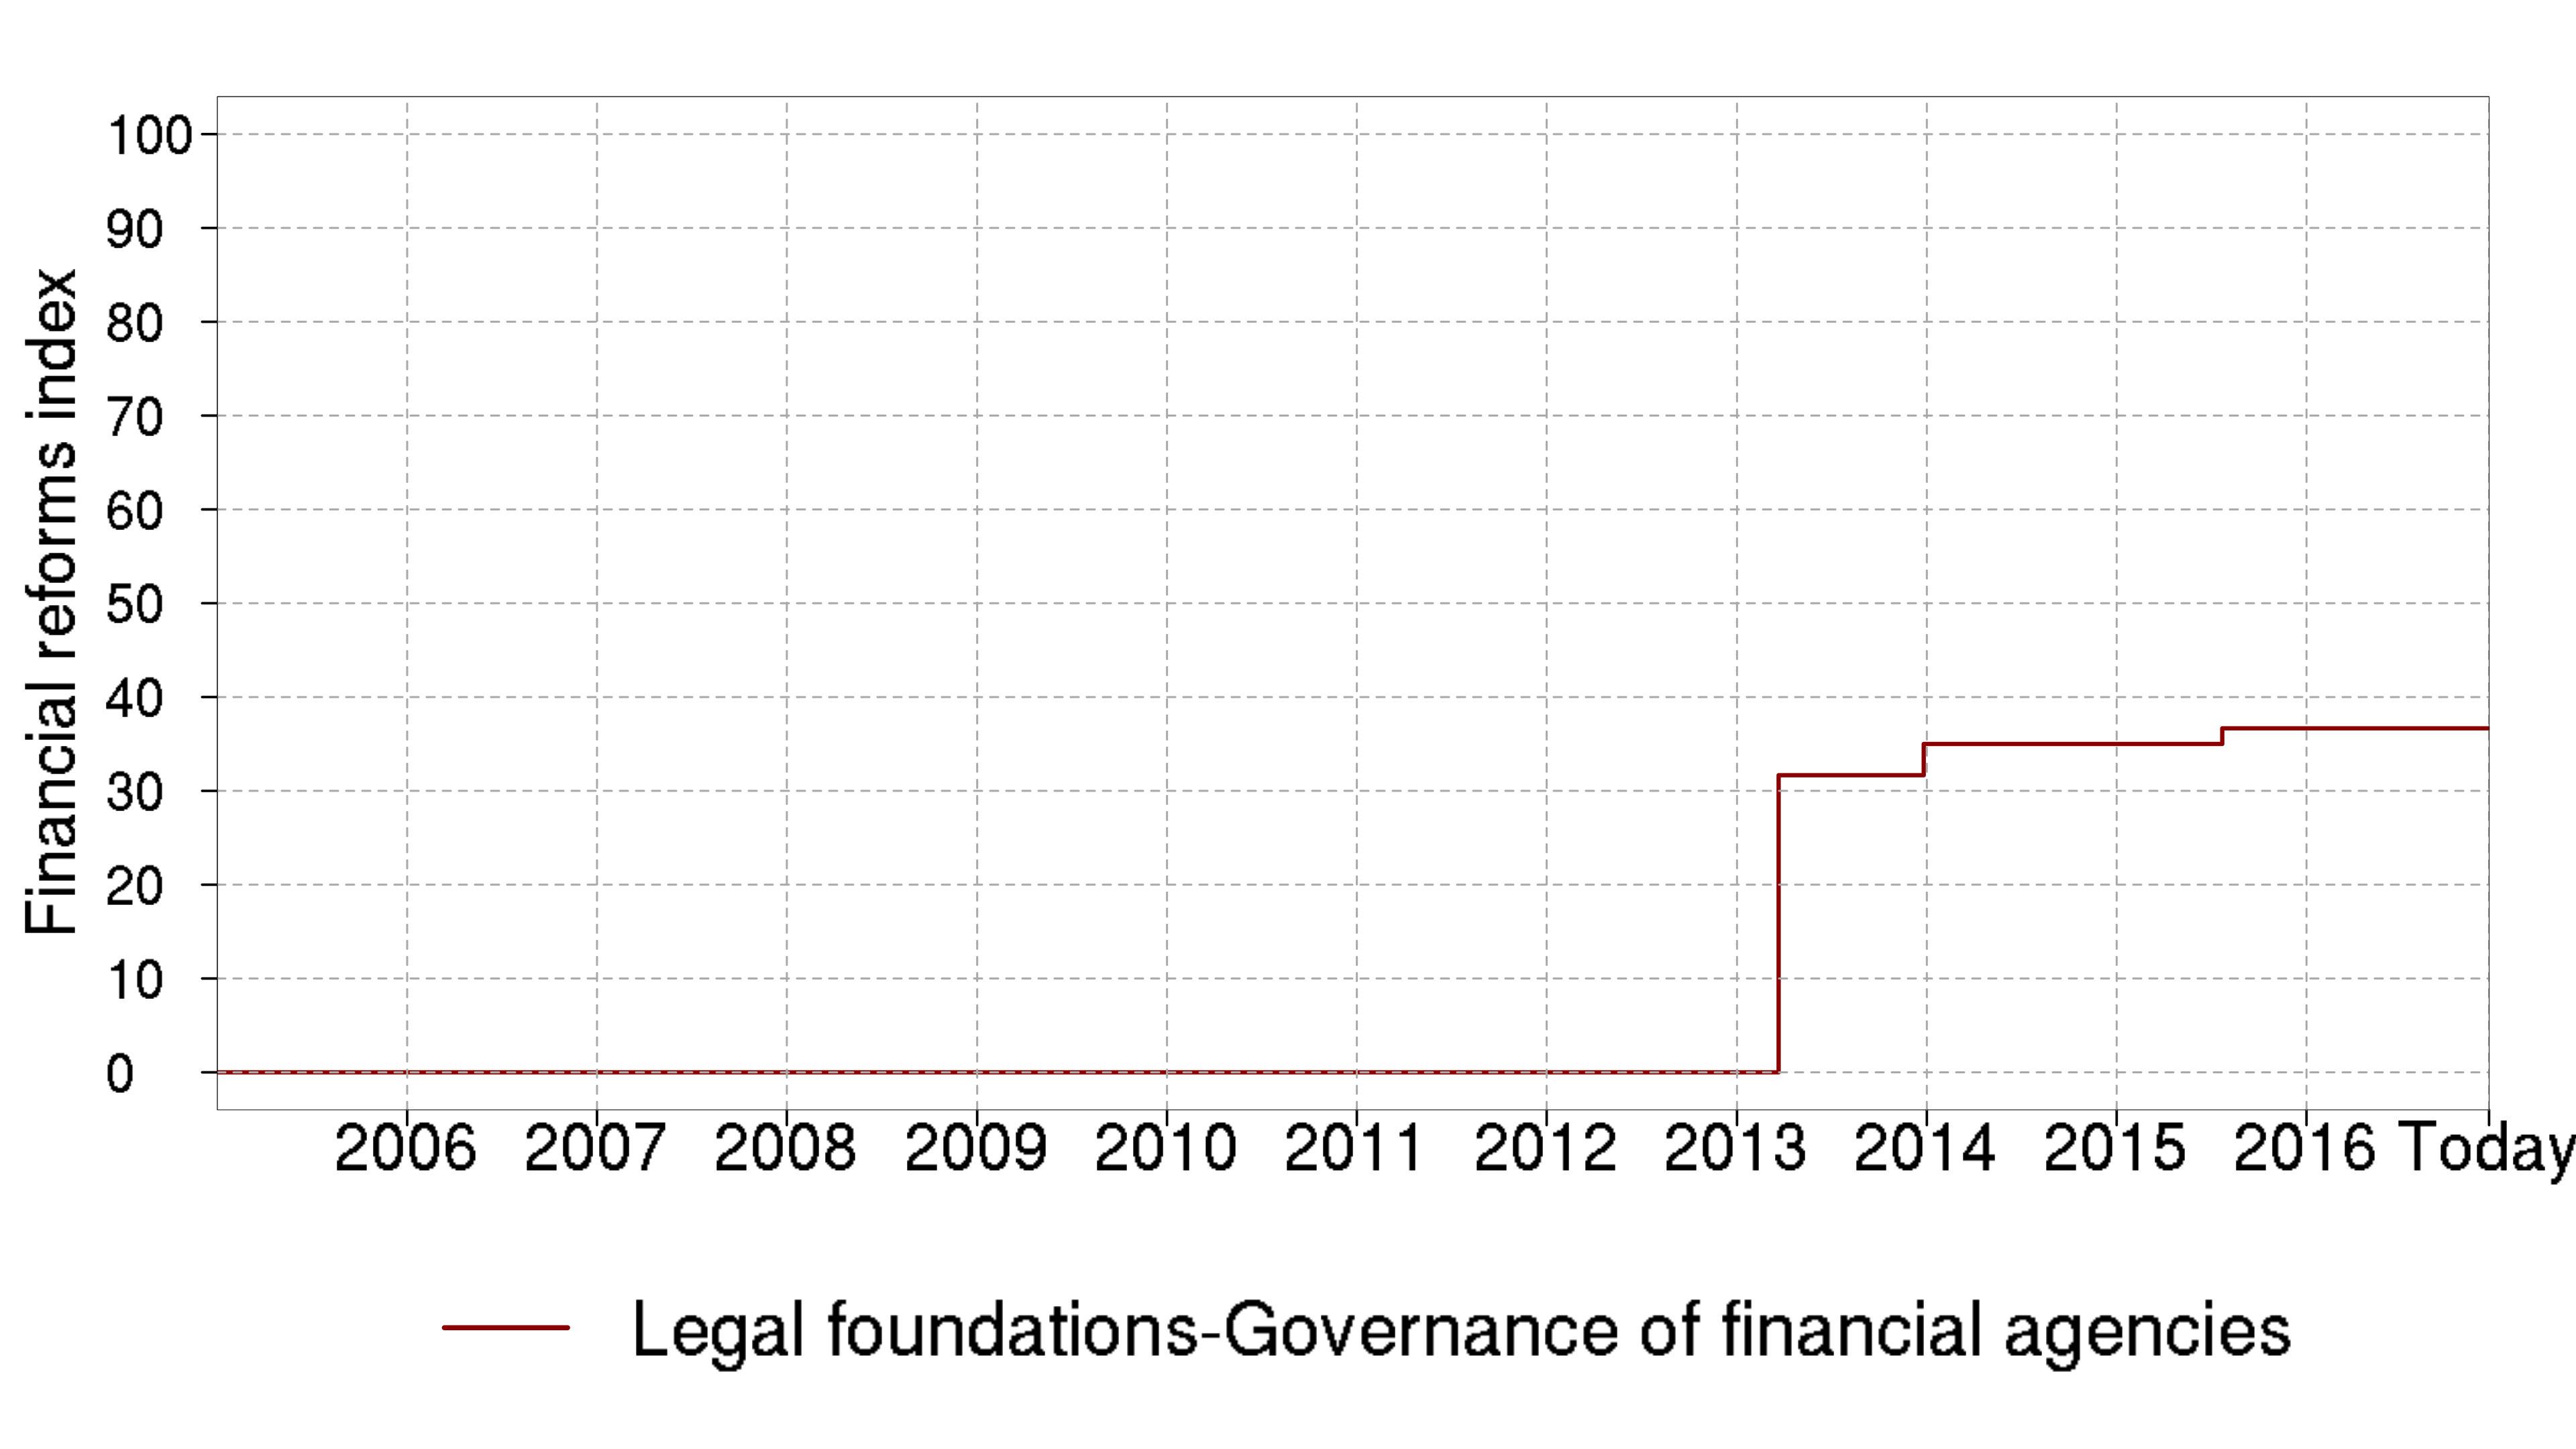
\includegraphics[width=0.65\paperwidth,height=0.45\paperwidth]{../GRAPHS/frm_index_legal_foundations_governance_of_financial_agencies.png}
\end{figure}

\newpage
  \begin{table} [H]
    \caption{Legal foundation: Legislative, executive and quasi judicial functions of financial agencies}
    \begin{threeparttable}
      \begin{footnotesize}
        \resizebox{1\textwidth}{!}{
        
          \glfleaqjfofa{\lfleaqjfofac}{\lfleaqjfofadl}{\lfleaqjfofale}{\lfleaqjfofali}
        }
      \end{footnotesize}
    \end{threeparttable}
  \end{table}
  \begin{figure}[H]
    \caption{Legal foundation: Legislative, executive and quasi judicial functions of financial agencies}
    \centering
    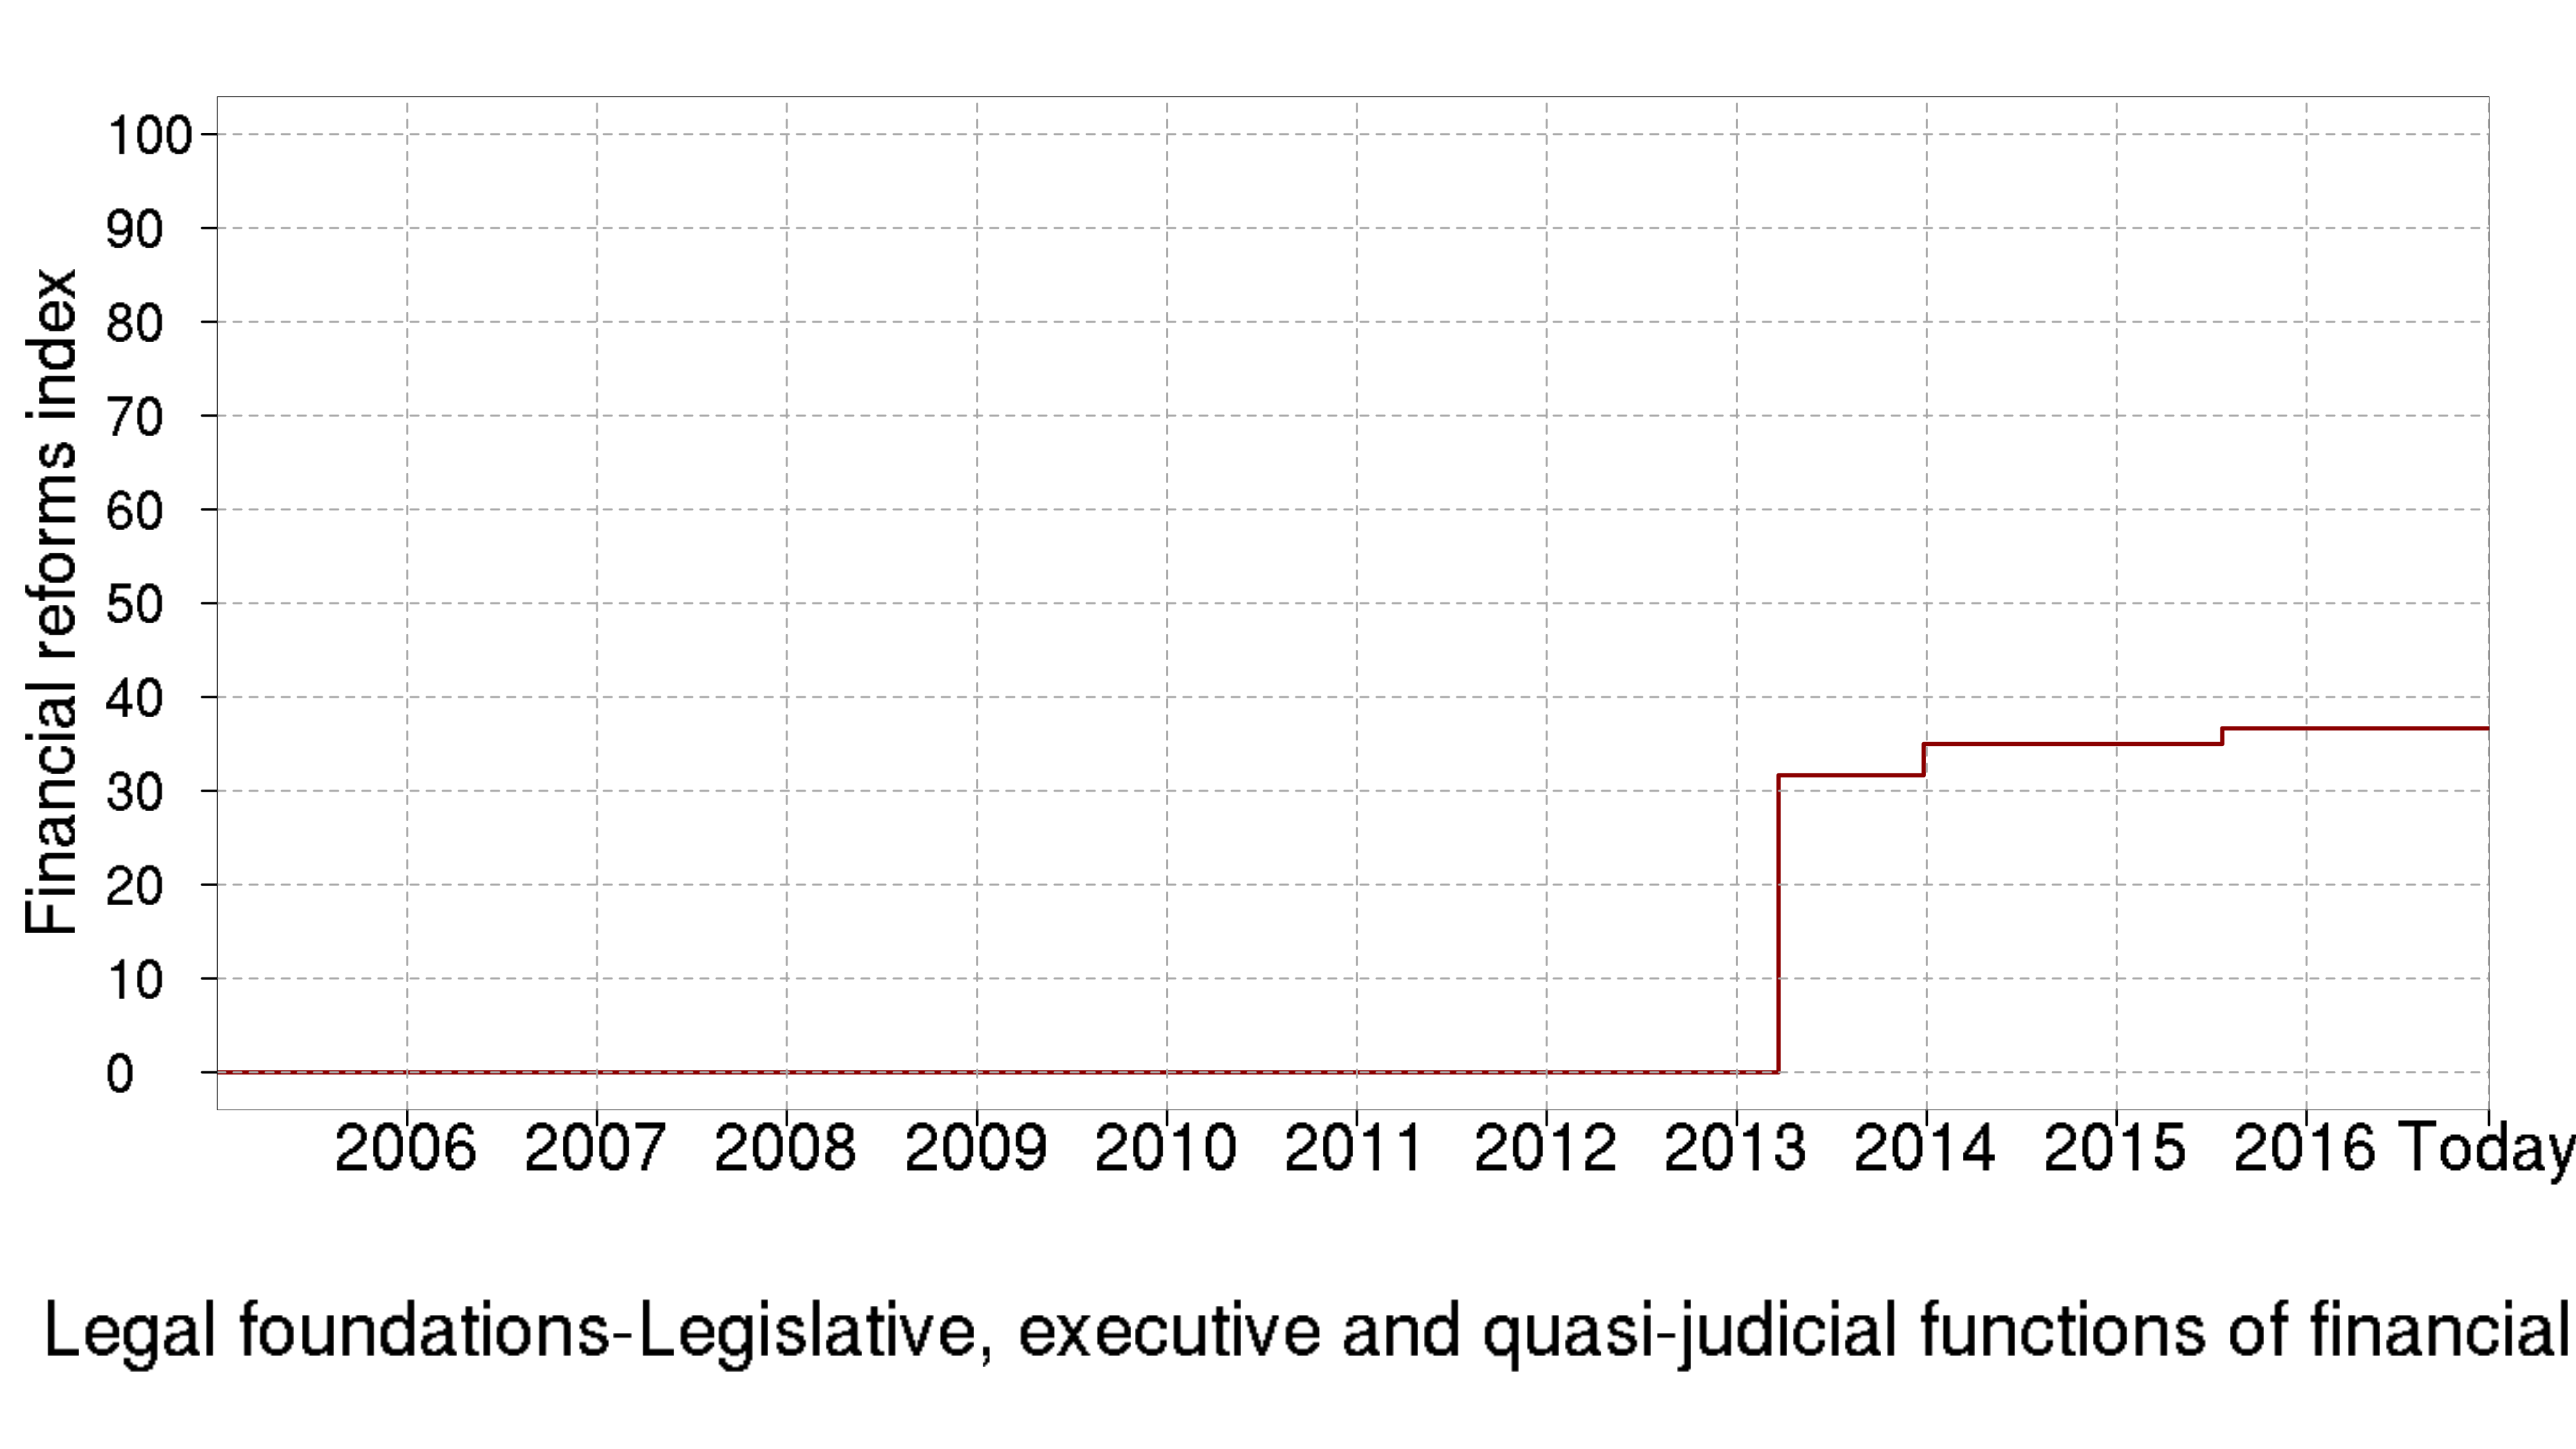
\includegraphics[width=0.65\paperwidth,height=0.45\paperwidth]{../GRAPHS/frm_index_legal_foundations_legislative_executive_and_quasi-judicial_functions_of_financial_agencies.png}
  \end{figure}
  
\newpage
  \begin{table} [H]
    \caption{Legal foundation: Consumer protection}
    \begin{threeparttable}
      \begin{footnotesize}
        \resizebox{1\textwidth}{!}{
          
          \glfcp{\lfcpc}{\lfcpdl}{\lfcple}{\lfcpli}
        }
      \end{footnotesize}
    \end{threeparttable}
  \end{table}
  \begin{figure}[H]
  \centering
    \caption{Legal foundation: Consumer protection}
  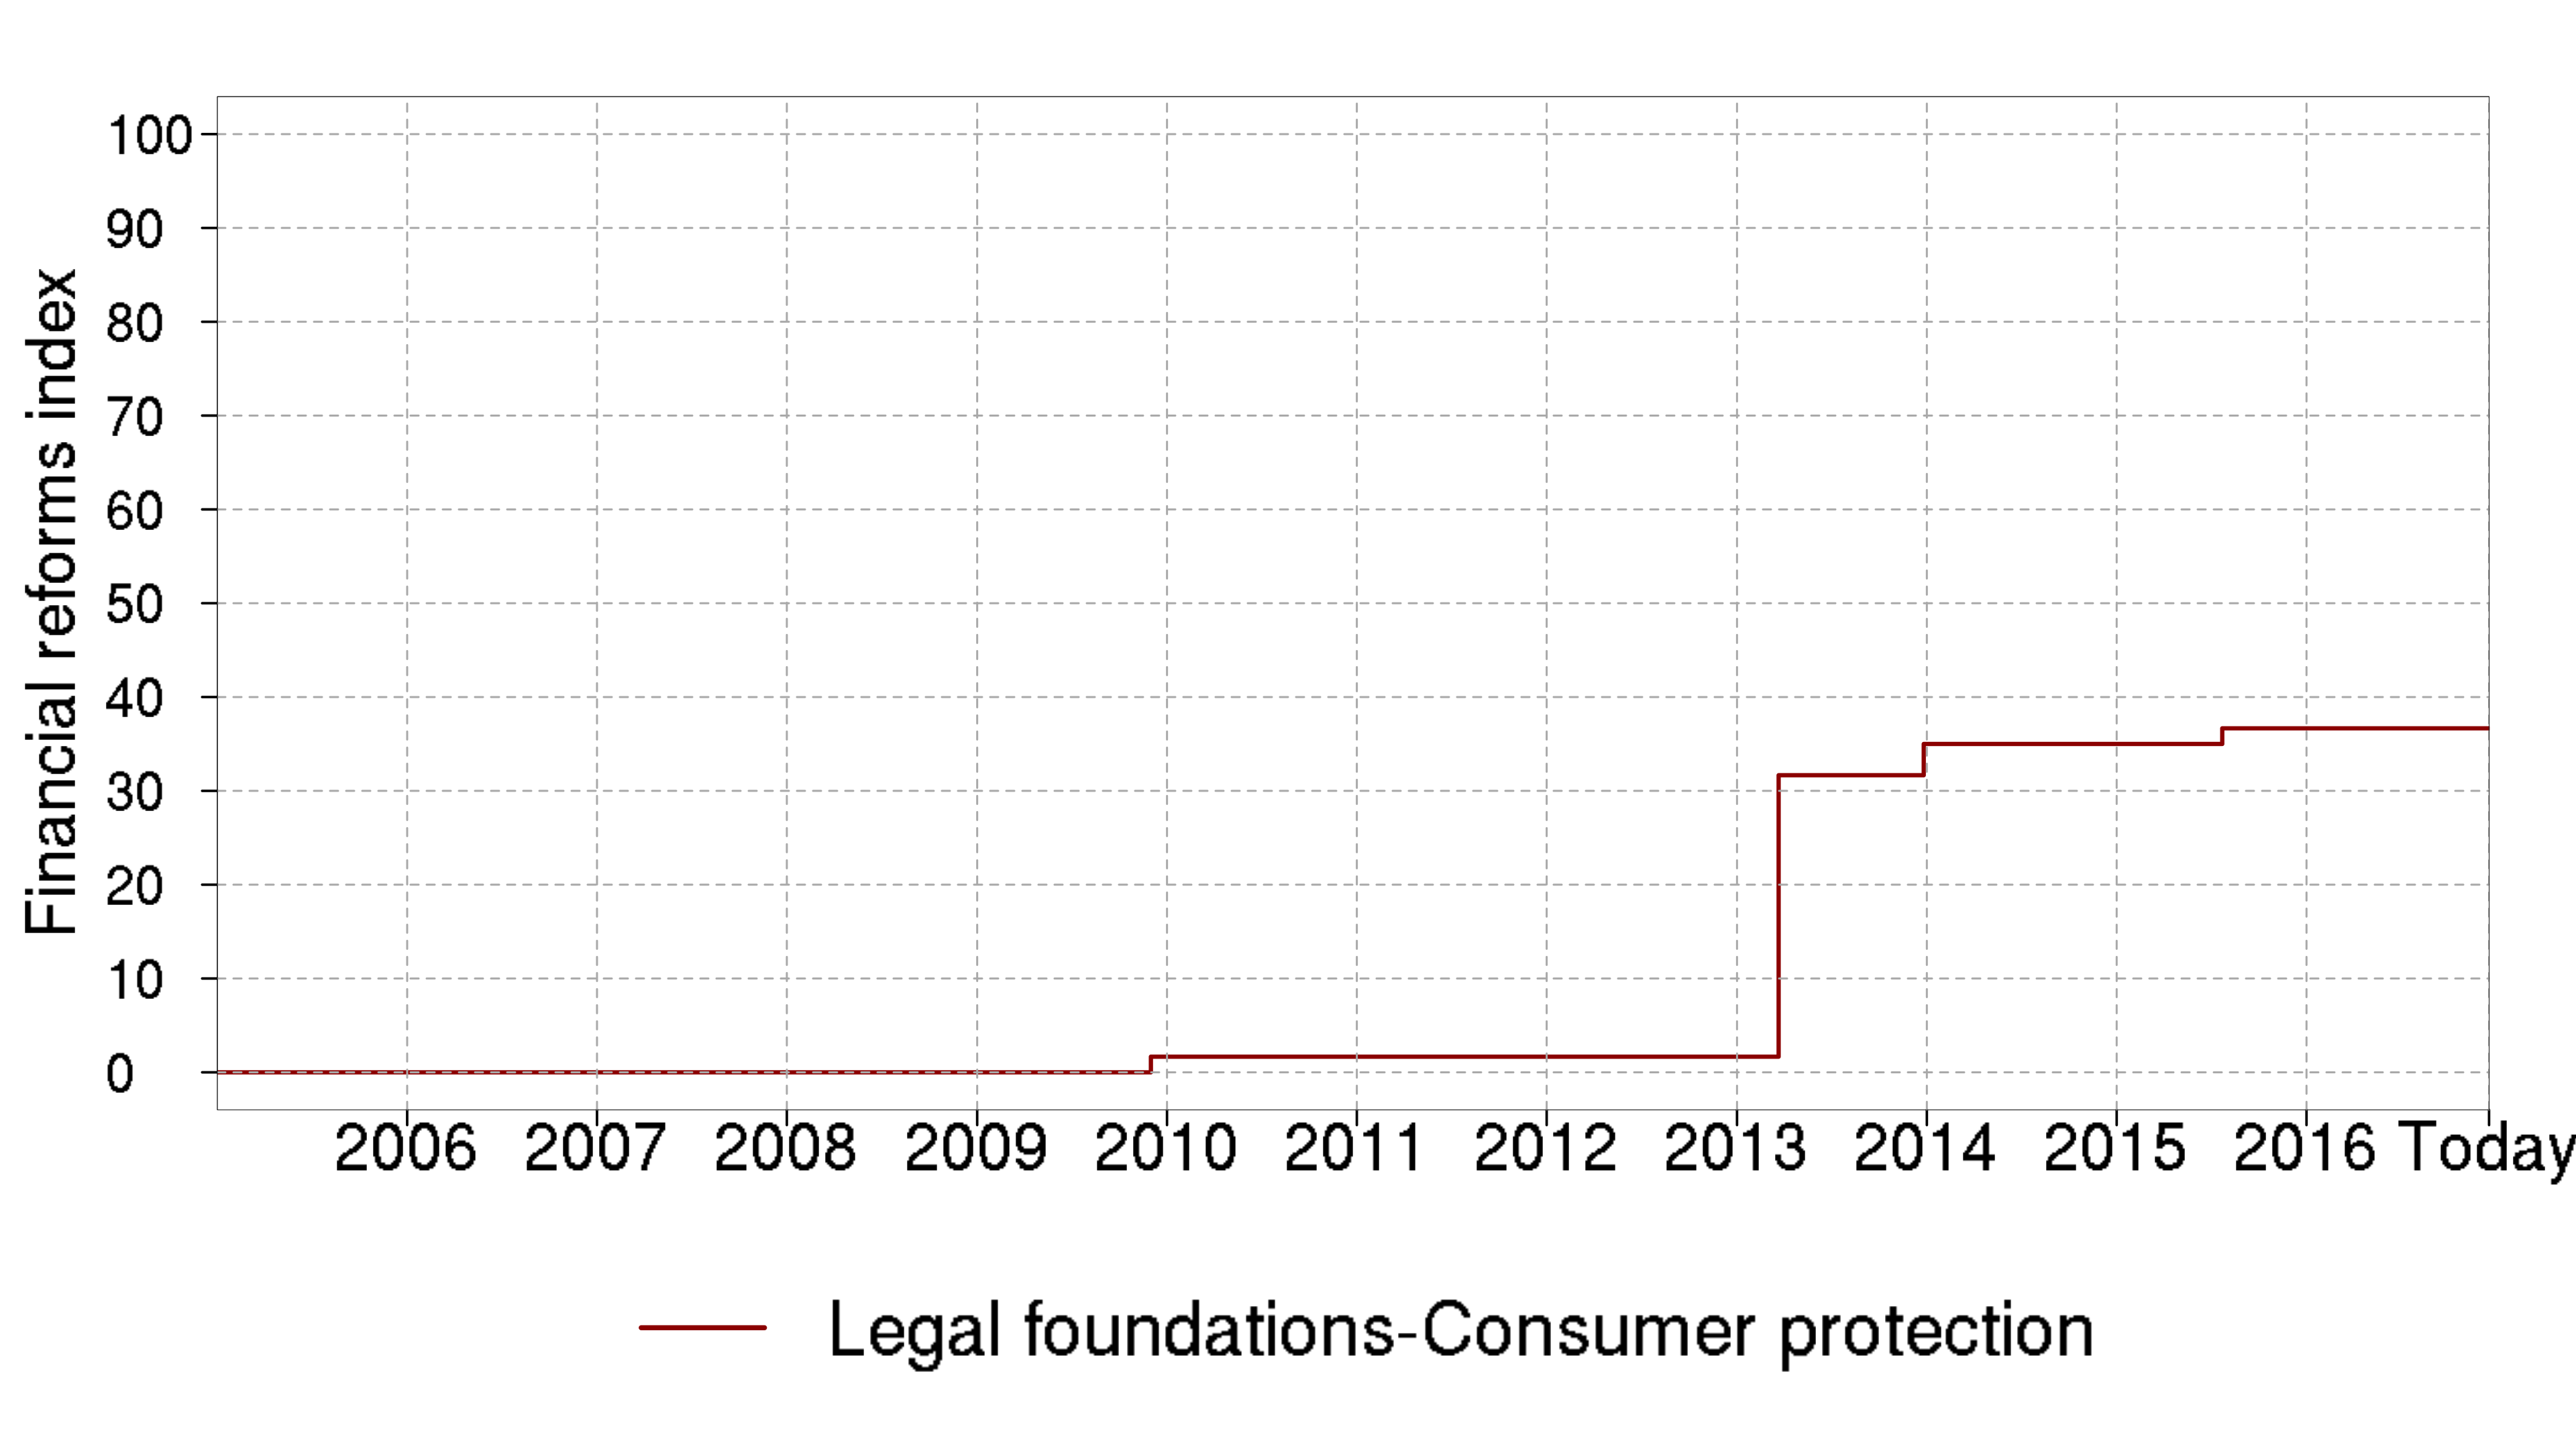
\includegraphics[width=0.65\paperwidth,height=0.45\paperwidth]{../GRAPHS/frm_index_legal_foundations_consumer_protection.png}
  \end{figure}

\newpage
  \begin{table} [H]
    \caption{Legal foundation: Micro-prudential regulations}
    \begin{threeparttable}
      \begin{footnotesize}
        \resizebox{1\textwidth}{!}{
        
          \glfmpr{\lfmprc}{\lfmprdl}{\lfmprle}{\lfmprli}
        }
      \end{footnotesize}
    \end{threeparttable}
  \end{table}
\begin{figure}[H]
  \caption{Legal foundation: Micro-prudential regulations}
 \centering
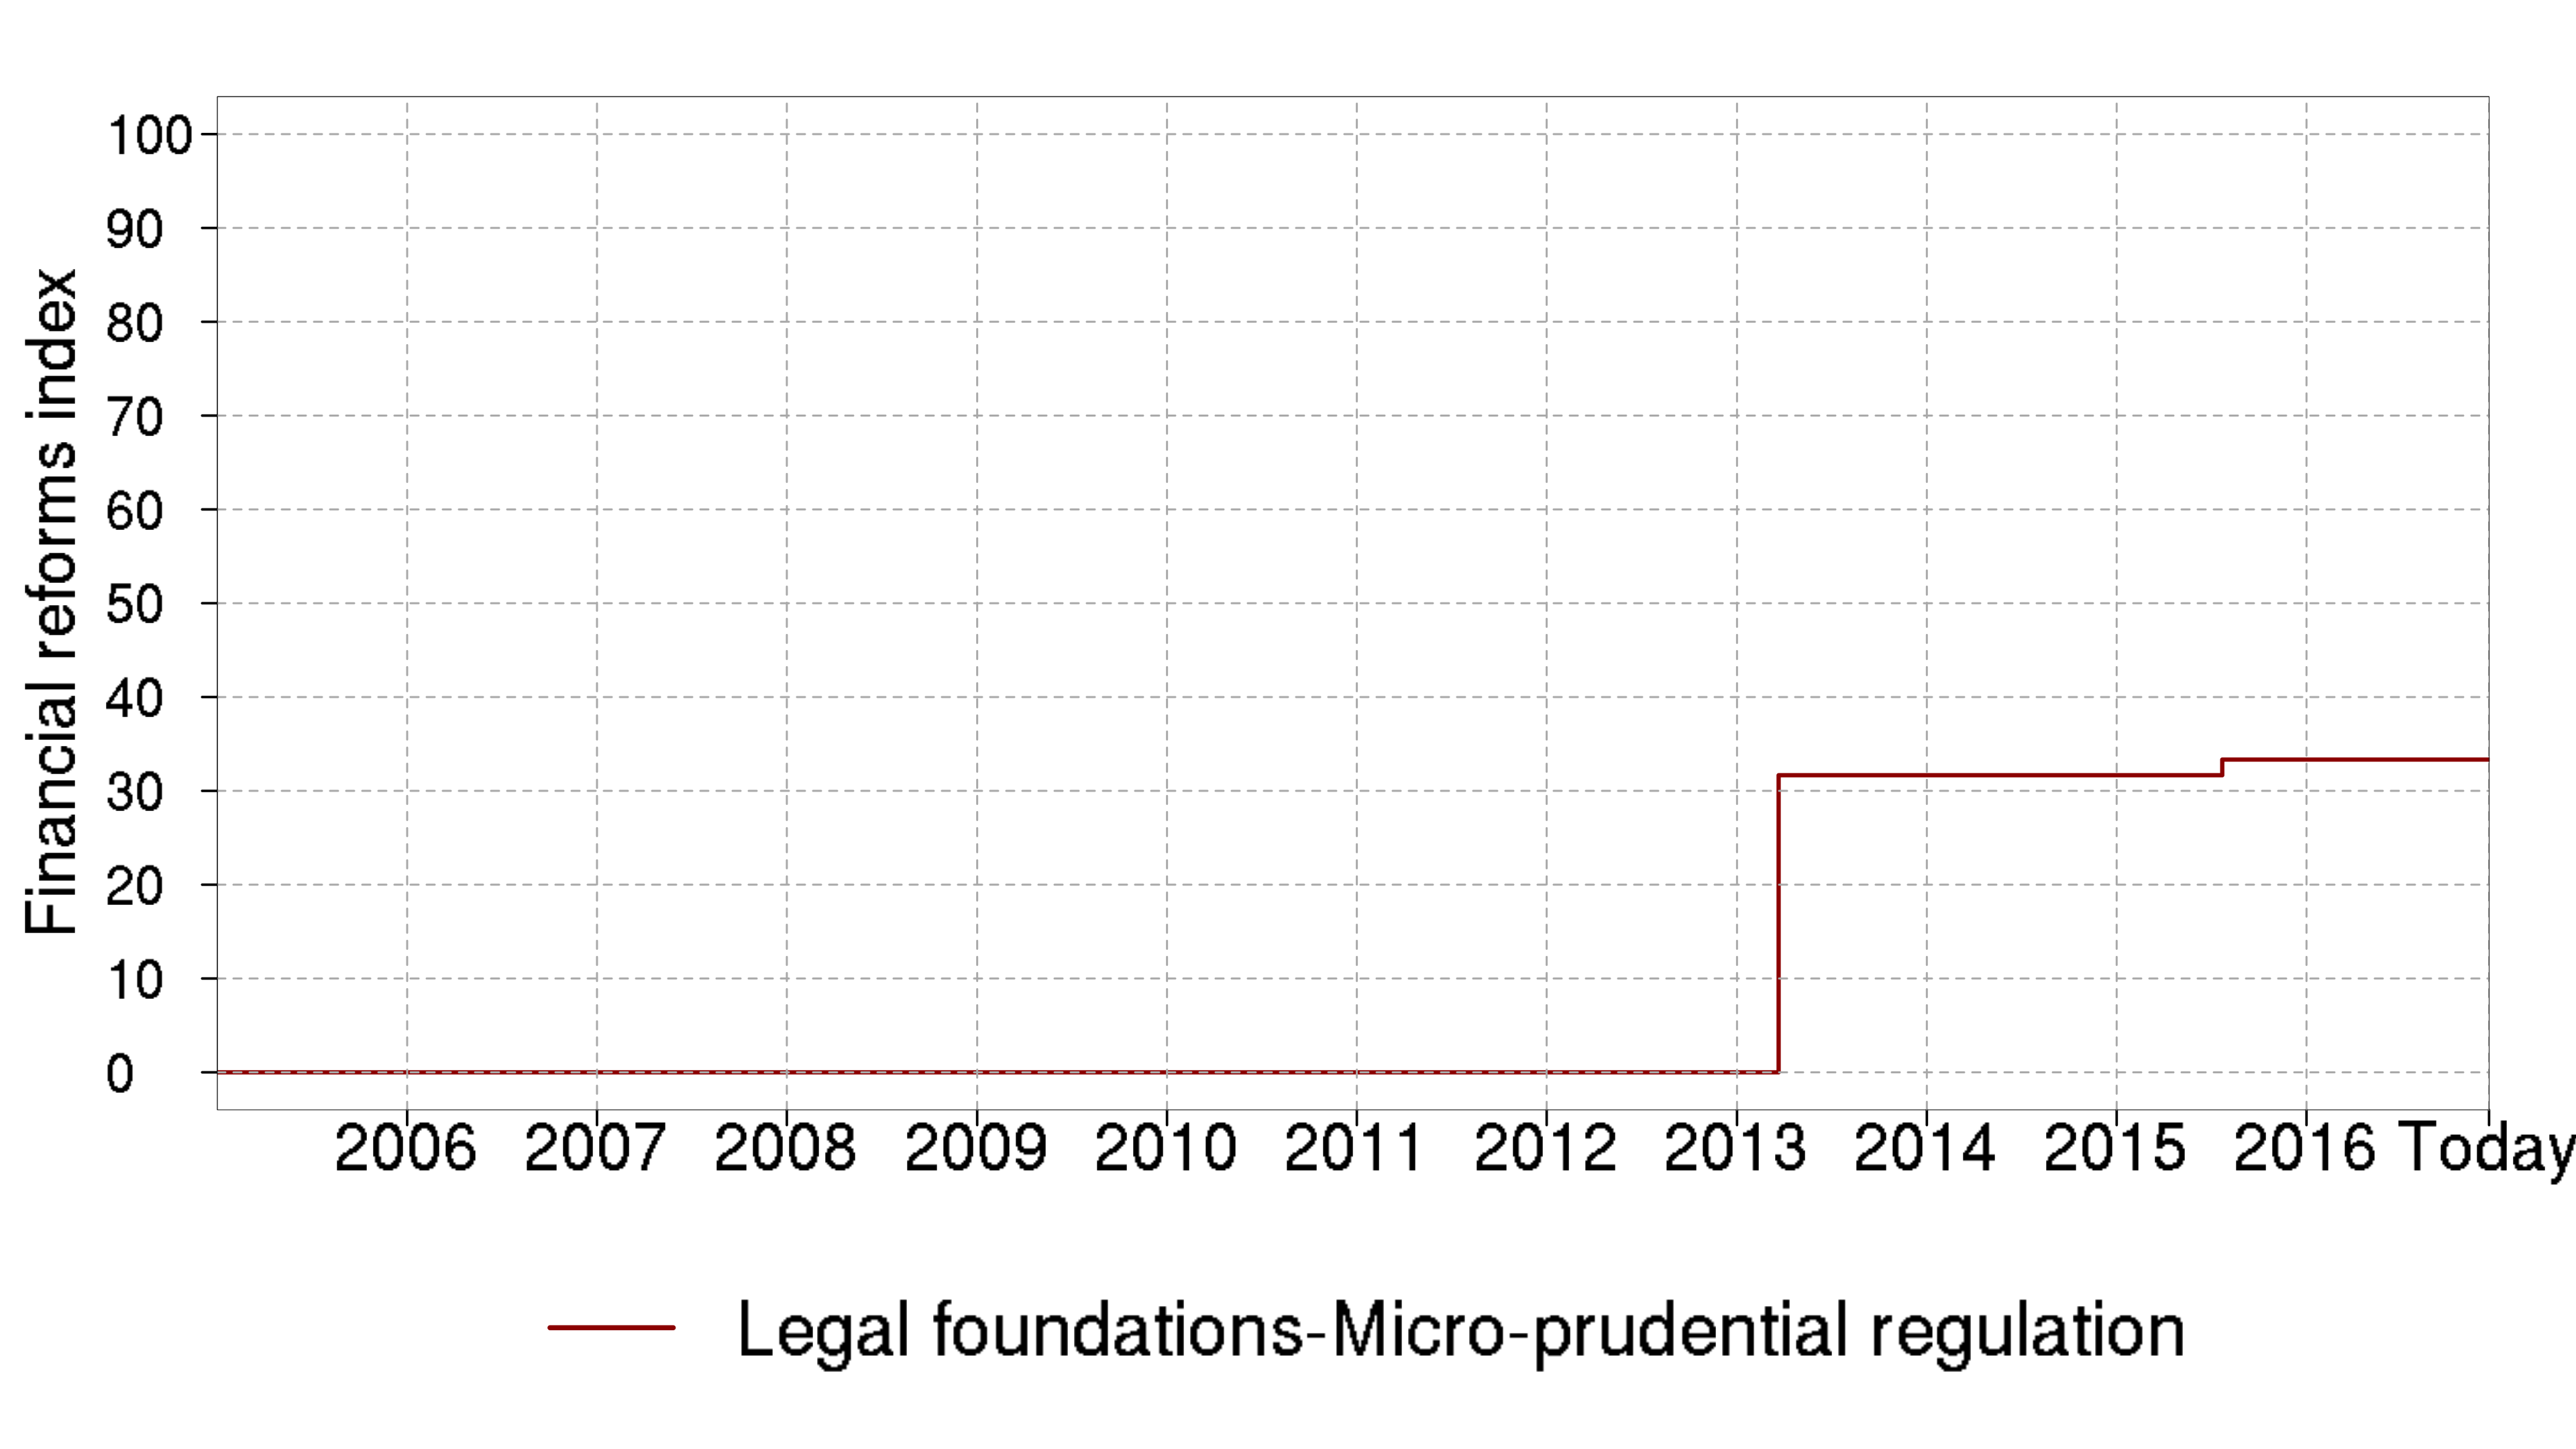
\includegraphics[width=0.65\paperwidth,height=0.45\paperwidth]{../GRAPHS/frm_index_legal_foundations_micro-prudential_regulation.png}
\end{figure}

\newpage
  \begin{table} [H]
    \caption{Legal foundation: Development}
    \begin{threeparttable}
      \begin{footnotesize}
        \resizebox{1\textwidth}{!}{
        
          \glfd{\lfdc}{\lfddl}{\lfdle}{\lfdli}
        }
      \end{footnotesize}
    \end{threeparttable}
  \end{table}
\begin{figure}[H]
   \caption{Legal foundation: Development}
 \centering
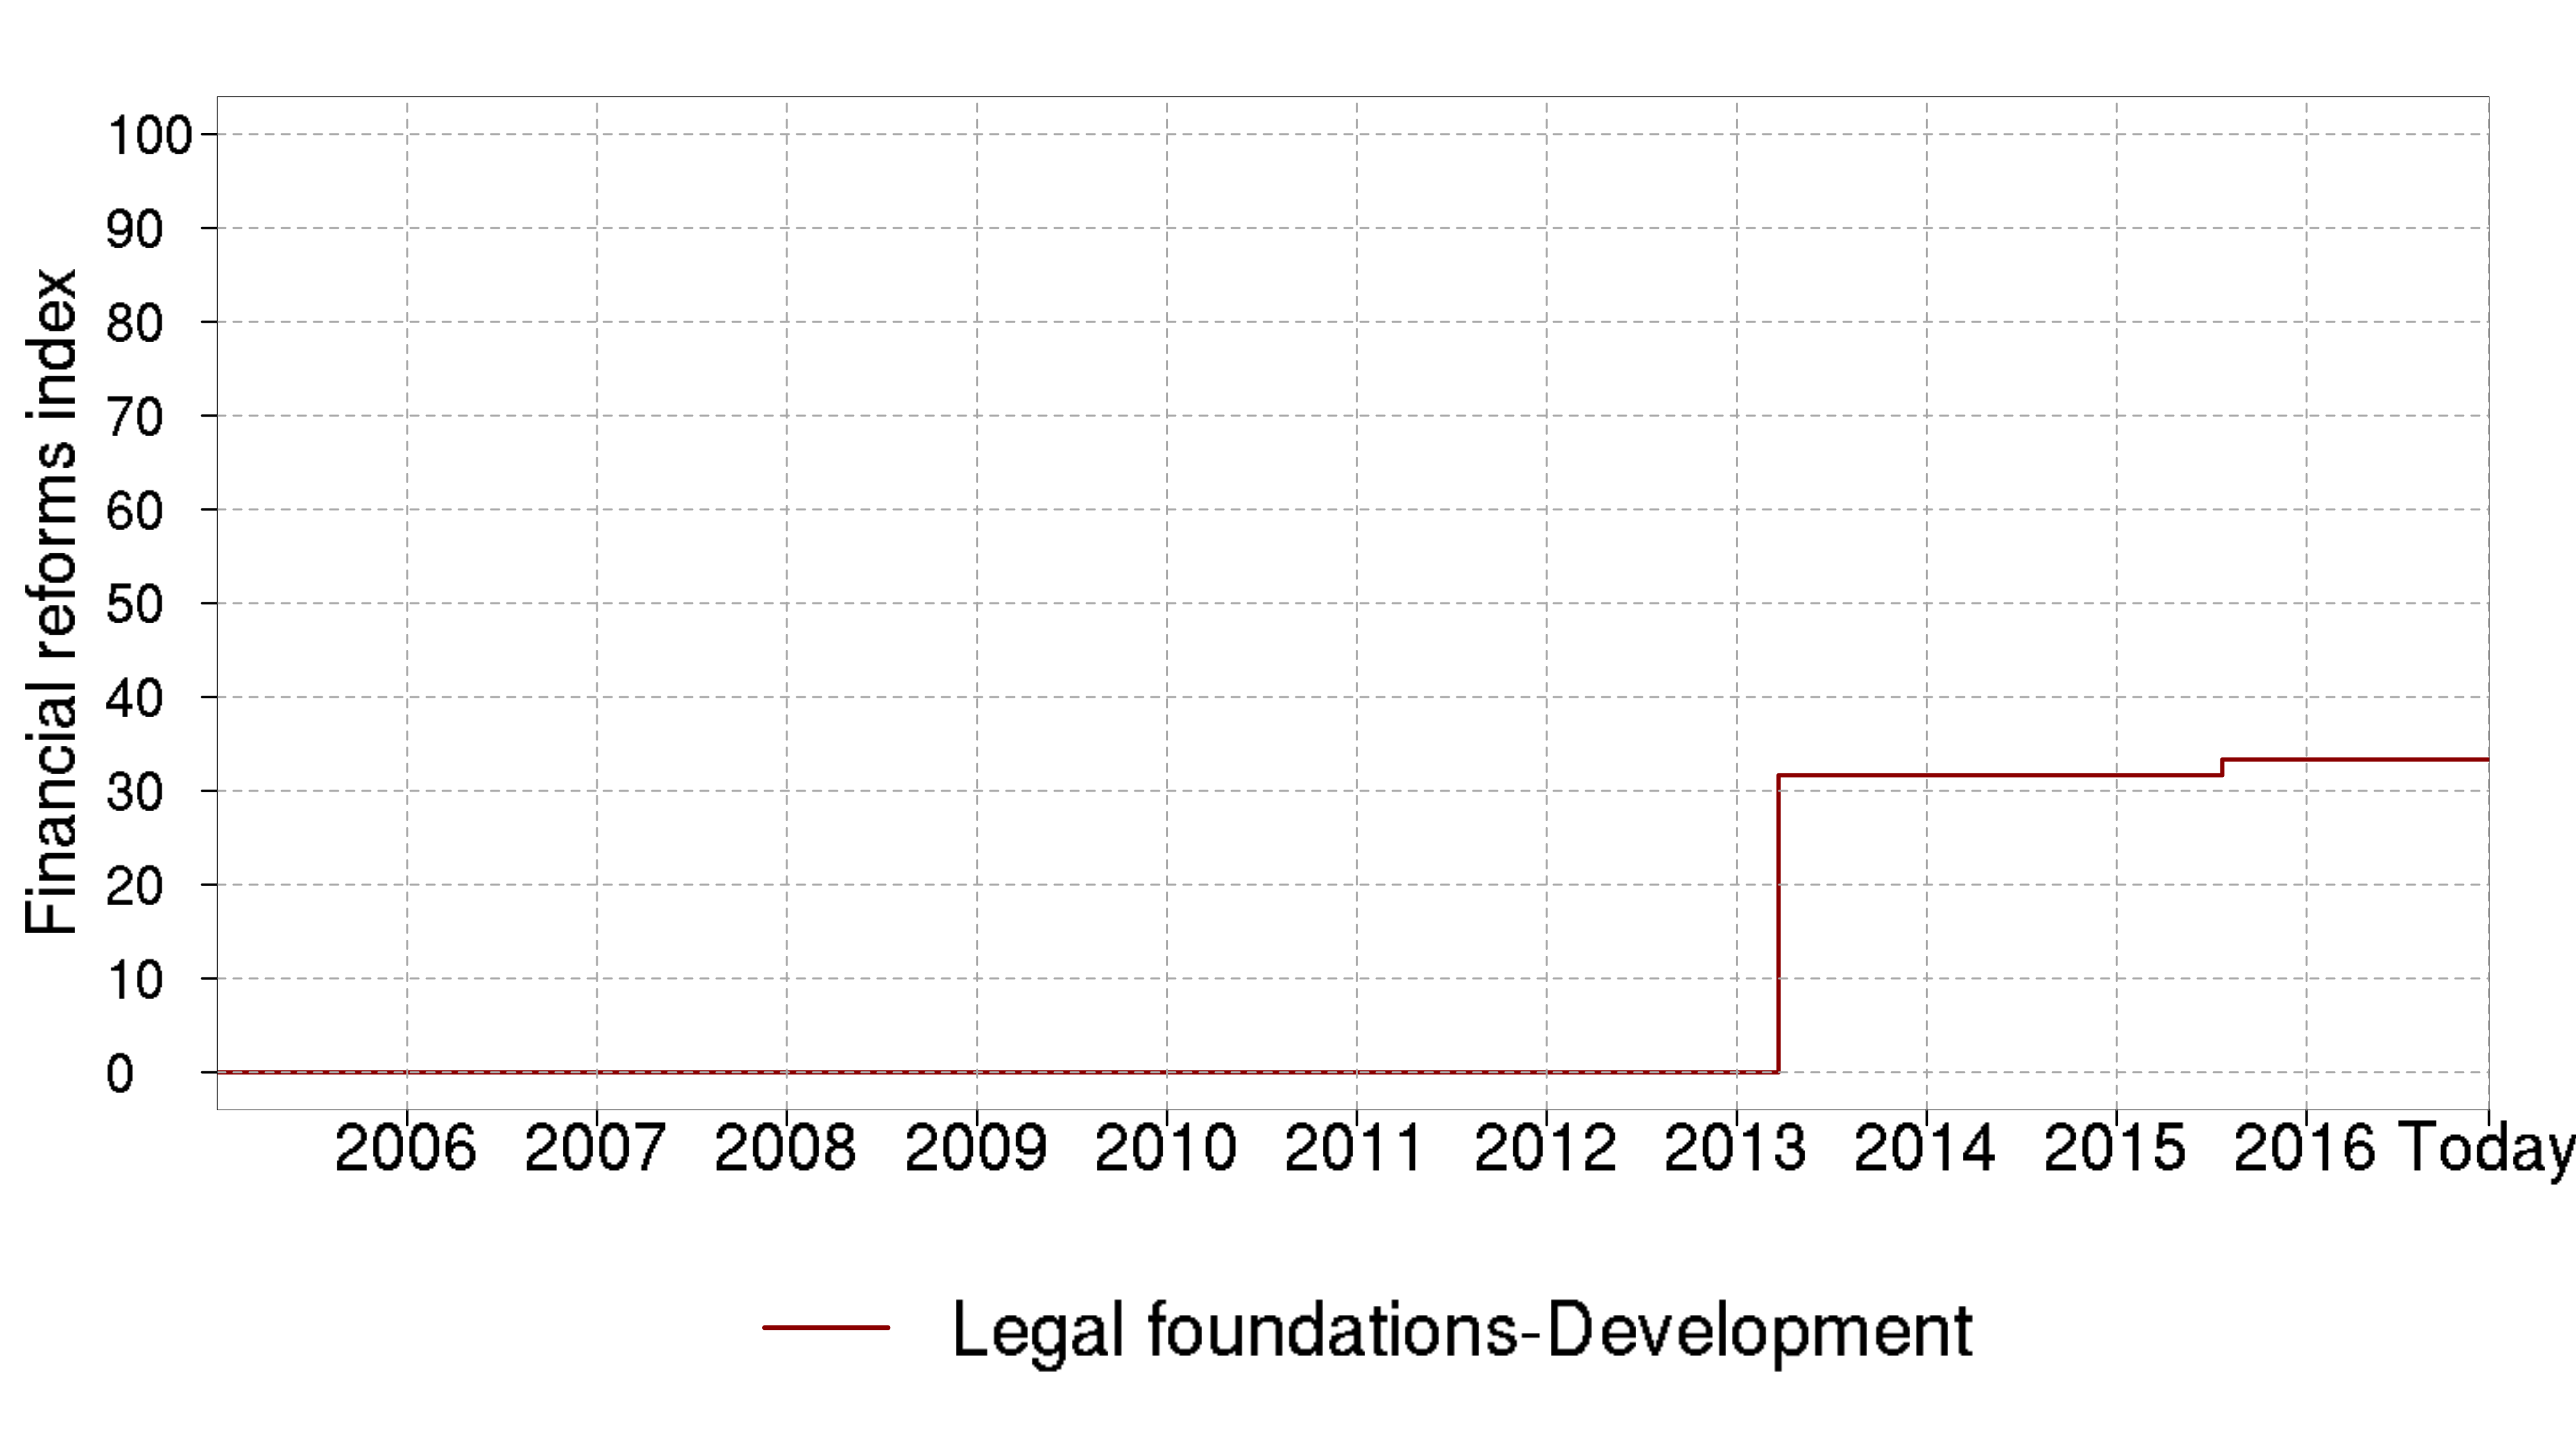
\includegraphics[width=0.65\paperwidth,height=0.45\paperwidth]{../GRAPHS/frm_index_legal_foundations_development.png}
\end{figure}

\newpage
  \begin{table} [H]
    \caption{Legal foundation: Capital controls}
    \begin{threeparttable}
      \begin{footnotesize}
        \resizebox{1\textwidth}{!}{
        
          \glfcc{\lfccc}{\lfccdl}{\lfccle}{\lfccli}
        }
      \end{footnotesize}
    \end{threeparttable}
  \end{table}
\begin{figure}[H]
   \caption{Legal foundation: Capital controls}
 \centering
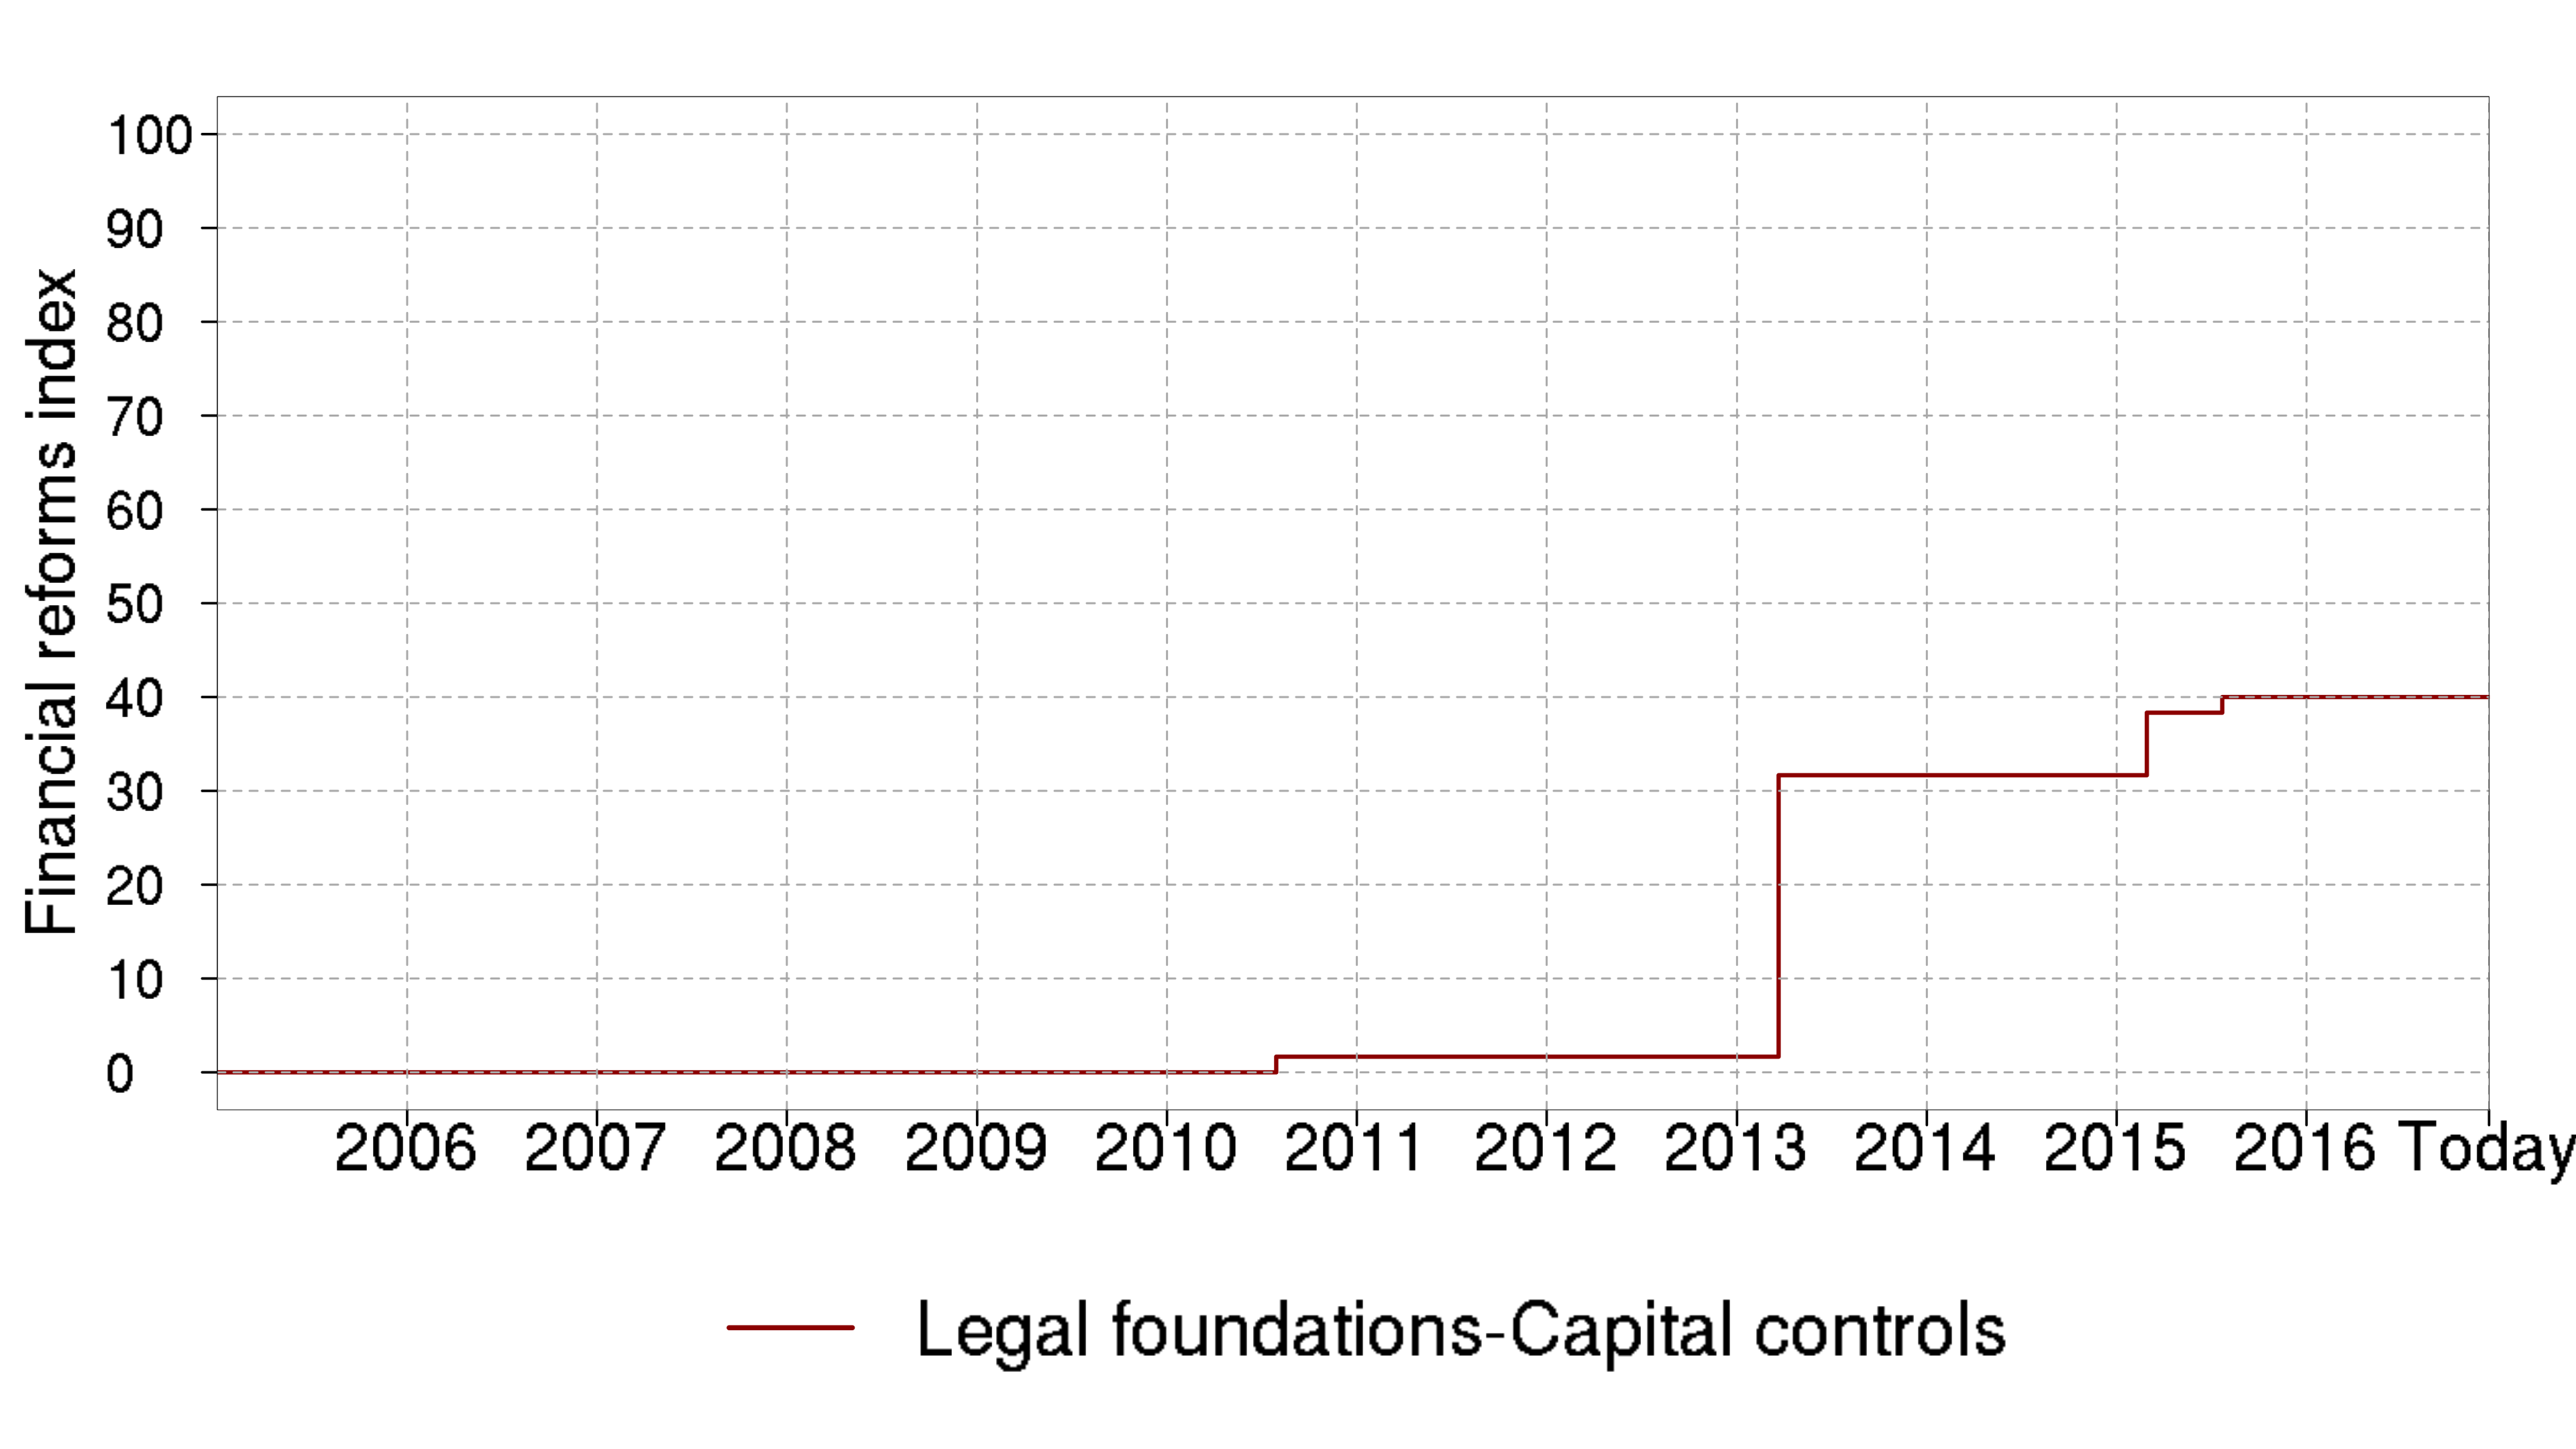
\includegraphics[width=0.65\paperwidth,height=0.45\paperwidth]{../GRAPHS/frm_index_legal_foundations_capital_controls.png}
\end{figure}

\newpage
  \begin{table} [H]
    \caption{Legal foundation: Resolution}
    \begin{threeparttable}
      \begin{footnotesize}
        \resizebox{1\textwidth}{!}{
        
          \glfr{\lfrc}{\lfrdl}{\lfrle}{\lfrli}
        }
      \end{footnotesize}
    \end{threeparttable}
  \end{table}
\begin{figure}[H]
   \caption{Legal foundation: Resolution}
 \centering
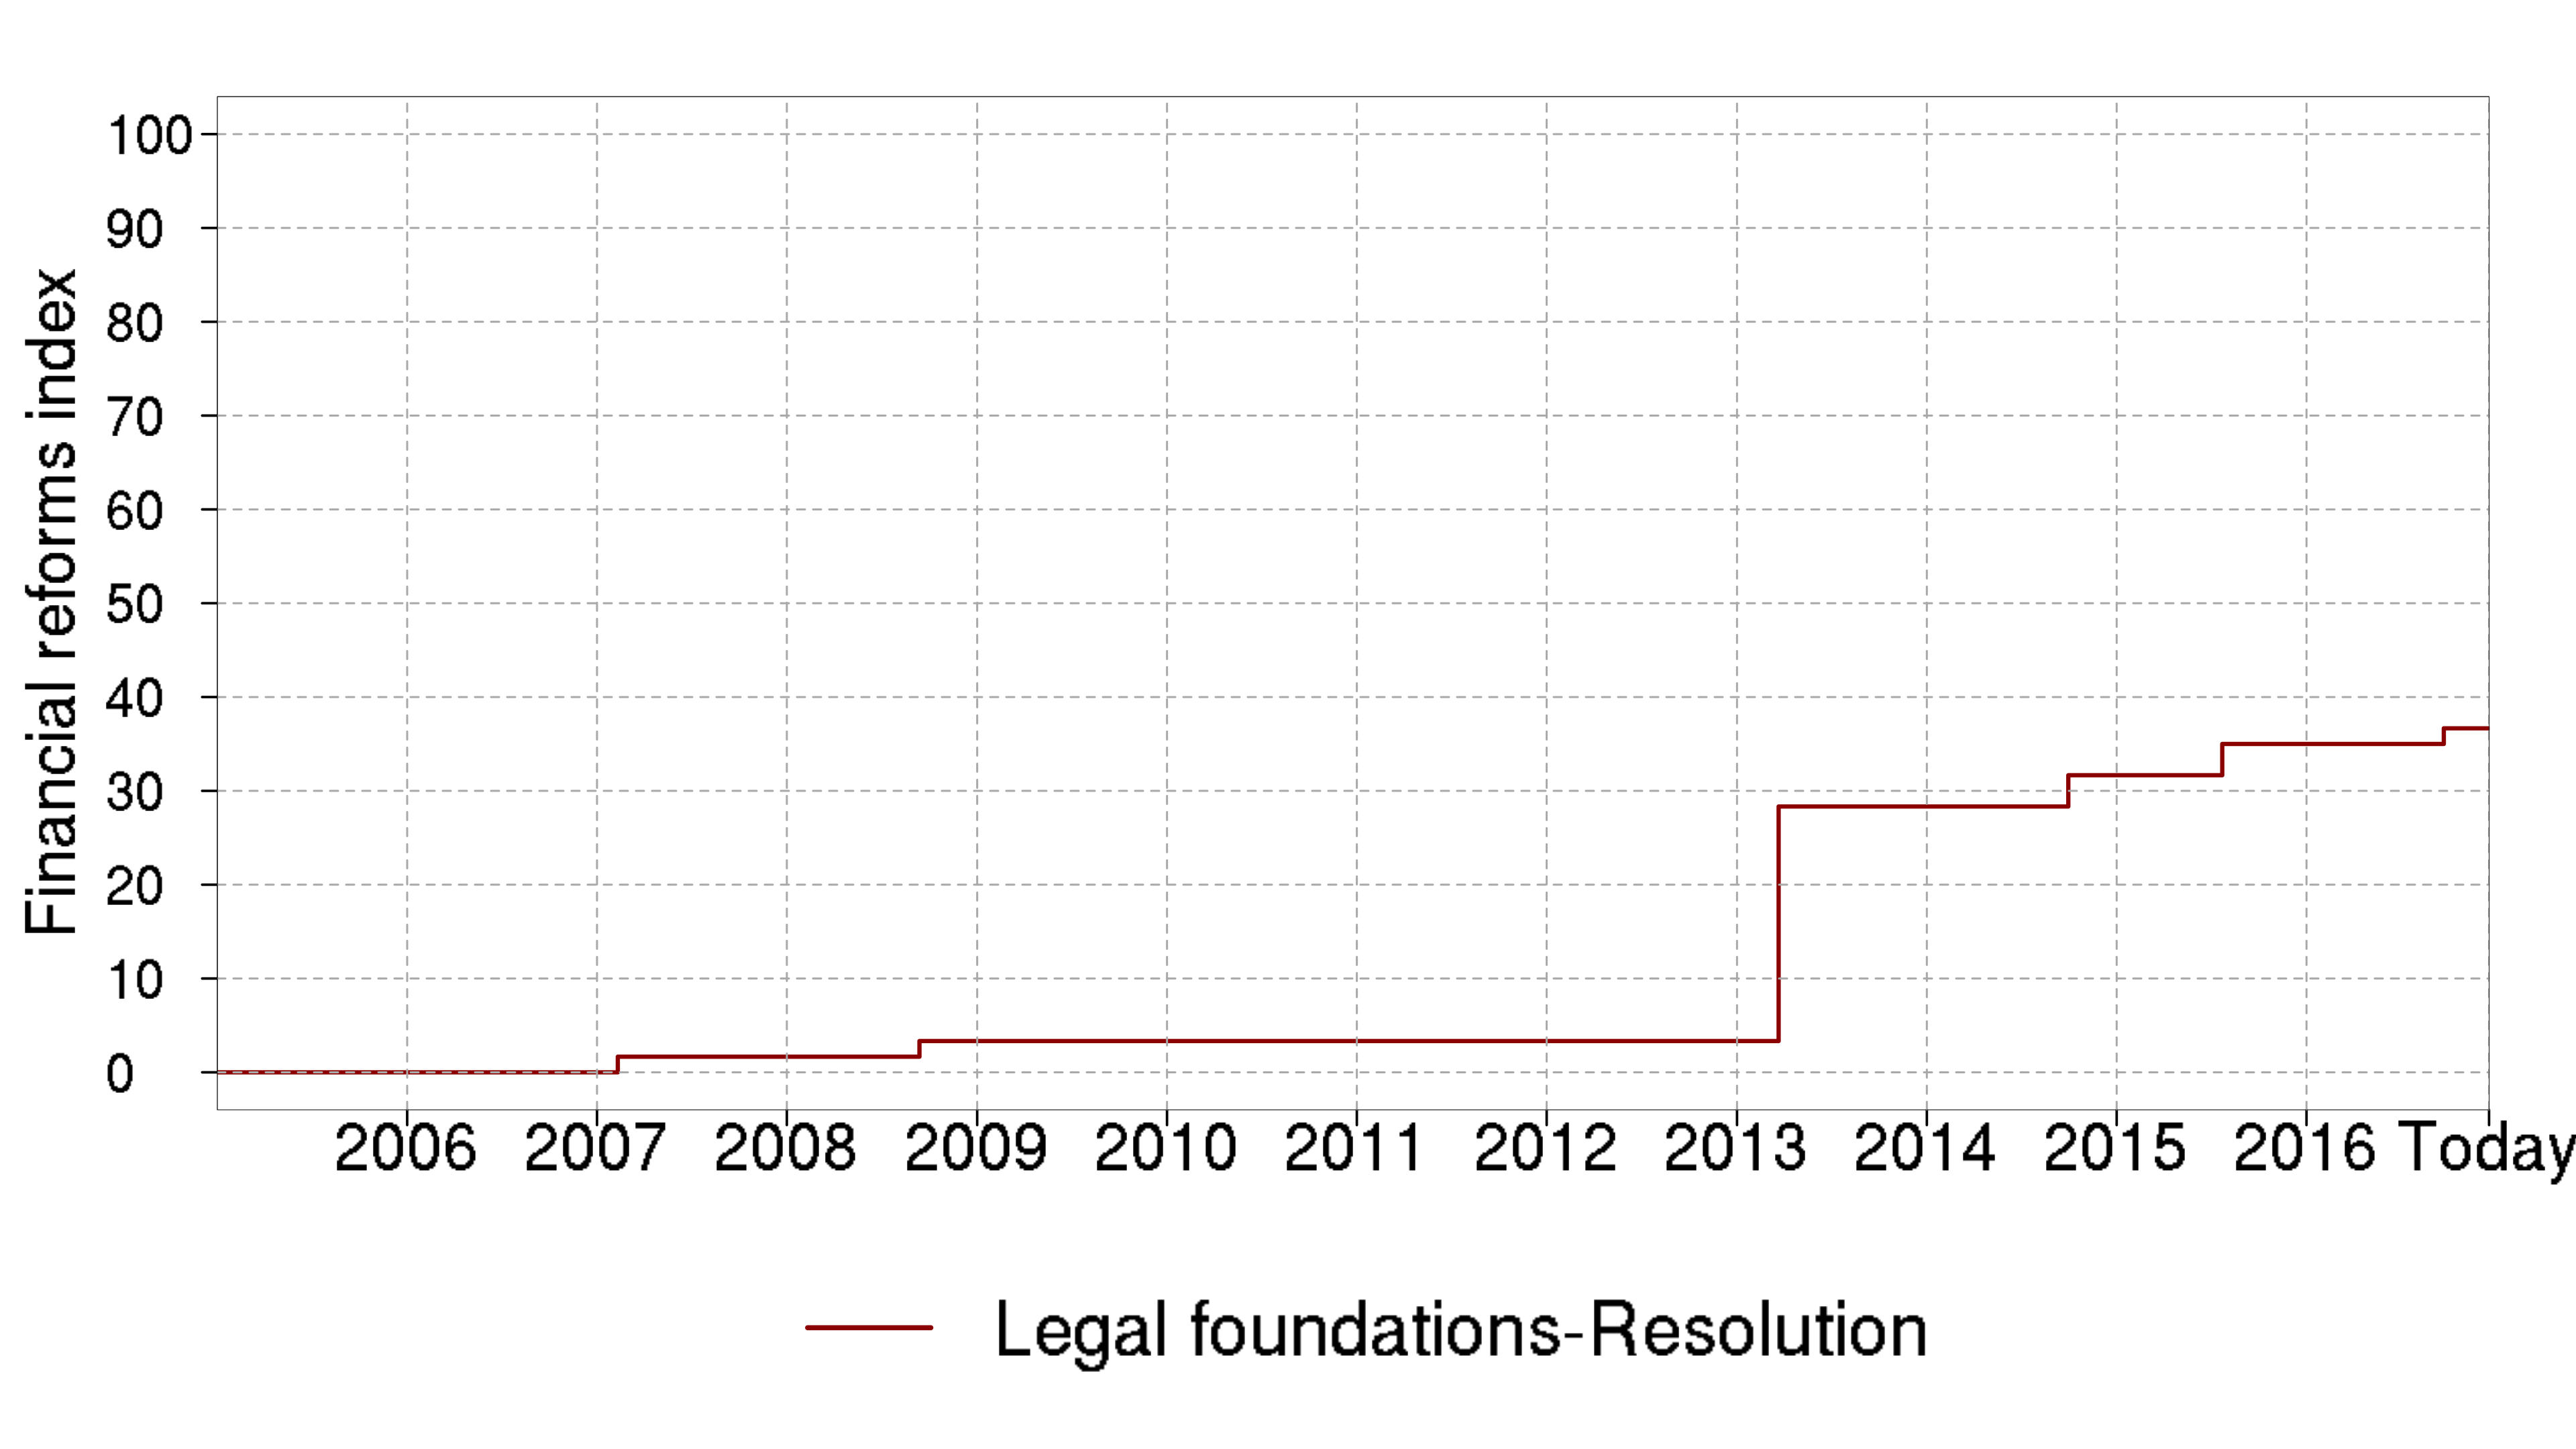
\includegraphics[width=0.65\paperwidth,height=0.45\paperwidth]{../GRAPHS/frm_index_legal_foundations_resolution.png}
\end{figure}

\newpage
  \begin{table} [H]
    \caption{Legal foundation: Financial redress agency}
    \begin{threeparttable}
      \begin{footnotesize}
        \resizebox{1\textwidth}{!}{
        
          \glffra{\lffrac}{\lffradl}{\lffrale}{\lffrali}
        }
      \end{footnotesize}
    \end{threeparttable}
  \end{table}
\begin{figure}[H]
  \caption{Legal foundation: Financial redress agency}
\centering
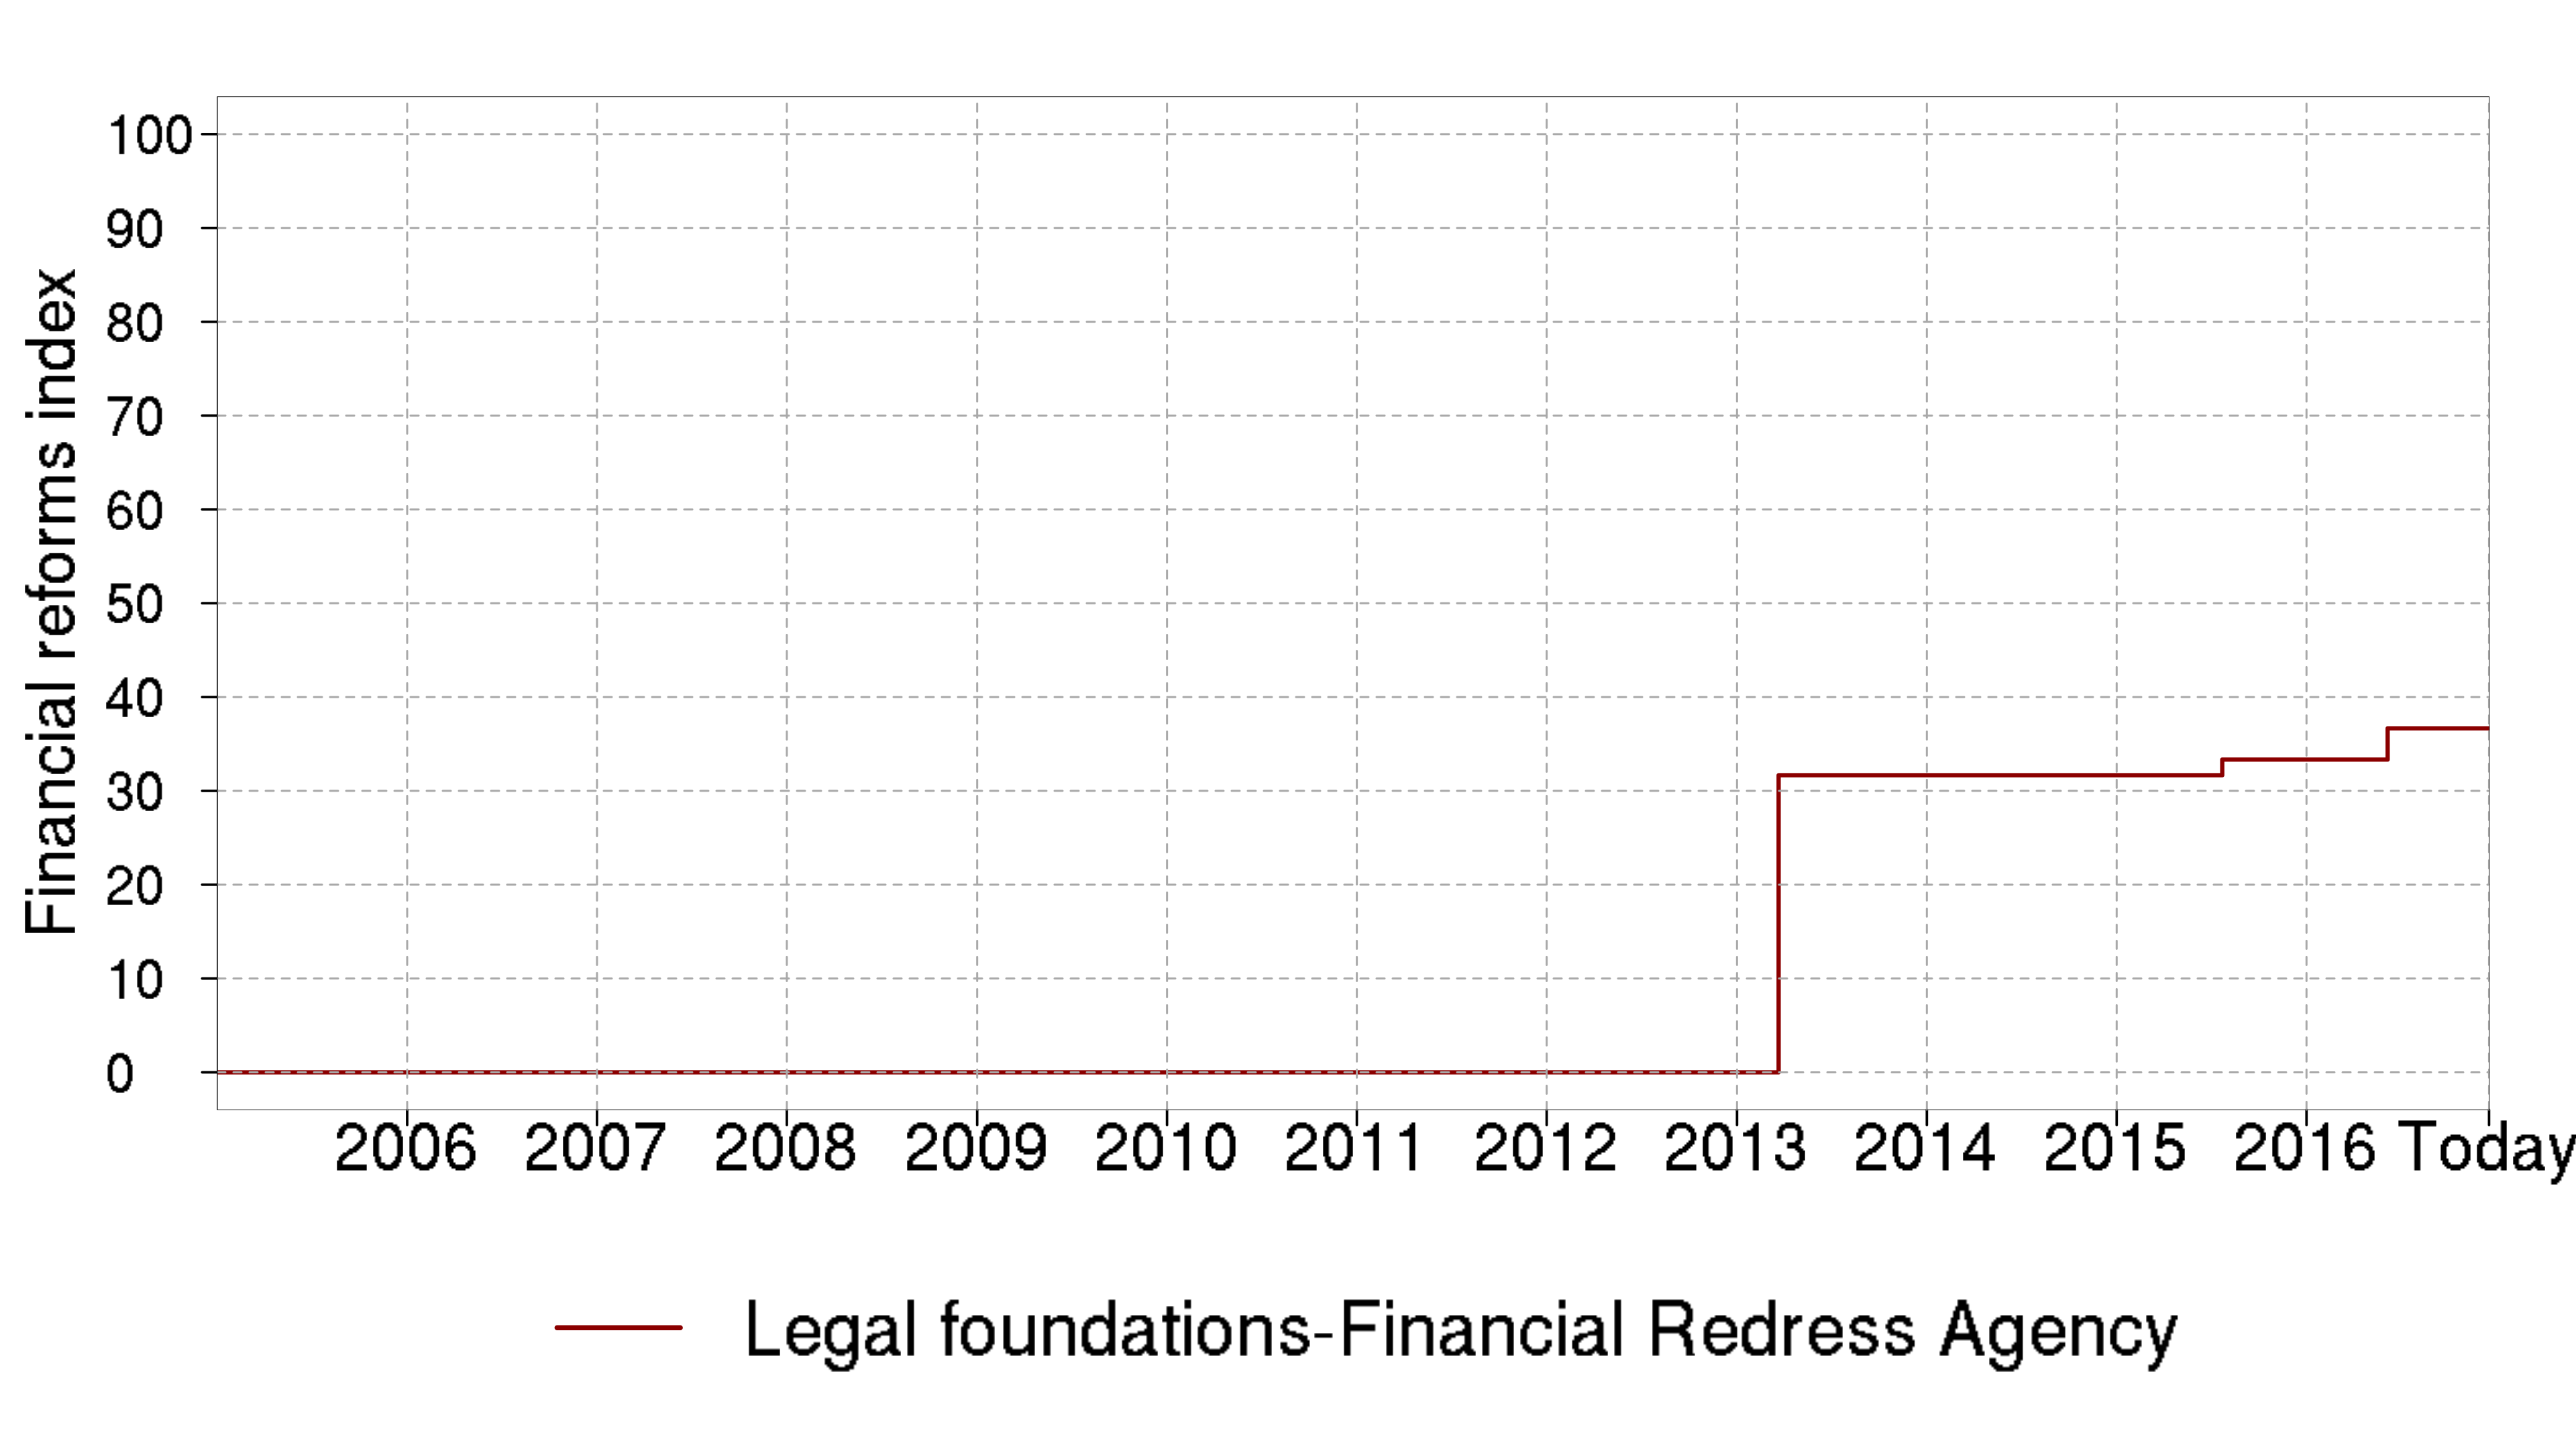
\includegraphics[width=0.65\paperwidth,height=0.45\paperwidth]{../GRAPHS/frm_index_legal_foundations_financial_redress_agency.png}
\end{figure}
  
\newpage
  \begin{table} [H]
    \caption{Legal foundation: Reserve Bank of India}
    \begin{threeparttable}
      \begin{footnotesize}
        \resizebox{1\textwidth}{!}{
        
          \glfrbi{\lfrbic}{\lfrbidl}{\lfrbile}{\lfrbili}
        }
      \end{footnotesize}
    \end{threeparttable}
  \end{table}
\begin{figure}[H]
  \caption{Legal foundation: Reserve Bank of India}
  
\centering
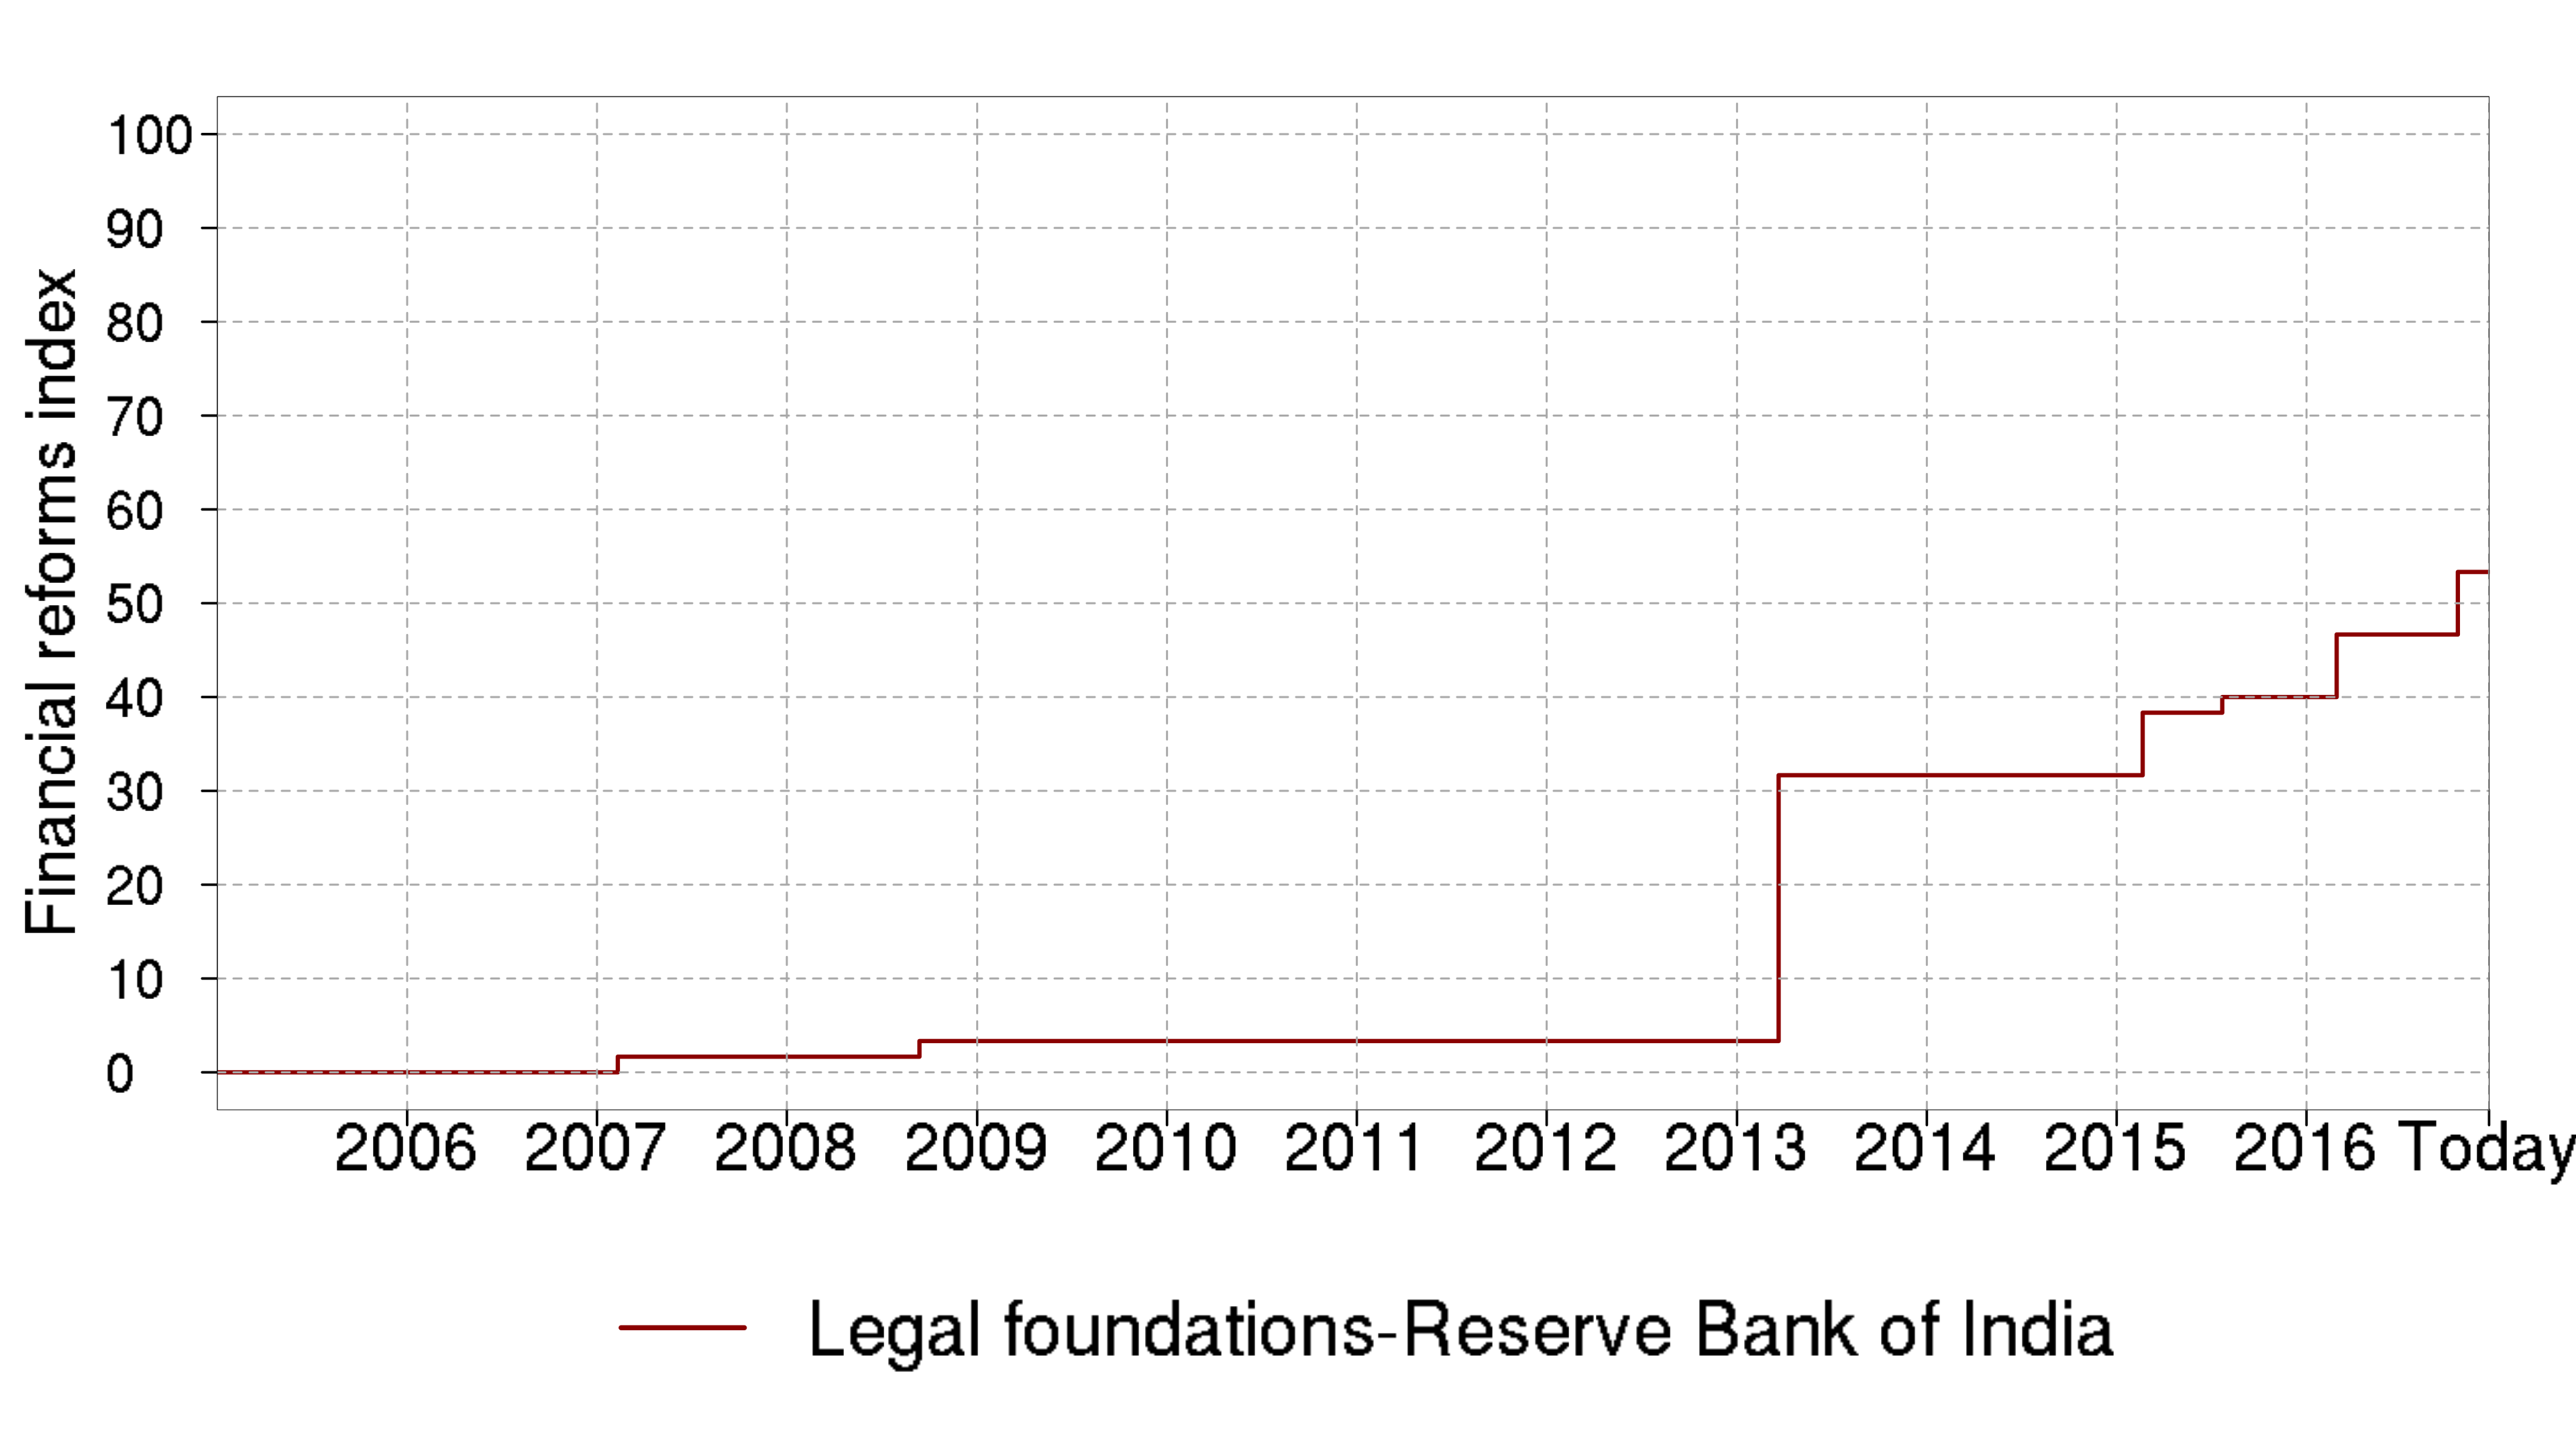
\includegraphics[width=0.65\paperwidth,height=0.45\paperwidth]{../GRAPHS/frm_index_legal_foundations_reserve_bank_of_india.png}
\end{figure}

\newpage
  \begin{table} [H]
    \caption{Legal foundation: Unified financial authority}
    \begin{threeparttable}
      \begin{footnotesize}
        \resizebox{1\textwidth}{!}{
        
          \glfufa{\lfufac}{\lfufadl}{\lfufale}{\lfufali}
        }
      \end{footnotesize}
    \end{threeparttable}
  \end{table}
\begin{figure}[H]
  \caption{Legal foundation: Unified financial authority}

\centering
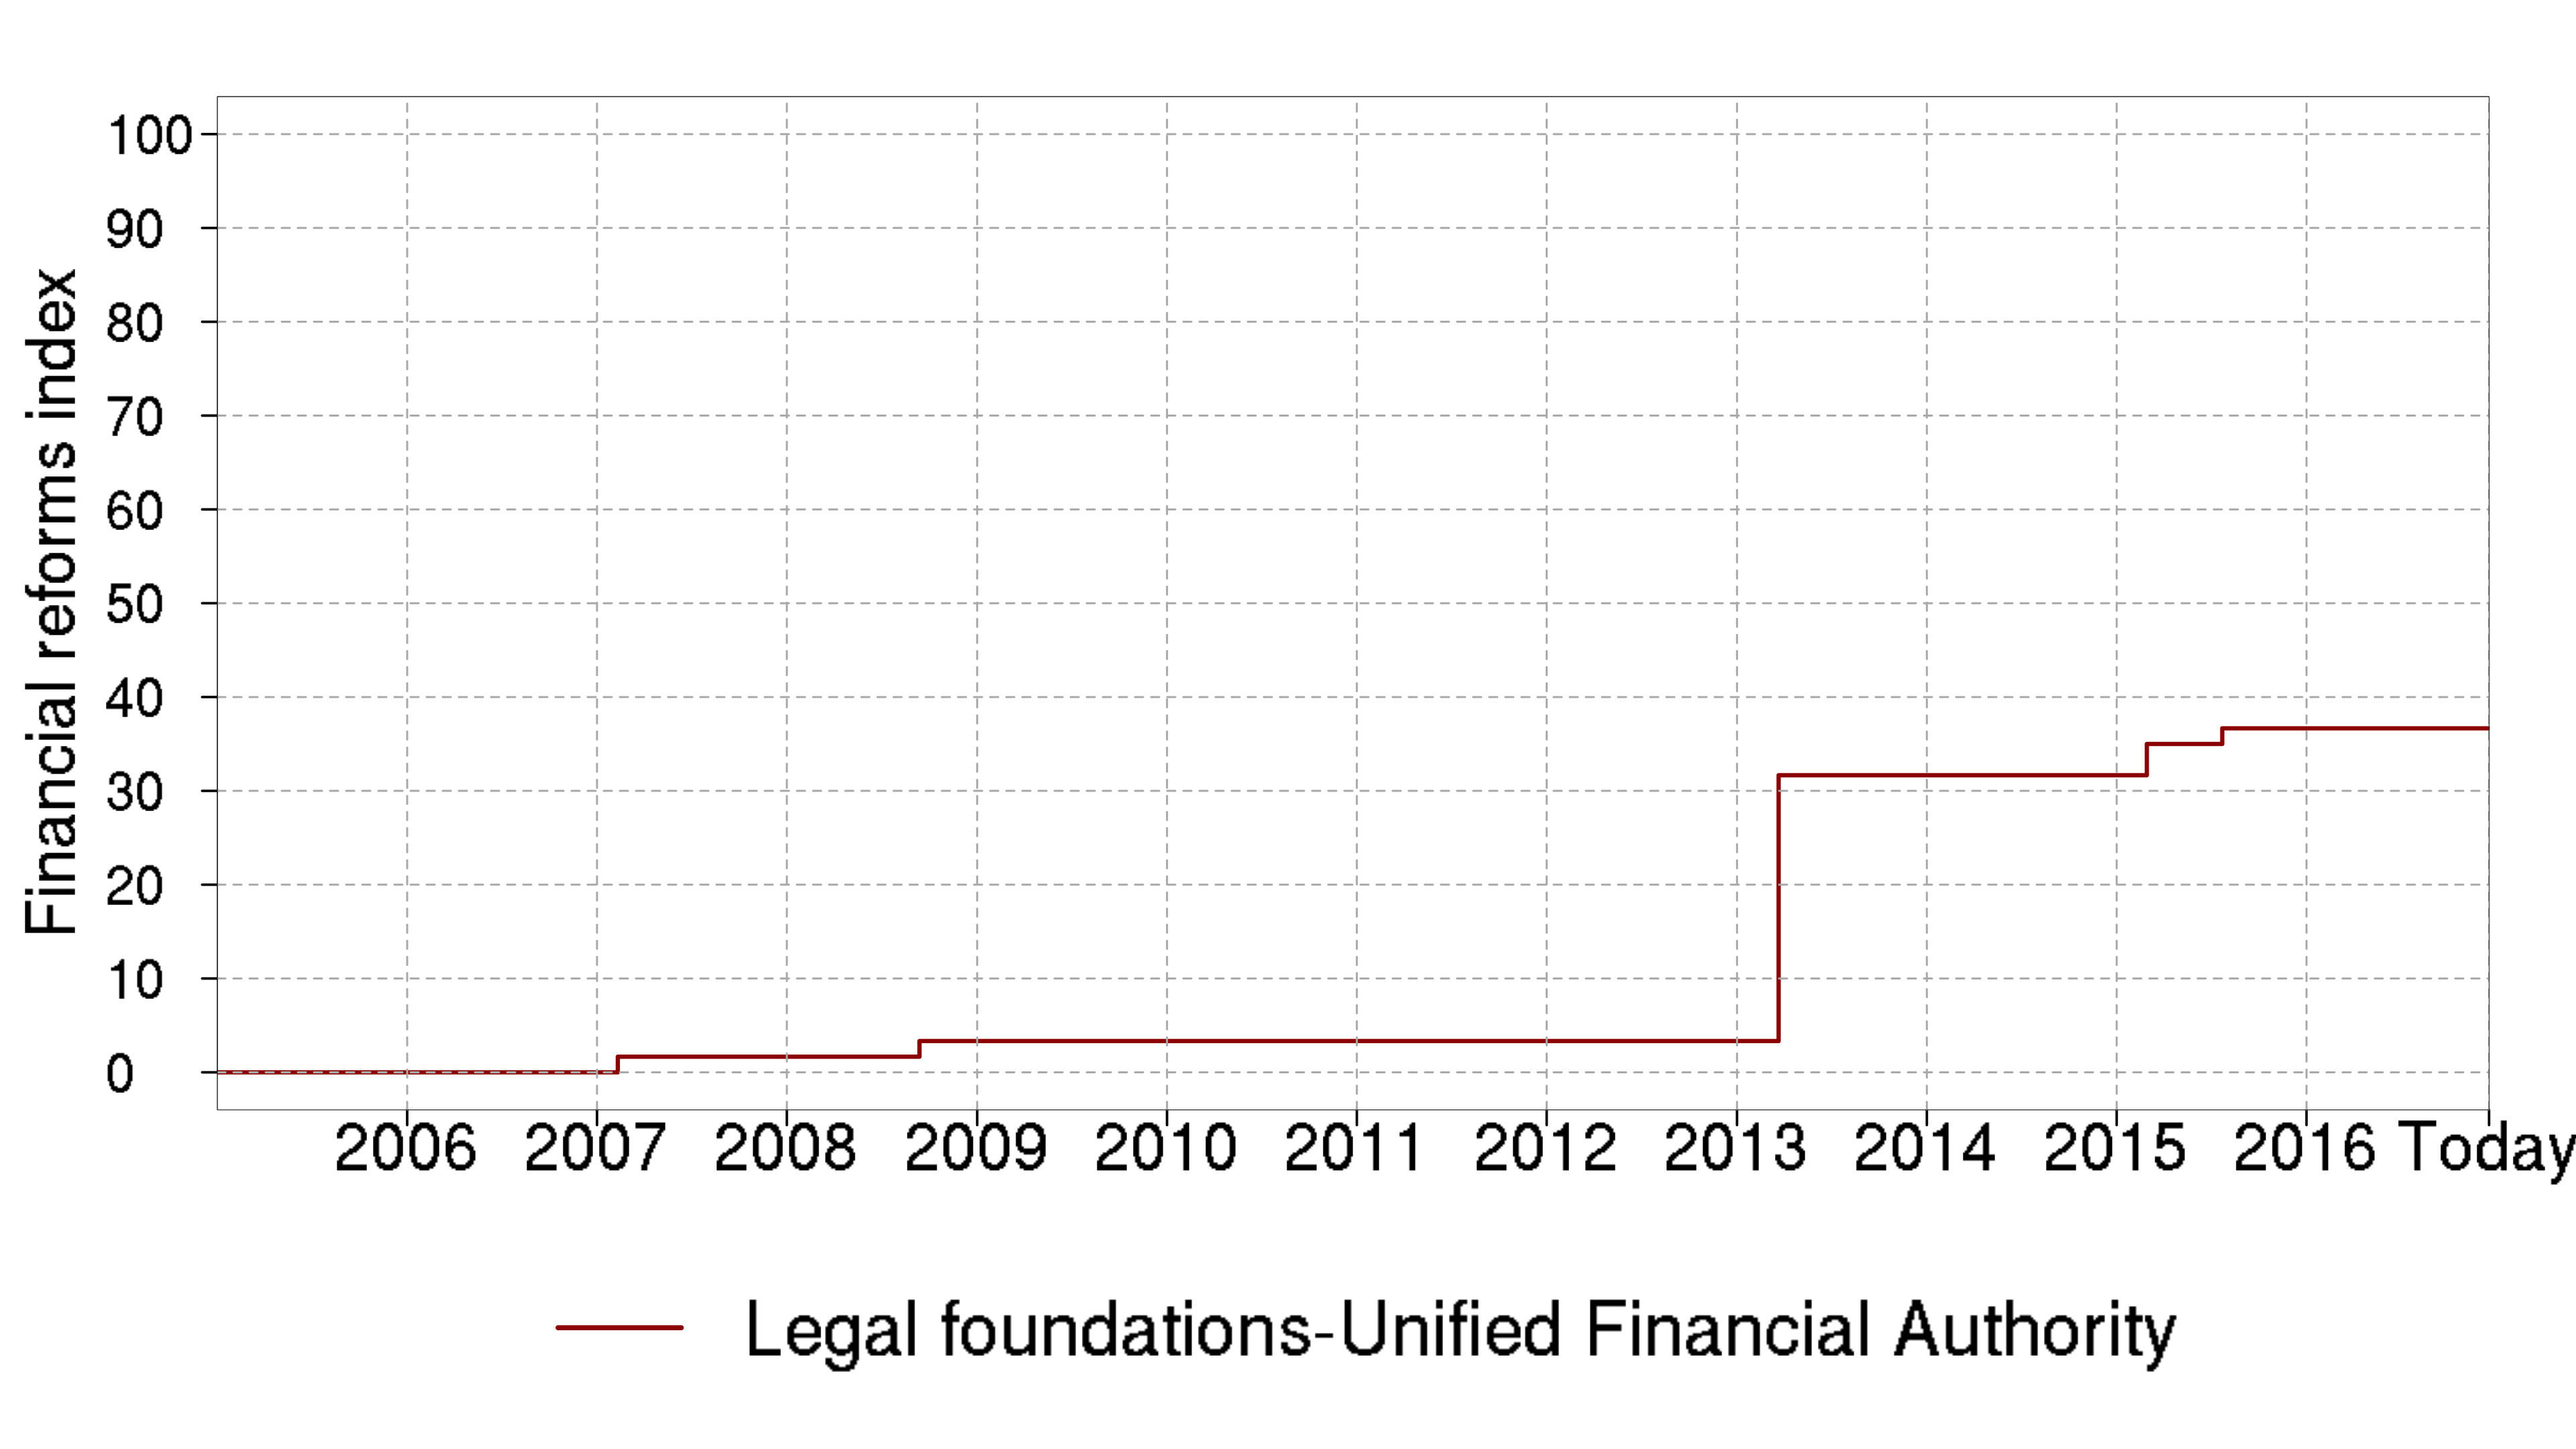
\includegraphics[width=0.65\paperwidth,height=0.45\paperwidth]{../GRAPHS/frm_index_legal_foundations_unified_financial_authority.png}
\end{figure}

\newpage
  \begin{table} [H]
    \caption{Legal foundation: Public debt management agency}
    \begin{threeparttable}
      \begin{footnotesize}
        \resizebox{1\textwidth}{!}{
        
          \glfpdma{\lfpdmac}{\lfpdmadl}{\lfpdmale}{\lfpdmali}
        }
      \end{footnotesize}
    \end{threeparttable}
  \end{table}
\begin{figure}[H]
  \caption{Legal foundation: Public debt management agency}
\centering
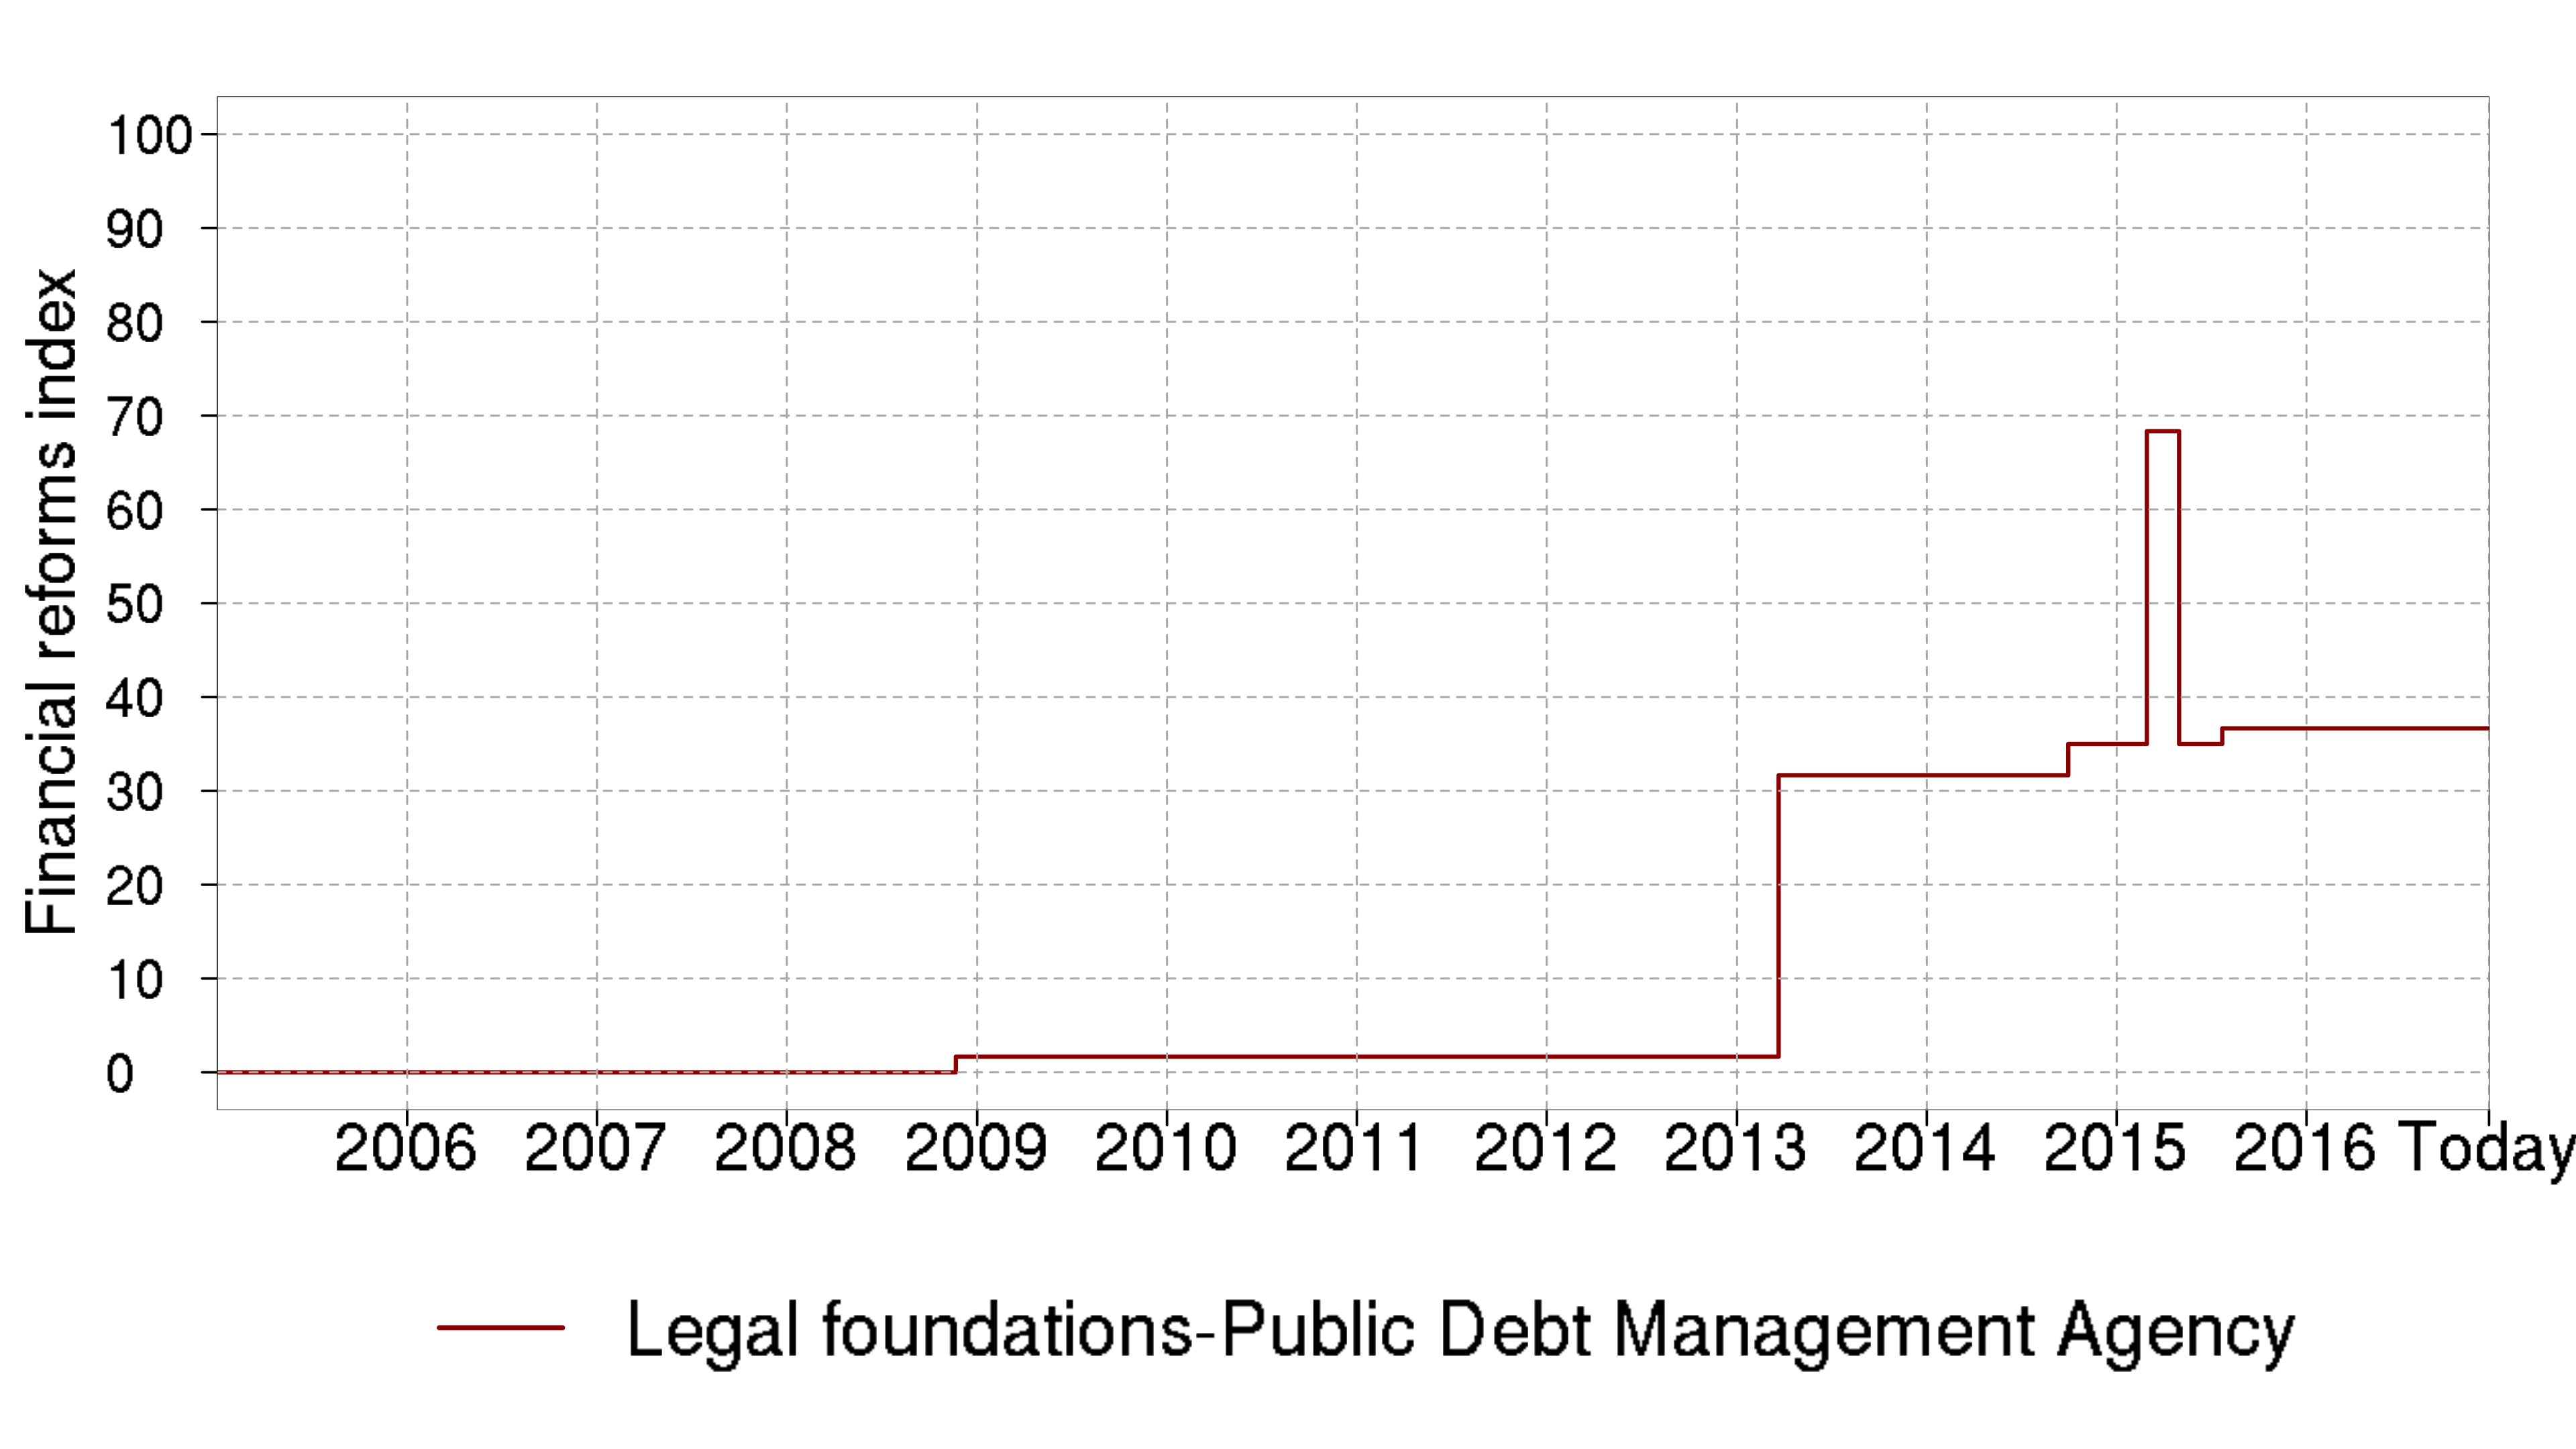
\includegraphics[width=0.65\paperwidth,height=0.45\paperwidth]{../GRAPHS/frm_index_legal_foundations_public_debt_management_agency.png}
\end{figure}

\newpage
  \begin{table} [H]
    \caption{Legal foundation: Financial stability and development council}
    \begin{threeparttable}
      \begin{footnotesize}
        \resizebox{1\textwidth}{!}{
        
          \glffsdc{\lffsdcc}{\lffsdcdl}{\lffsdcle}{\lffsdcli}
        }
      \end{footnotesize}
    \end{threeparttable}
  \end{table}
\begin{figure}[H]
  \caption{Legal foundation: Financial stability and development council}

\centering
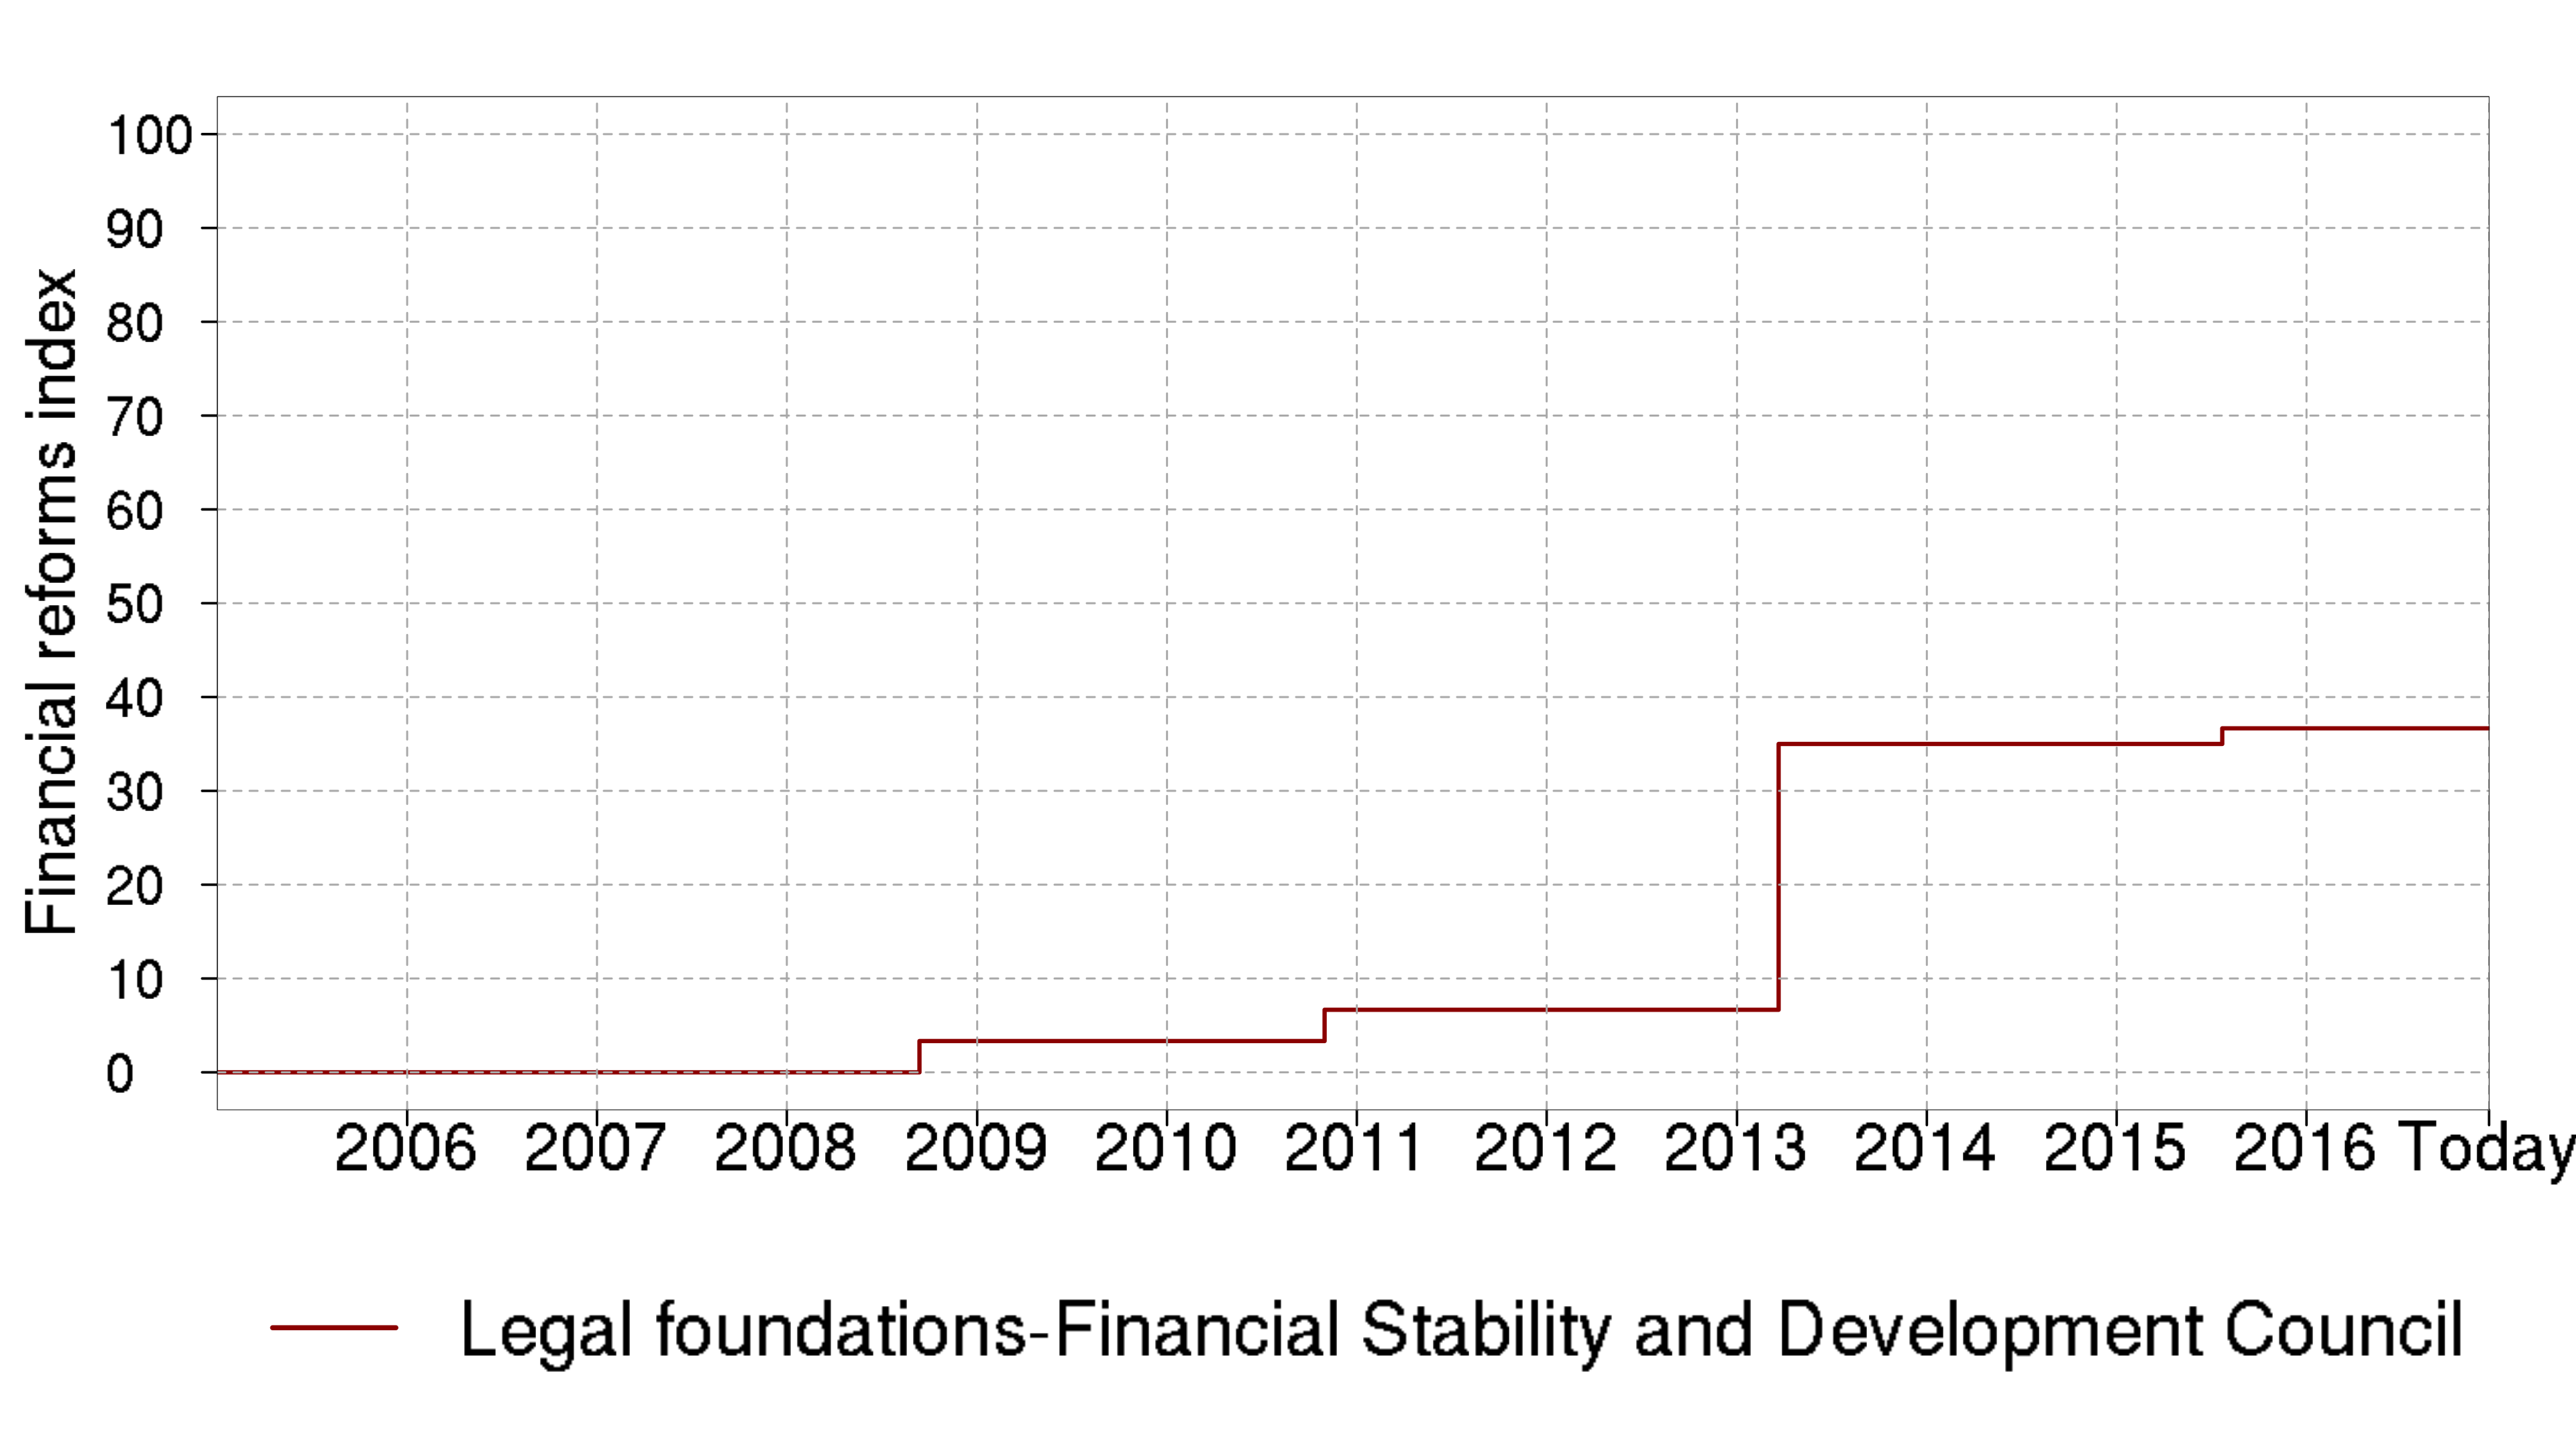
\includegraphics[width=0.65\paperwidth,height=0.45\paperwidth]{../GRAPHS/frm_index_legal_foundations_financial_stability_and_development_council.png}
\end{figure}

\begin{titlepage}
  \vspace*{\stretch{1}}

  \parbox{\textwidthorig}{
  \hrule
  \vspace{\baselineskip} \center{\Large Section index: Legal foundations}
  \vspace{\baselineskip}
  \hrule
  }
  \vspace{\stretch{1}}

  \parbox{\textwidthorig}{
}
\end{titlepage}

\begin{table} [H]
  \caption{Section index: Legal foundations}
  \begin{threeparttable}
    \begin{footnotesize}
      \resizebox{1\textwidth}{!}{
        \glf{\lf}
      }
    \end{footnotesize}
  \end{threeparttable}
\end{table}

\begin{figure}[H]
\caption{Section index: Legal foundations}
\centering
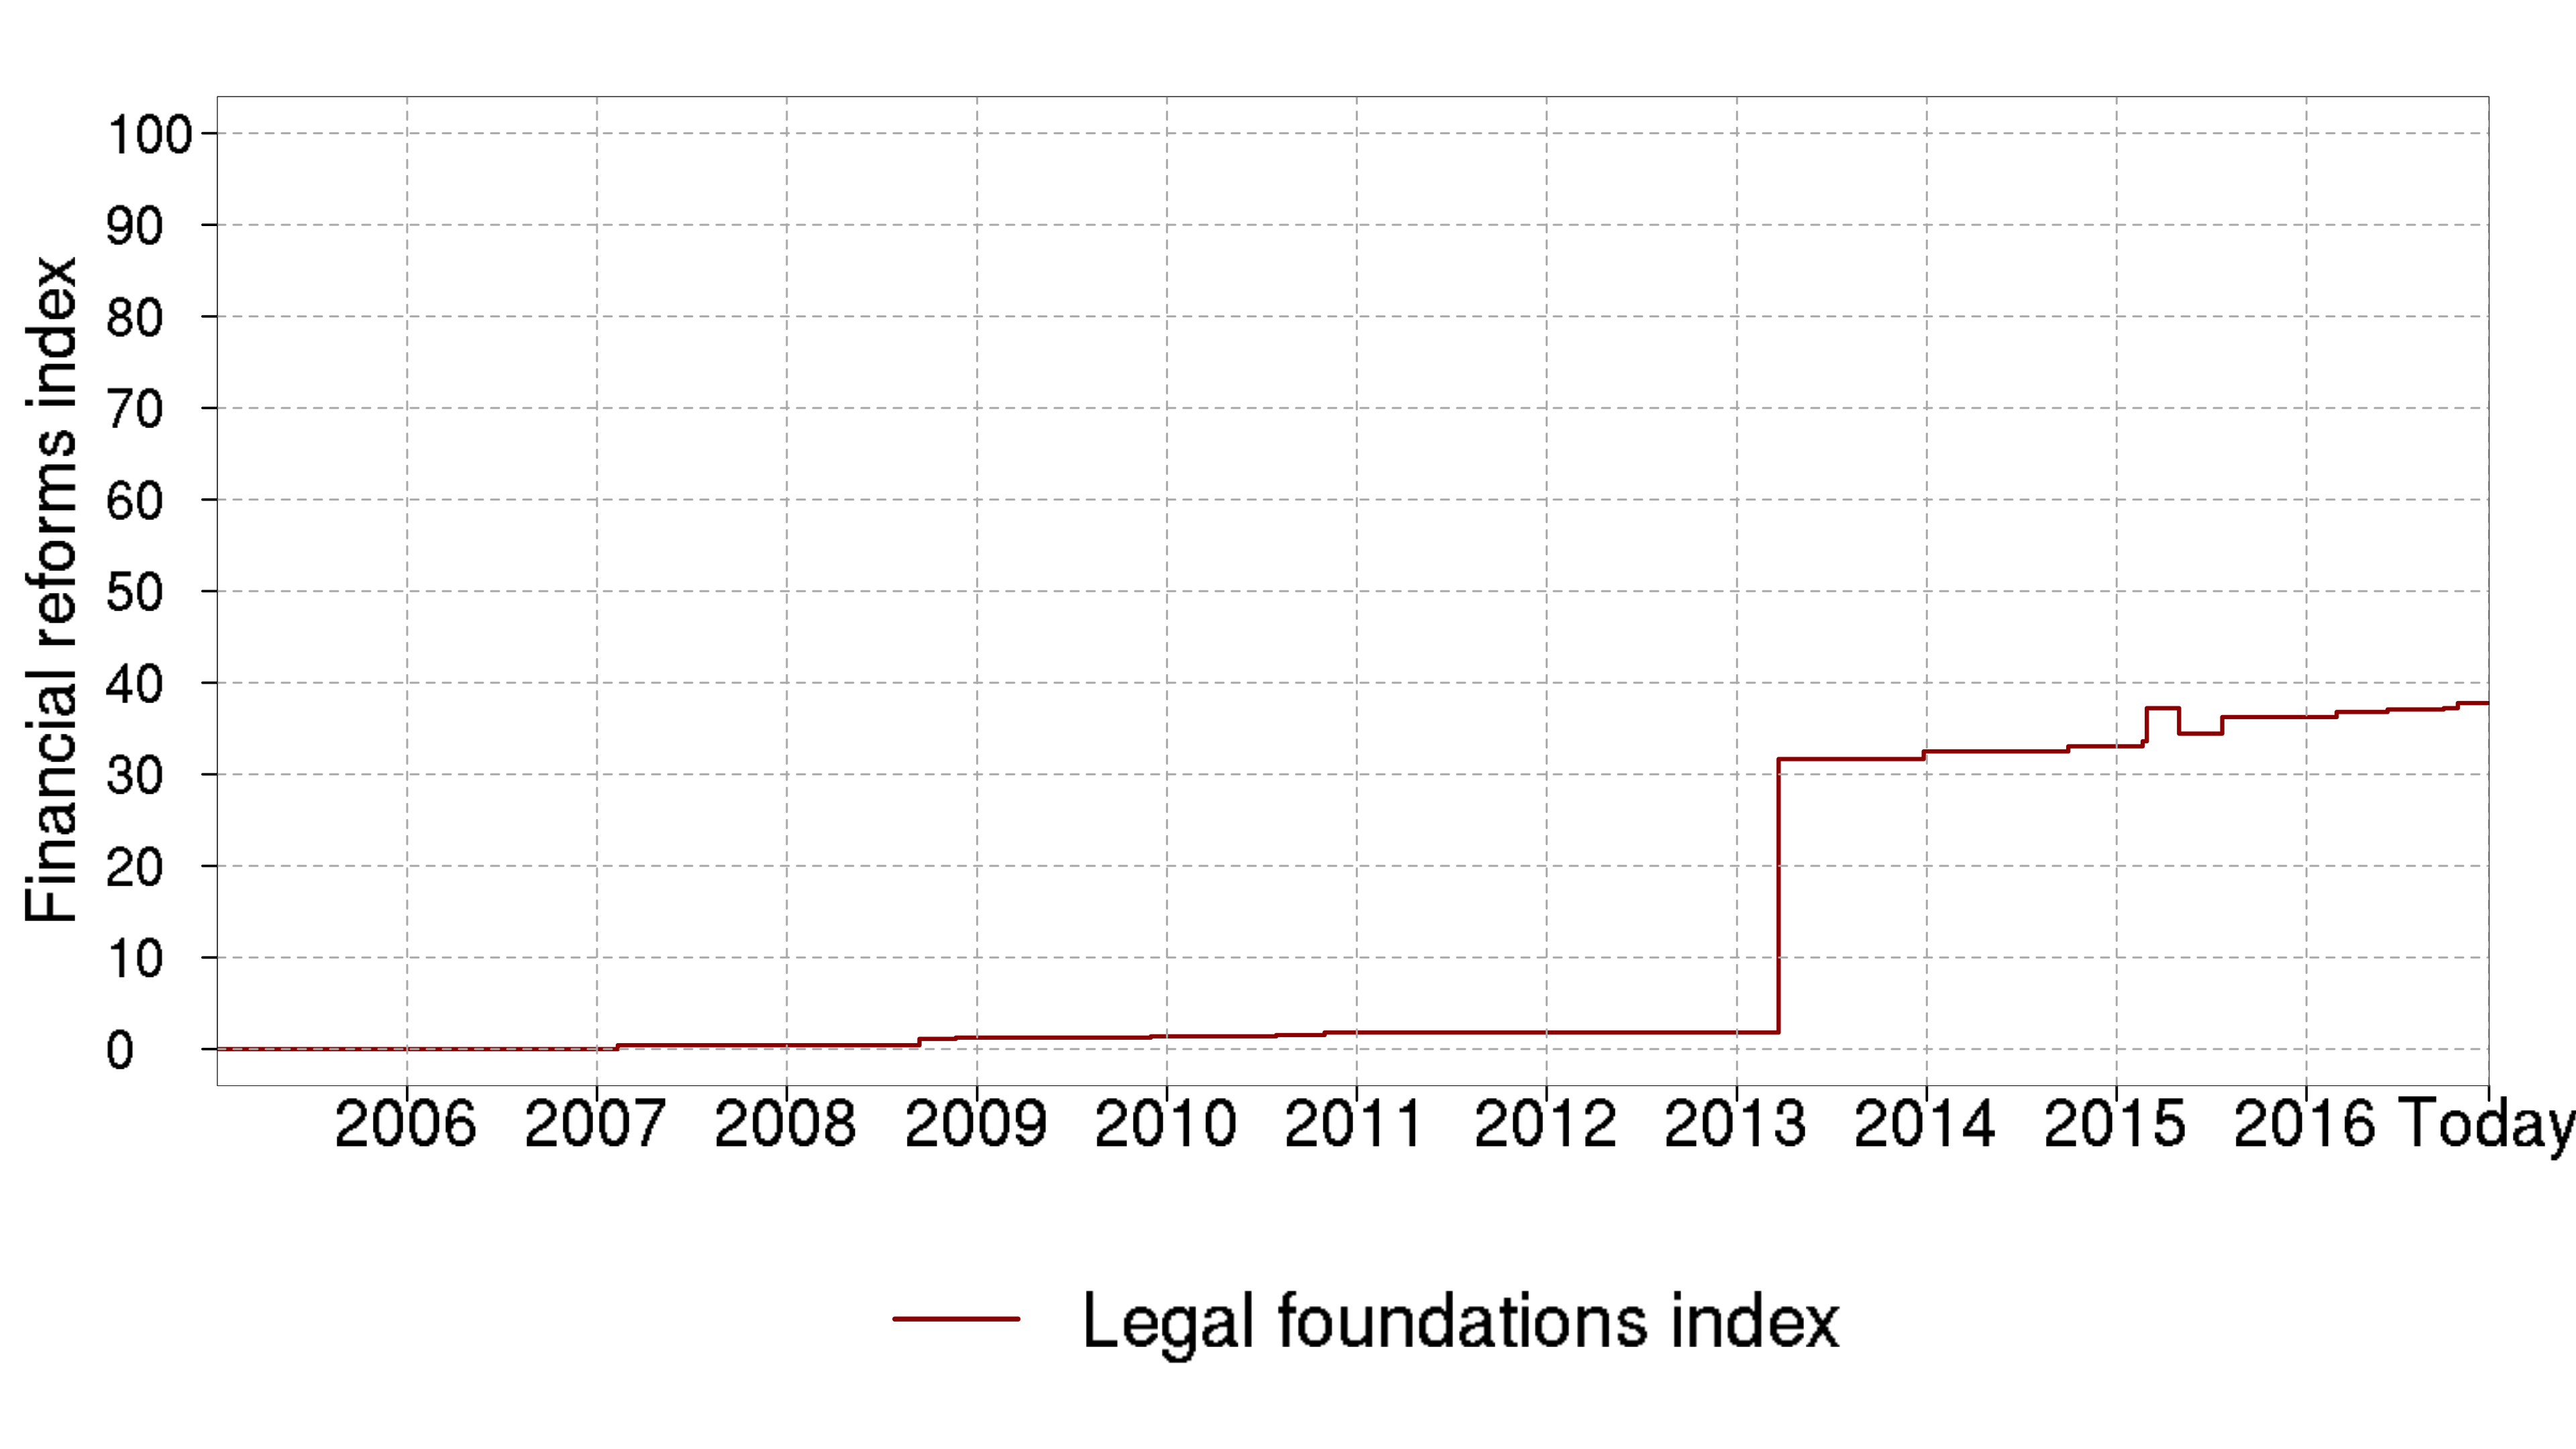
\includegraphics[width=0.9\paperwidth,height=0.7\paperwidth]{../GRAPHS/frm_index_legal_foundations.png}
\end{figure}

\begin{titlepage}
  \vspace*{\stretch{1}}

  \parbox{\textwidthorig}{
  \hrule
  \vspace{\baselineskip} \center{\Large Markets}
  \vspace{\baselineskip}
  \hrule
  }
  \vspace{\stretch{1}}

  \parbox{\textwidthorig}{
}

\end{titlepage}

\refstepcounter{section}
\sectionmark{Markets}
\addcontentsline{toc}{section}{\protect\numberline{\thesection}Markets}

\newpage
  \begin{table} [H]
    \caption{Markets: Equity}
    \begin{threeparttable}
      \begin{footnotesize}
        \resizebox{1\textwidth}{!}{
          \begin{tabular} {ABCDE}%{p{1.5cm}p{1.5cm}p{5cm}p{5cm}p{1cm}}
            \hline
            \noalign{\vskip .09in}
            \multicolumn{5}{p{7in}}{\textbf{\small{Markets:}}} \\ \hline
            \noalign{\vskip .06in}
            \multicolumn{5}{p{7in}}{\textbf{\textit{\footnotesize{Equity:}}}} \\ \hline
            \noalign{\vskip .01in}
            \multicolumn{3}{c}{\textbf{\underline{\footnotesize{Market Infrastructure}}}} & \multicolumn{2}{c}{\textbf{\footnotesize{\colorbox{lightgray}{weight: 20}}}}  \\ \hline  
            \noalign{\vskip .06in}
            \textbf{Date} & \textbf{Milestone} & \textbf{URL} & \textbf{Story} & \textbf{Score} \\ \hline
            \input{../TABLES/markets_equities_marketinfrastructure.tex}
            \hline
            \noalign{\vskip .06in}
            \multicolumn{3}{c}{\textbf{\underline{\footnotesize{Entry Barriers into inter-mediation}}}} & \multicolumn{2}{c}{\textbf{\footnotesize{\colorbox{lightgray}{weight: 20}}}}  \\ \hline
            \noalign{\vskip .01in}
            \textbf{Date} & \textbf{Milestone} & \textbf{URL} & \textbf{Story} & \textbf{Score} \\ \hline
            \input{../TABLES/markets_equities_entrybarriersintointermediation.tex}
            \hline
            \noalign{\vskip .06in}
            \multicolumn{3}{c}{\textbf{\underline{\footnotesize{Sound regulatory arrangement}}}} & \multicolumn{2}{c}{\textbf{\footnotesize{\colorbox{lightgray}{weight:20}}}}  \\ \hline
            \noalign{\vskip .01in}
            \textbf{Date} & \textbf{Milestone} & \textbf{URL} & \textbf{Story} & \textbf{Score} \\ \hline
            \input{../TABLES/markets_equities_soundregulatoryarrangement.tex}
            \hline
            \noalign{\vskip .06in}
            \multicolumn{3}{c}{\textbf{\underline{\footnotesize{Sound regulations}}}} & \multicolumn{2}{c}{\textbf{\footnotesize{\colorbox{lightgray}{weight:20}}}}  \\ \hline
            \noalign{\vskip .01in}
            \textbf{Date} & \textbf{Milestone} & \textbf{URL} & \textbf{Story} & \textbf{Score} \\ \hline
            \input{../TABLES/markets_equities_soundregulations.tex}
            \hline
            \noalign{\vskip .06in}
            \hline
            \multicolumn{3}{c}{\textbf{\underline{\footnotesize{Enforcement of regulations}}}} & \multicolumn{2}{c}{\textbf{\footnotesize{\colorbox{lightgray}{weight:20}}}}  \\ \hline
            \noalign{\vskip .01in}
            \textbf{Date} & \textbf{Milestone} & \textbf{URL} & \textbf{Story} & \textbf{Score} \\ \hline
            \input{../TABLES/markets_equities_enforcementofregulations.tex}
            \hline
            \noalign{\vskip .06in}
            \hline
            
            \multicolumn{5}{p{6in}}{\textit{\scriptsize{Explanation:
    Financial reforms for equity markets.}}}
  \end{tabular}
}
      \end{footnotesize}
    \end{threeparttable}
  \end{table}
\begin{figure}[H]
  \caption{Markets: Equity}
\centering
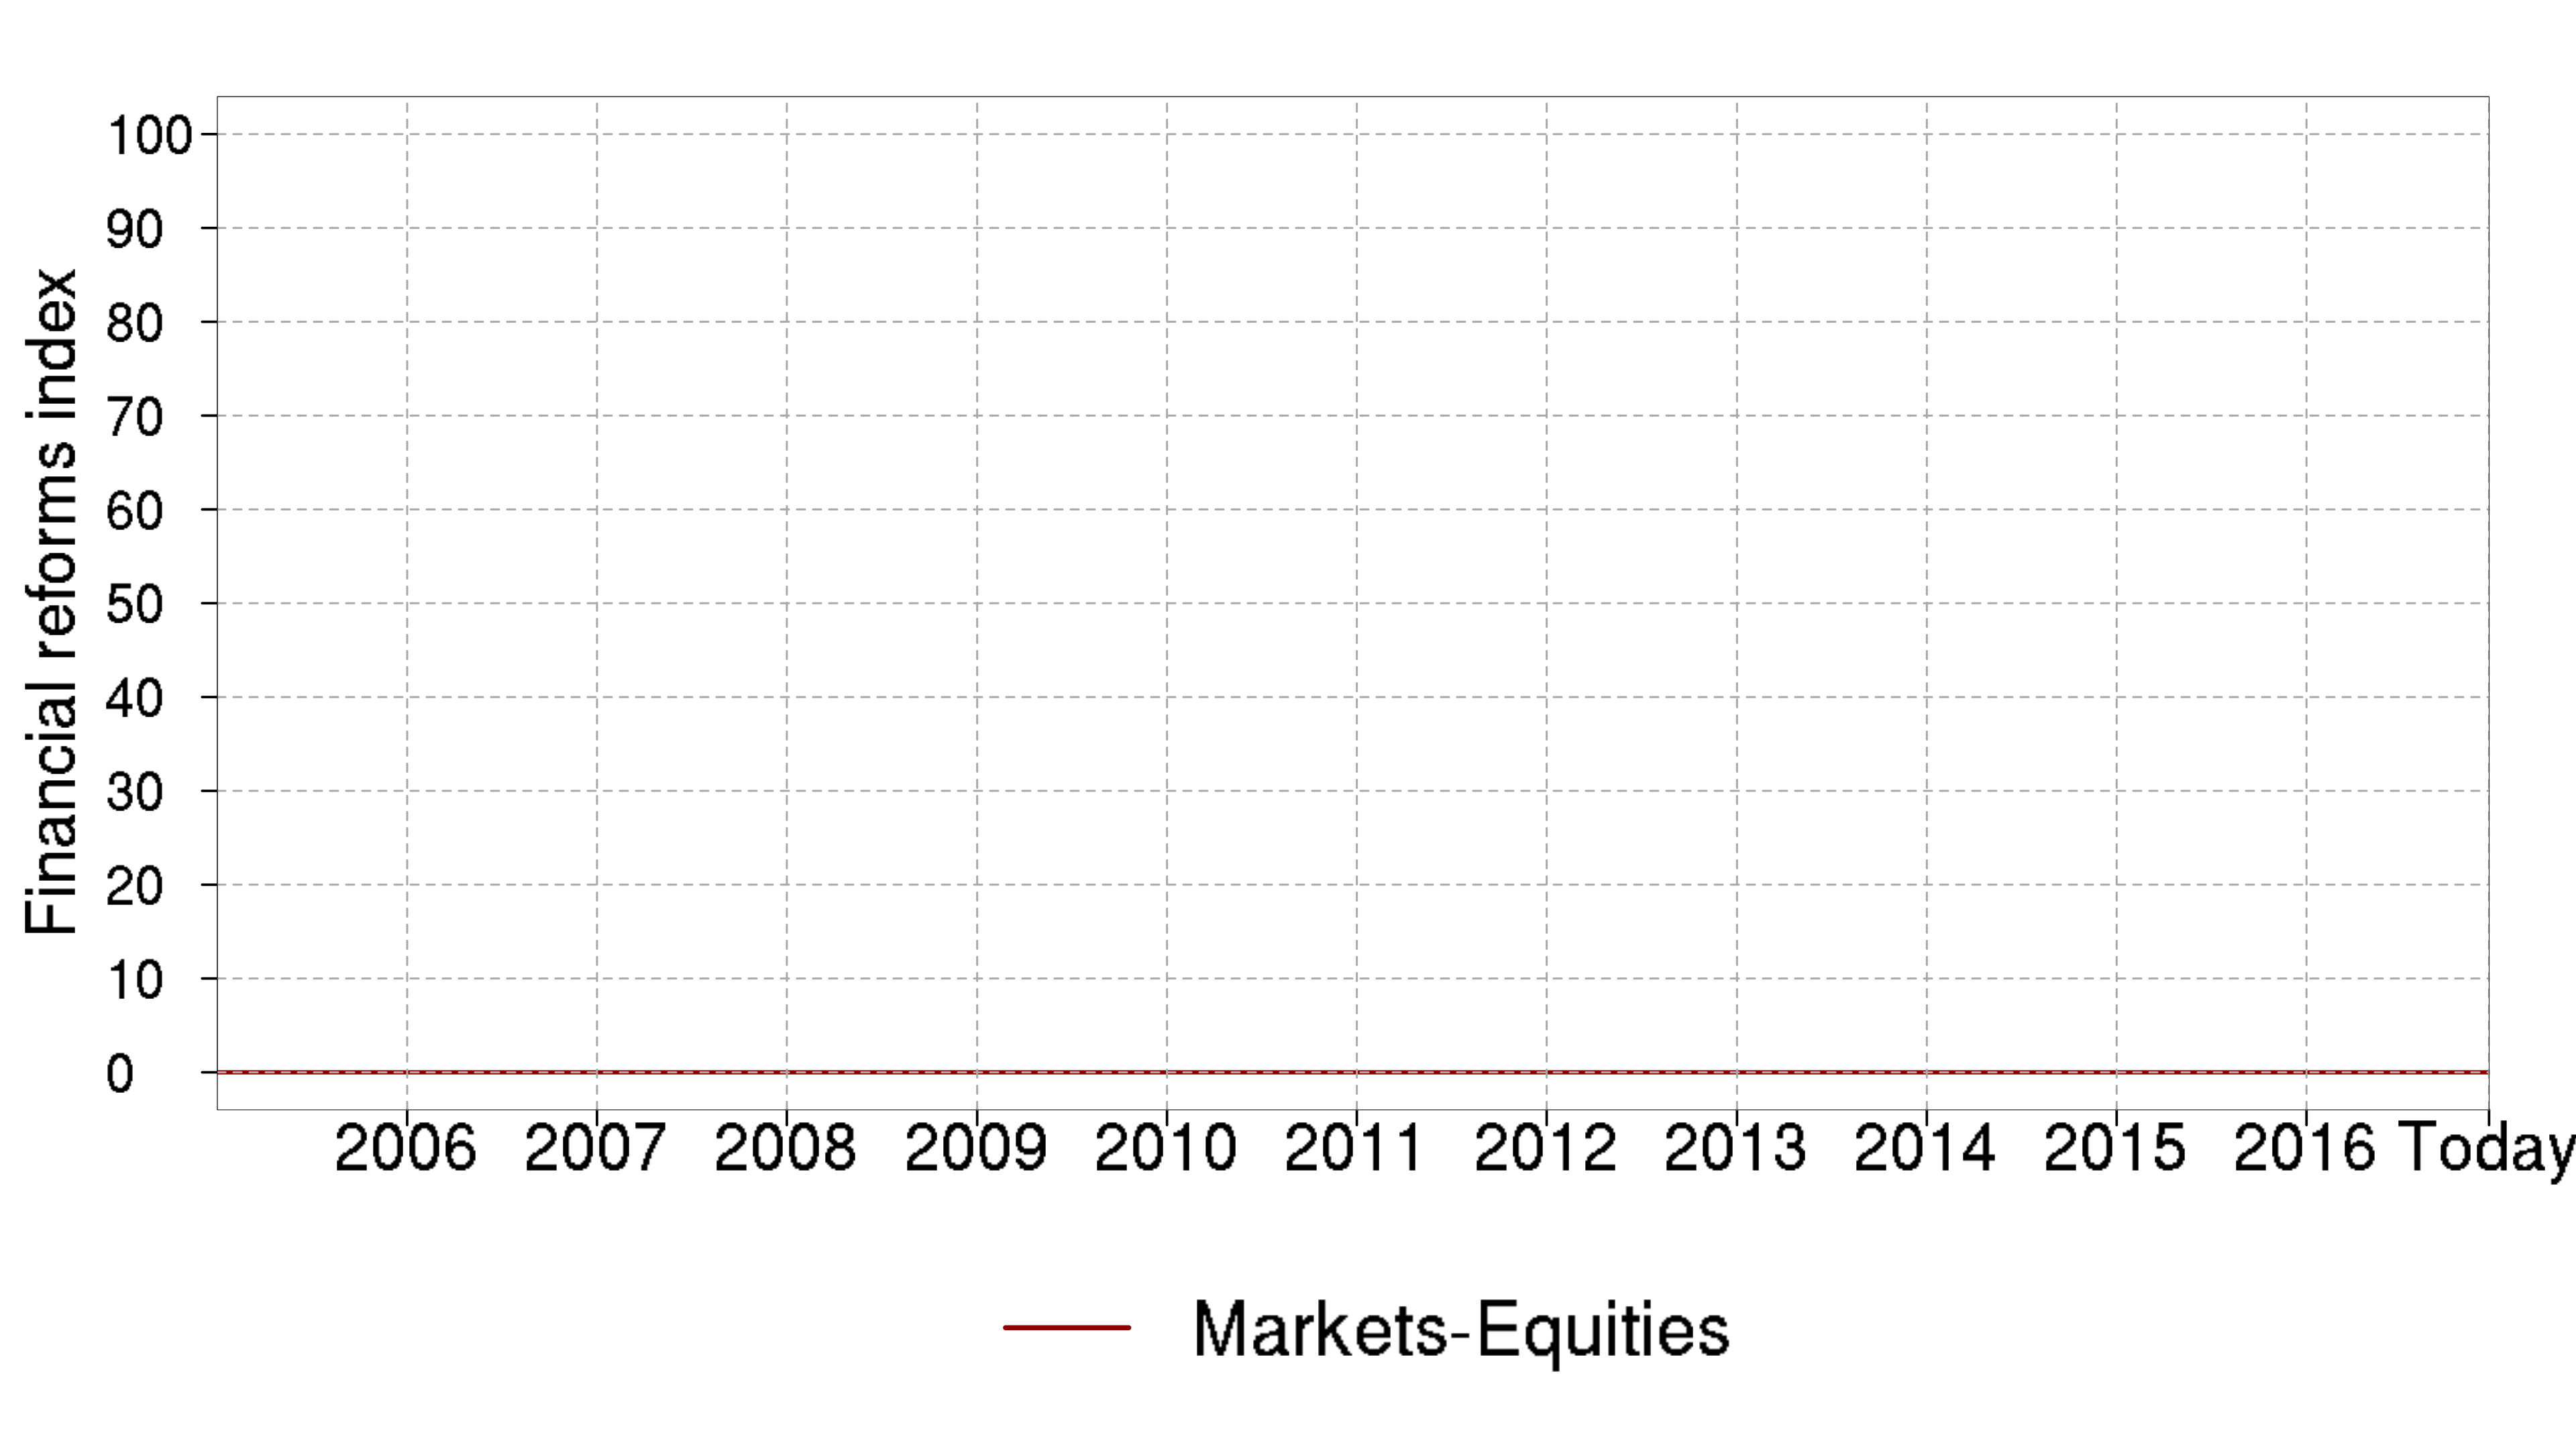
\includegraphics[width=0.65\paperwidth,height=0.45\paperwidth]{../GRAPHS/frm_index_markets_equities.png}
\end{figure}

\newpage

  \begin{table} [H]
    \caption{Markets: BCD Nexus}
    \begin{threeparttable}
      \begin{footnotesize}
        \resizebox{1\textwidth}{!}{
          \begin{tabular} {ABCDE}%{p{1.5cm}p{1.5cm}p{5cm}p{5cm}p{1cm}}
            \hline
            \noalign{\vskip .09in}
            \multicolumn{5}{p{7in}}{\textbf{\small{Markets:}}} \\ \hline
            \noalign{\vskip .06in}
            \multicolumn{5}{p{7in}}{\textbf{\textit{\footnotesize{BCD Nexus:}}}} \\ \hline
            \noalign{\vskip .01in}
            \multicolumn{3}{c}{\textbf{\underline{\footnotesize{Market Infrastructure}}}} & \multicolumn{2}{c}{\textbf{\footnotesize{\colorbox{lightgray}{weight: 20}}}}  \\ \hline  
            \noalign{\vskip .06in}
            \textbf{Date} & \textbf{Milestone} & \textbf{URL} & \textbf{Story} & \textbf{Score} \\ \hline
            \input{../TABLES/markets_bcd_nexus_marketinfrastructure.tex}
            \hline
            \noalign{\vskip .06in}
            \multicolumn{3}{c}{\textbf{\underline{\footnotesize{Entry Barriers into inter-mediation}}}} & \multicolumn{2}{c}{\textbf{\footnotesize{\colorbox{lightgray}{weight: 20}}}}  \\ \hline
            \noalign{\vskip .01in}
            \textbf{Date} & \textbf{Milestone} & \textbf{URL} & \textbf{Story} & \textbf{Score} \\ \hline
            \input{../TABLES/markets_bcd_nexus_entrybarriersintointermediation.tex}
            \hline
            \noalign{\vskip .06in}
            \multicolumn{3}{c}{\textbf{\underline{\footnotesize{Sound regulatory arrangement}}}} & \multicolumn{2}{c}{\textbf{\footnotesize{\colorbox{lightgray}{weight:20}}}}  \\ \hline
            \noalign{\vskip .01in}
            \textbf{Date} & \textbf{Milestone} & \textbf{URL} & \textbf{Story} & \textbf{Score} \\ \hline
            \input{../TABLES/markets_bcd_nexus_soundregulatoryarrangement.tex}
            \hline
            \noalign{\vskip .06in}
            \multicolumn{3}{c}{\textbf{\underline{\footnotesize{Sound regulations}}}} & \multicolumn{2}{c}{\textbf{\footnotesize{\colorbox{lightgray}{weight:20}}}}  \\ \hline
            \noalign{\vskip .01in}
            \textbf{Date} & \textbf{Milestone} & \textbf{URL} & \textbf{Story} & \textbf{Score} \\ \hline
            \input{../TABLES/markets_bcd_nexus_soundregulations.tex}
            \hline
            \noalign{\vskip .06in}
            \hline
            \multicolumn{3}{c}{\textbf{\underline{\footnotesize{Enforcement of regulations}}}} & \multicolumn{2}{c}{\textbf{\footnotesize{\colorbox{lightgray}{weight:20}}}}  \\ \hline
            \noalign{\vskip .01in}
            \textbf{Date} & \textbf{Milestone} & \textbf{URL} & \textbf{Story} & \textbf{Score} \\ \hline
            \input{../TABLES/markets_bcd_nexus_enforcementofregulations.tex}
            \hline
            \noalign{\vskip .06in}
            \hline
            
            \multicolumn{5}{p{6in}}{\textit{\scriptsize{Explanation:
    Financial reforms for bond markets.}}}
  \end{tabular}
}
\end{footnotesize}
\end{threeparttable}
\end{table}
\begin{figure}[H]
  \caption{Markets: BCD Nexus}
  \centering
  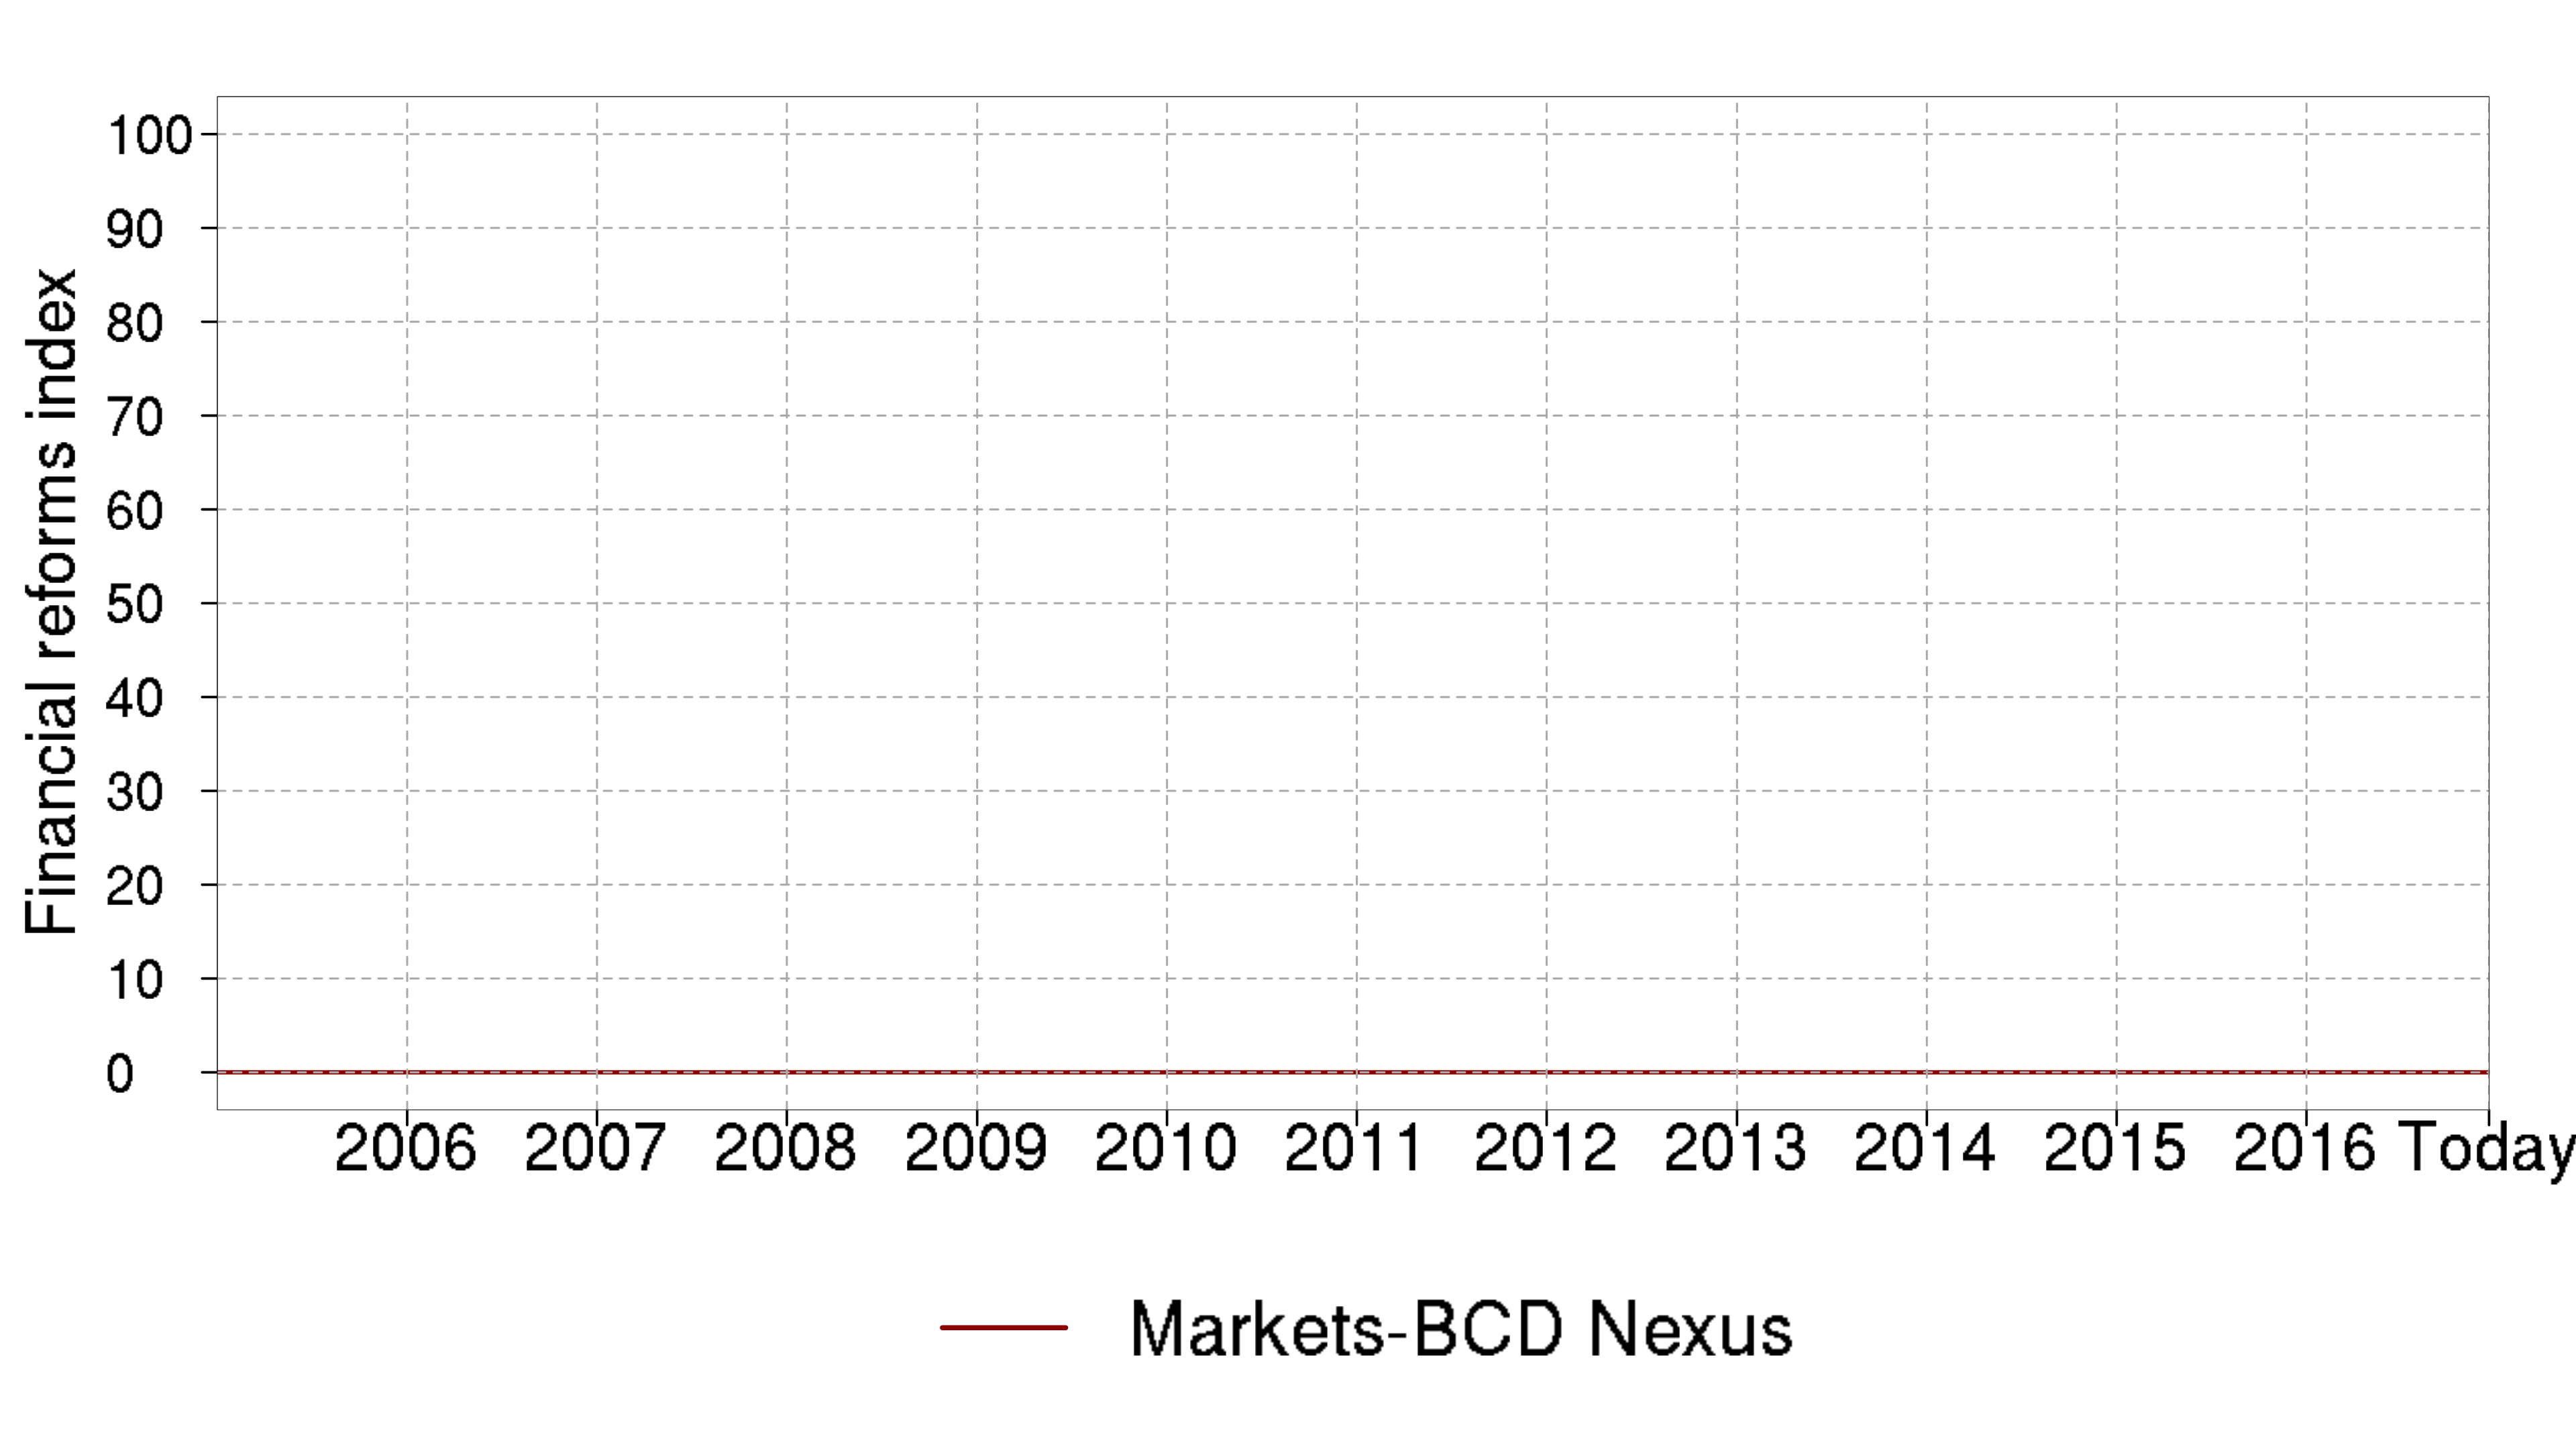
\includegraphics[width=0.65\paperwidth,height=0.45\paperwidth]{../GRAPHS/frm_index_markets_bcd_nexus.png}
\end{figure}

\newpage
  \begin{table} [H]
    \caption{Markets: Commodities}
    \begin{threeparttable}
      \begin{footnotesize}
        \resizebox{1\textwidth}{!}{
          \begin{tabular} {ABCDE}%{p{1.5cm}p{1.5cm}p{5cm}p{5cm}p{1cm}}
            \hline
            \noalign{\vskip .09in}
            \multicolumn{5}{p{7in}}{\textbf{\small{Markets:}}} \\ \hline
            \noalign{\vskip .06in}
            \multicolumn{5}{p{7in}}{\textbf{\textit{\footnotesize{Commodities:}}}} \\ \hline
            \noalign{\vskip .01in}
            \multicolumn{3}{c}{\textbf{\underline{\footnotesize{Market Infrastructure}}}} & \multicolumn{2}{c}{\textbf{\footnotesize{\colorbox{lightgray}{weight: 20}}}}  \\ \hline  
            \noalign{\vskip .06in}
            \textbf{Date} & \textbf{Milestone} & \textbf{URL} & \textbf{Story} & \textbf{Score} \\ \hline
            \input{../TABLES/markets_commodities_marketinfrastructure.tex}
            \hline
            \noalign{\vskip .06in}
            \multicolumn{3}{c}{\textbf{\underline{\footnotesize{Entry Barriers into inter-mediation}}}} & \multicolumn{2}{c}{\textbf{\footnotesize{\colorbox{lightgray}{weight: 20}}}}  \\ \hline
            \noalign{\vskip .01in}
            \textbf{Date} & \textbf{Milestone} & \textbf{URL} & \textbf{Story} & \textbf{Score} \\ \hline
            \input{../TABLES/markets_commodities_entrybarriersintointermediation.tex}
            \hline
            \noalign{\vskip .06in}
            \multicolumn{3}{c}{\textbf{\underline{\footnotesize{Sound regulatory arrangement}}}} & \multicolumn{2}{c}{\textbf{\footnotesize{\colorbox{lightgray}{weight:20}}}}  \\ \hline
            \noalign{\vskip .01in}
            \textbf{Date} & \textbf{Milestone} & \textbf{URL} & \textbf{Story} & \textbf{Score} \\ \hline
            \input{../TABLES/markets_commodities_soundregulatoryarrangement.tex}
            \hline
            \noalign{\vskip .06in}
            \multicolumn{3}{c}{\textbf{\underline{\footnotesize{Sound regulations}}}} & \multicolumn{2}{c}{\textbf{\footnotesize{\colorbox{lightgray}{weight:20}}}}  \\ \hline
            \noalign{\vskip .01in}
            \textbf{Date} & \textbf{Milestone} & \textbf{URL} & \textbf{Story} & \textbf{Score} \\ \hline
            \input{../TABLES/markets_commodities_soundregulations.tex}
            \hline
            \noalign{\vskip .06in}
            \hline
            \multicolumn{3}{c}{\textbf{\underline{\footnotesize{Enforcement of regulations}}}} & \multicolumn{2}{c}{\textbf{\footnotesize{\colorbox{lightgray}{weight:20}}}}  \\ \hline
            \noalign{\vskip .01in}
            \textbf{Date} & \textbf{Milestone} & \textbf{URL} & \textbf{Story} & \textbf{Score} \\ \hline
            \input{../TABLES/markets_commodities_enforcementofregulations.tex}
            \hline
            \noalign{\vskip .06in}
            \hline
            
            \multicolumn{5}{p{6in}}{\textit{\scriptsize{Explanation:
            Financial reforms for commodity's markets.}}}
  \end{tabular}
}
      \end{footnotesize}
    \end{threeparttable}
  \end{table}
\begin{figure}[H]
  \caption{Markets: Commodities}
\centering
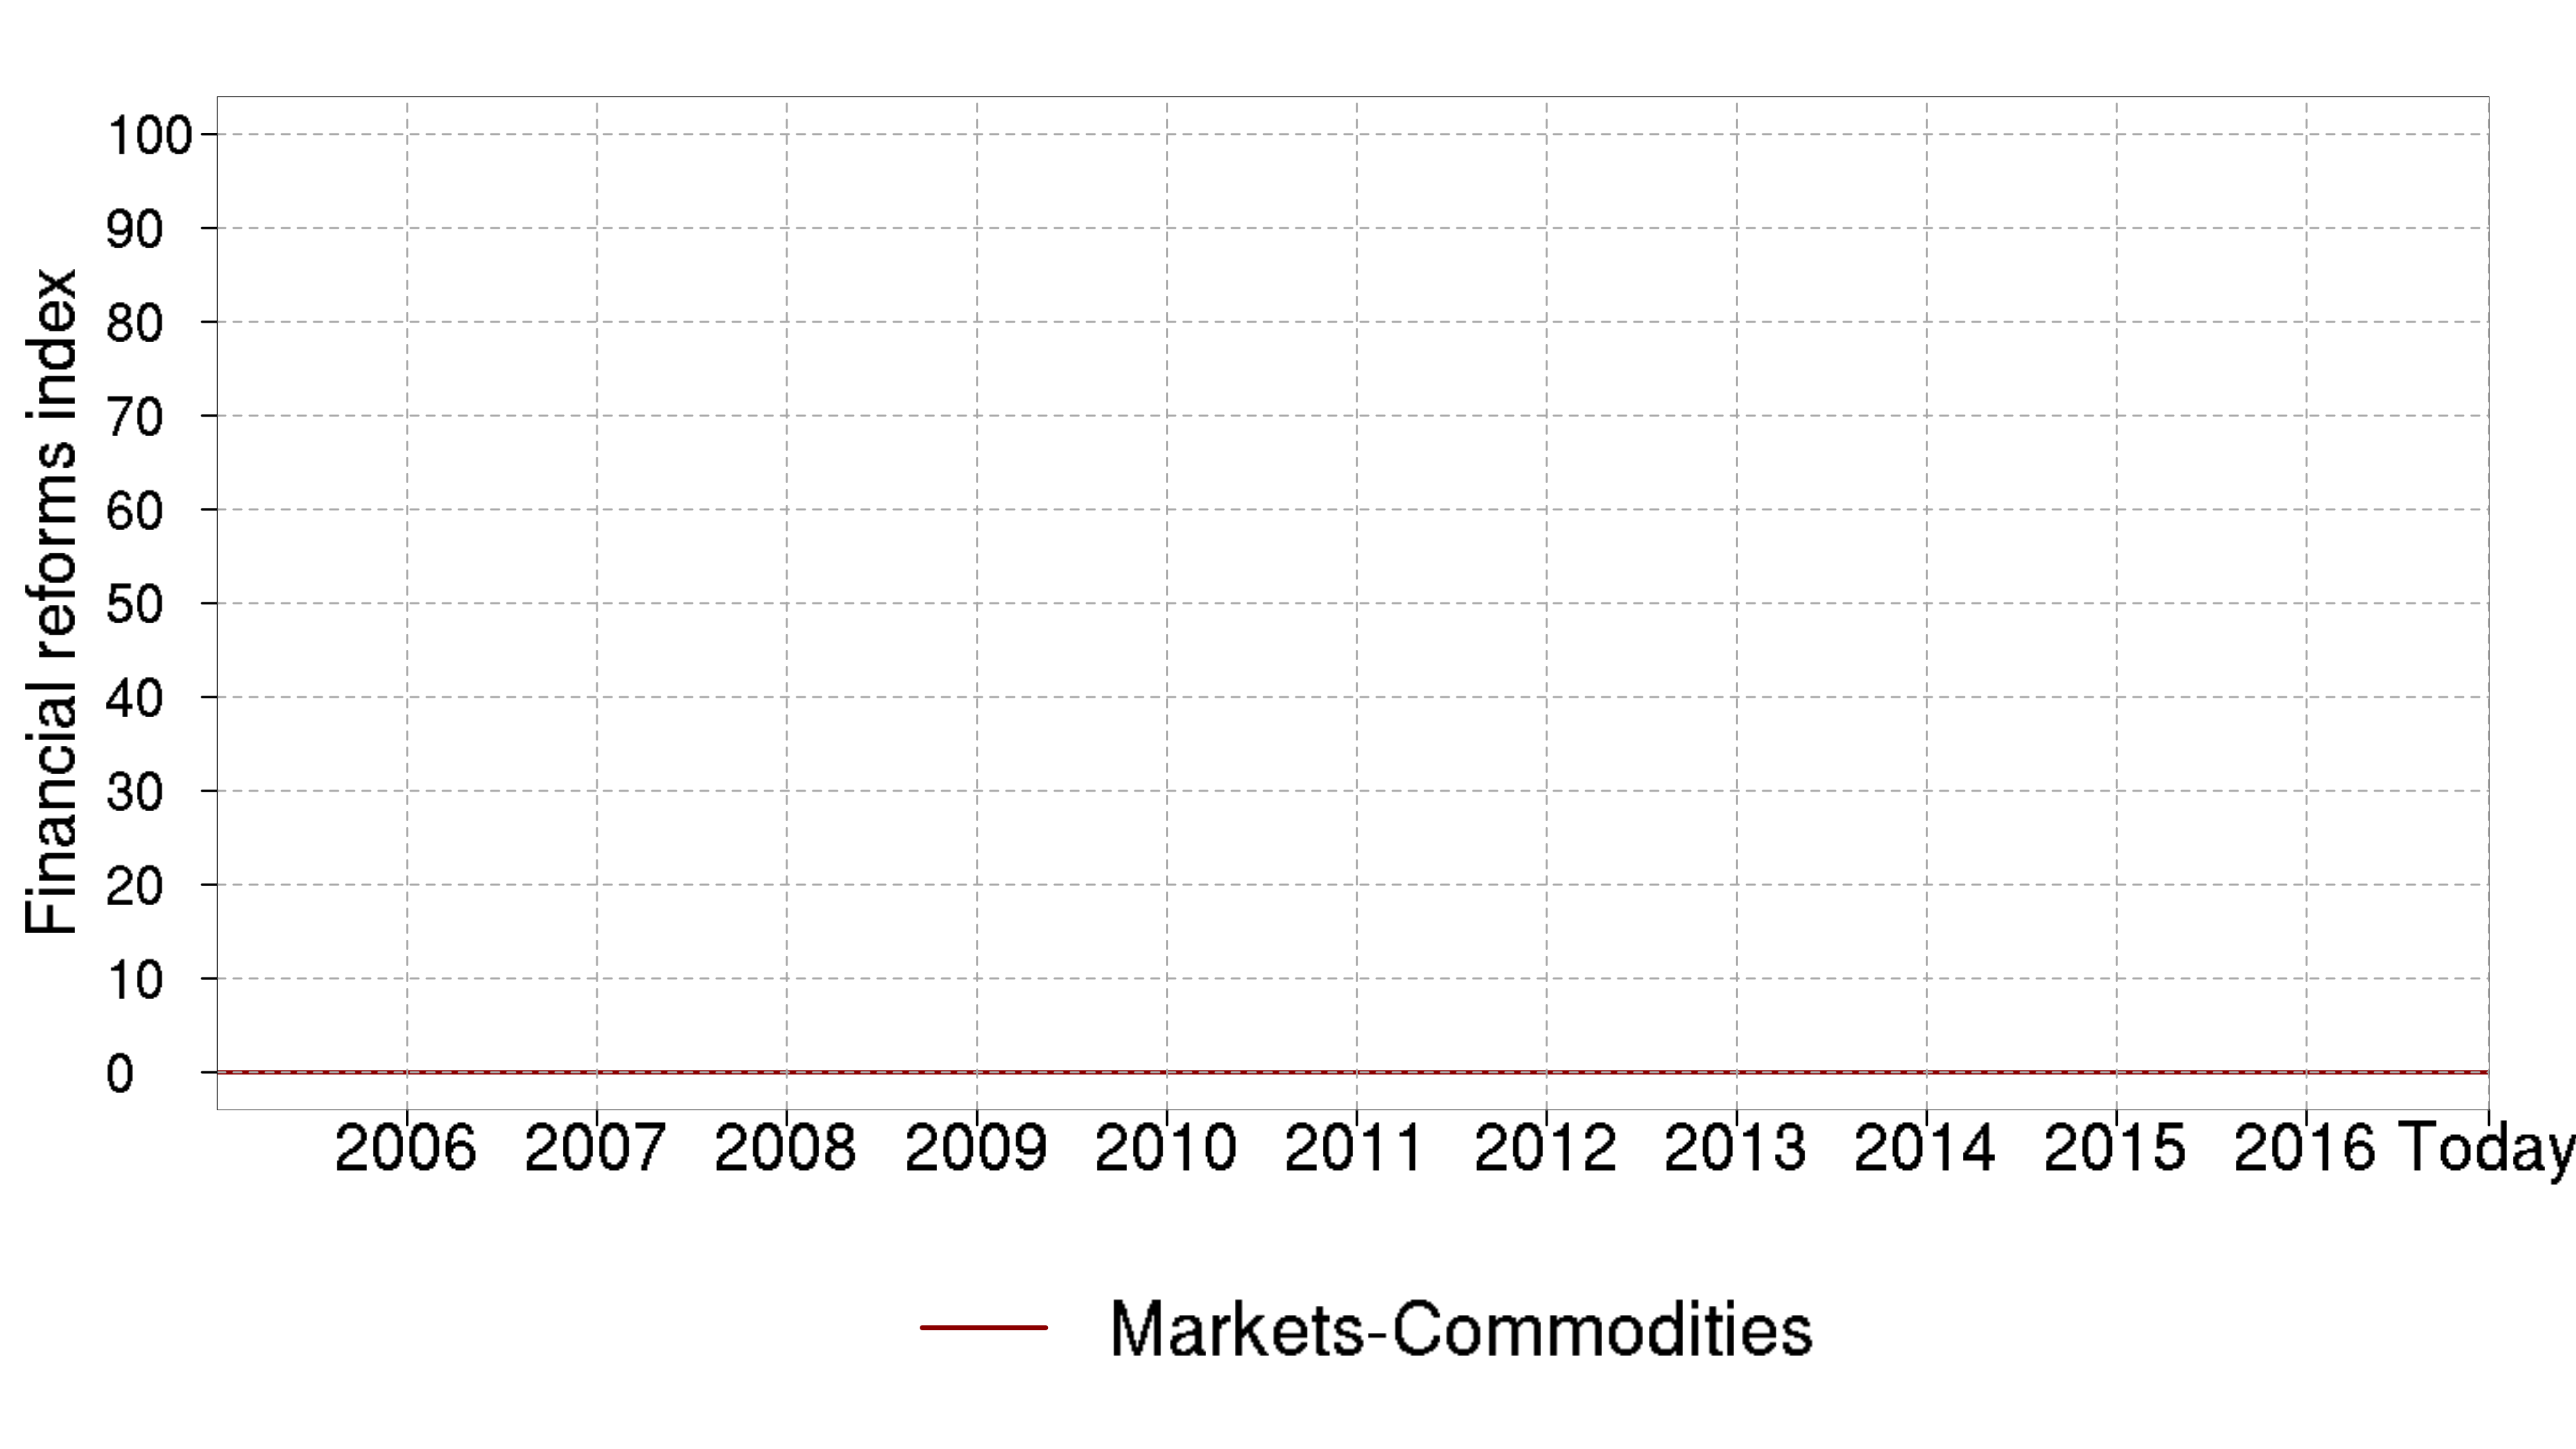
\includegraphics[width=0.65\paperwidth,height=0.45\paperwidth]{../GRAPHS/frm_index_markets_commodities.png}
\end{figure}

\begin{titlepage}
  \vspace*{\stretch{1}}

  \parbox{\textwidthorig}{
  \hrule
  \vspace{\baselineskip} \center{\Large Section index: Markets}
  \vspace{\baselineskip}
  \hrule
  }
  \vspace{\stretch{1}}

  \parbox{\textwidthorig}{
}
\end{titlepage}

\begin{table} [H]
  \caption{Section index: Markets}
  \begin{threeparttable}
    \begin{footnotesize}
      \resizebox{1\textwidth}{!}{
        \begin{tabular} {FGH}
          \multicolumn{3}{p{7in}}{\textbf{\small{Markets:}}} \\ \hline
          \textbf{Section} & \textbf{Subsection} & \textbf{Score} \\ \hline
          \input{../TABLES/frm_index_markets.tex}
          \hline
          \noalign{\vskip .01in}
          \multicolumn{3}{p{6in}}{\textit{\scriptsize{Explanation:
          Subsection-wise scores standing on \today{}.}}}
        \end{tabular}
        
      }
    \end{footnotesize}
  \end{threeparttable}
\end{table}

\begin{figure}[H]
\caption{Section index: Markets}
\centering
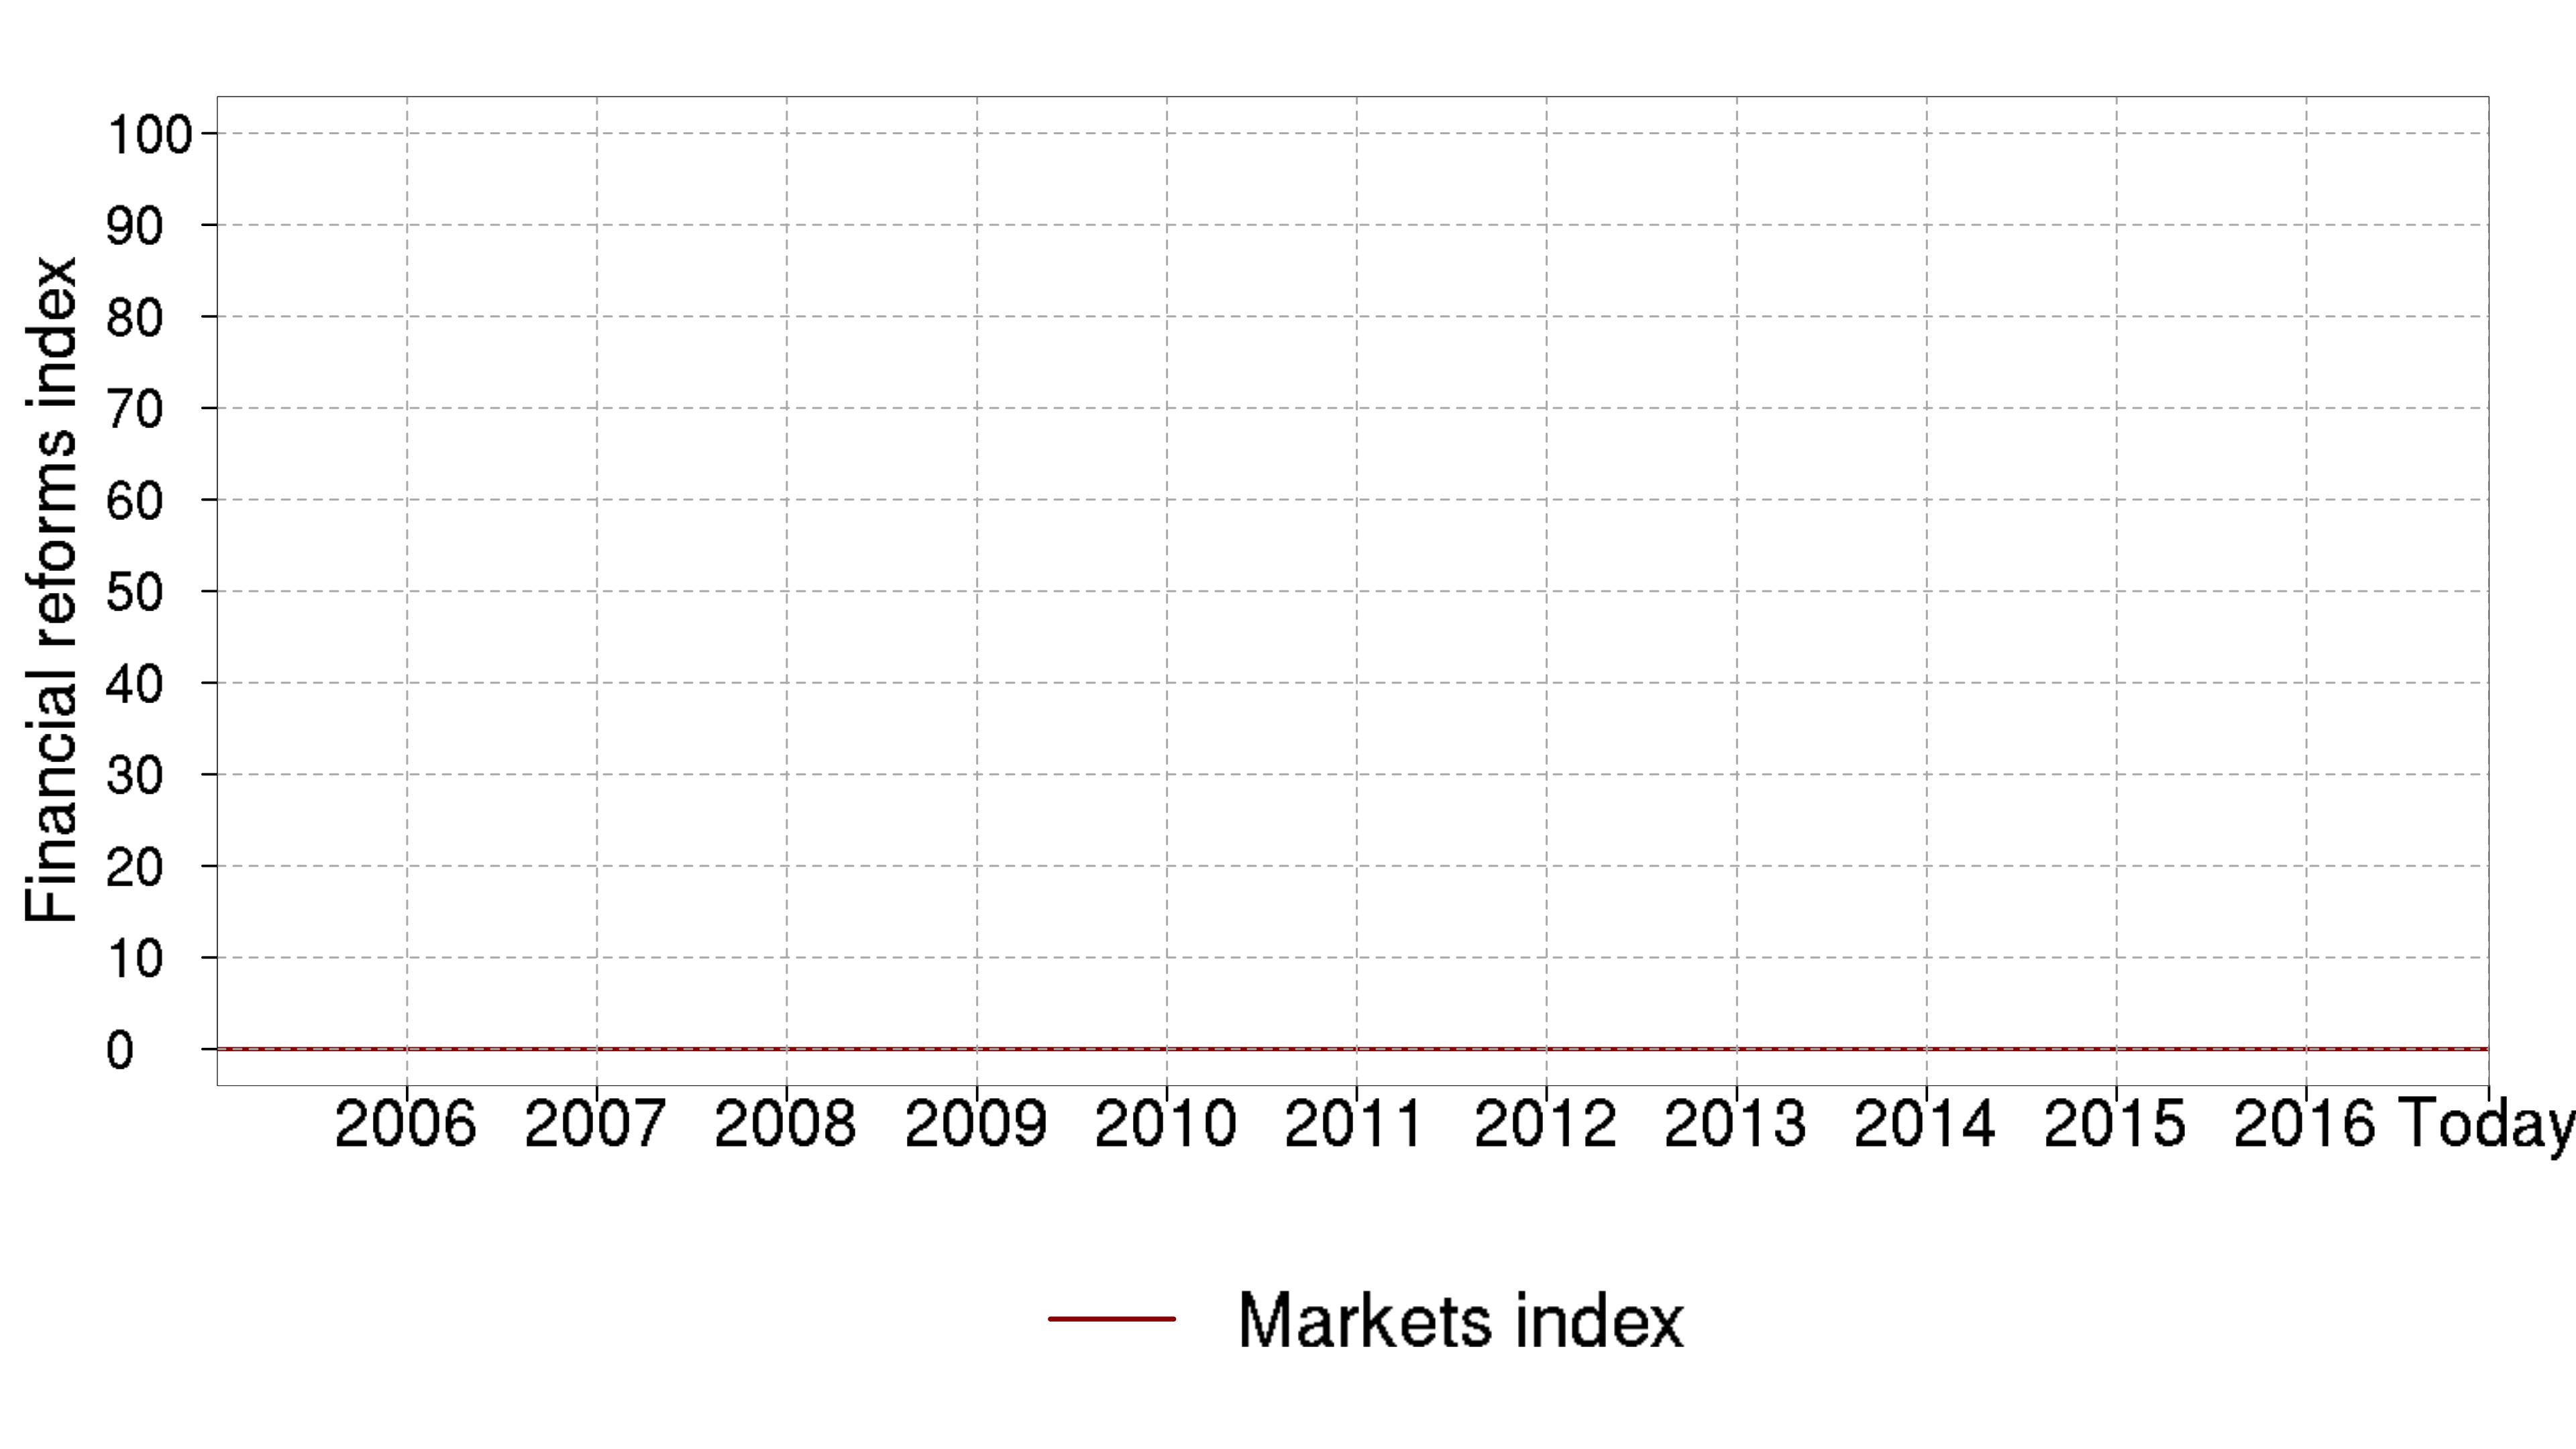
\includegraphics[width=0.9\paperwidth,height=0.7\paperwidth]{../GRAPHS/frm_index_markets.png}
\end{figure}



\begin{titlepage}
  \vspace*{\stretch{1}}

  \parbox{\textwidthorig}{
  \hrule
  \vspace{\baselineskip} \center{\Large Financial firms}
  \vspace{\baselineskip}
  \hrule
  }
  \vspace{\stretch{1}}

  \parbox{\textwidthorig}{
}

\end{titlepage}


\newpage

\refstepcounter{section}
\sectionmark{Financial firms}
\addcontentsline{toc}{section}{\protect\numberline{\thesection}Financial firms}

\begin{table} [H]
  \caption{Financial firms: Banking}
  \begin{threeparttable}
    \begin{footnotesize}
      \resizebox{1\textwidth}{!}{
        \begin{tabular} {ABCDE}
          \hline
          \noalign{\vskip .09in}
          \multicolumn{5}{p{7in}}{\textbf{\small{Financial firms:}}} \\ \hline
          \noalign{\vskip .06in}
          \multicolumn{5}{p{7in}}{\textbf{\textit{\footnotesize{Banking:}}}} \\ \hline
          \noalign{\vskip .01in}
          \multicolumn{3}{c}{\textbf{\underline{\footnotesize{Licensing, Entry barriers}}}} & \multicolumn{2}{c}{\textbf{\footnotesize{\colorbox{lightgray}{weight: 20}}}}  \\ \hline
          \noalign{\vskip .01in}
          \textbf{Date} & \textbf{Milestone} & \textbf{URL} & \textbf{Story} & \textbf{Score} \\ \hline
          \input{../TABLES/financial_firms_banking_licensingentrybarriers.tex}
          \hline
          \noalign{\vskip .06in}
          \multicolumn{3}{c}{\textbf{\underline{\footnotesize{Sound regulatory arrangement}}}} & \multicolumn{2}{c}{\textbf{\footnotesize{\colorbox{lightgray}{weight:20}}}}  \\ \hline
          \noalign{\vskip .01in}
          \textbf{Date} & \textbf{Milestone} & \textbf{URL} & \textbf{Story} & \textbf{Score} \\ \hline
          \input{../TABLES/financial_firms_banking_soundregulatoryarrangement.tex}
          \hline
          \noalign{\vskip .06in}
          \multicolumn{3}{c}{\textbf{\underline{\footnotesize{Sound regulations}}}} & \multicolumn{2}{c}{\textbf{\footnotesize{\colorbox{lightgray}{weight:20}}}}  \\ \hline
          \noalign{\vskip .01in}
          \textbf{Date} & \textbf{Milestone} & \textbf{URL} & \textbf{Story} & \textbf{Score} \\ \hline
          \input{../TABLES/financial_firms_banking_soundregulations.tex}
          \hline
          \noalign{\vskip .06in}
          \hline
          \multicolumn{3}{c}{\textbf{\underline{\footnotesize{Enforcement of regulations}}}} & \multicolumn{2}{c}{\textbf{\footnotesize{\colorbox{lightgray}{weight:20}}}}  \\ \hline
          \noalign{\vskip .01in}
          \textbf{Date} & \textbf{Milestone} & \textbf{URL} & \textbf{Story} & \textbf{Score} \\ \hline
          \input{../TABLES/financial_firms_banking_enforcementofregulations.tex}
          \hline
          \noalign{\vskip .06in}
          \hline
          \multicolumn{5}{p{6in}}{\textit{\scriptsize{Explanation:
          Financial reforms for Banking sector.}}}
        \end{tabular}
      }
    \end{footnotesize}
  \end{threeparttable}
\end{table}

\begin{figure}[H]
  \caption{Financial firms: Banking}
  \centering
  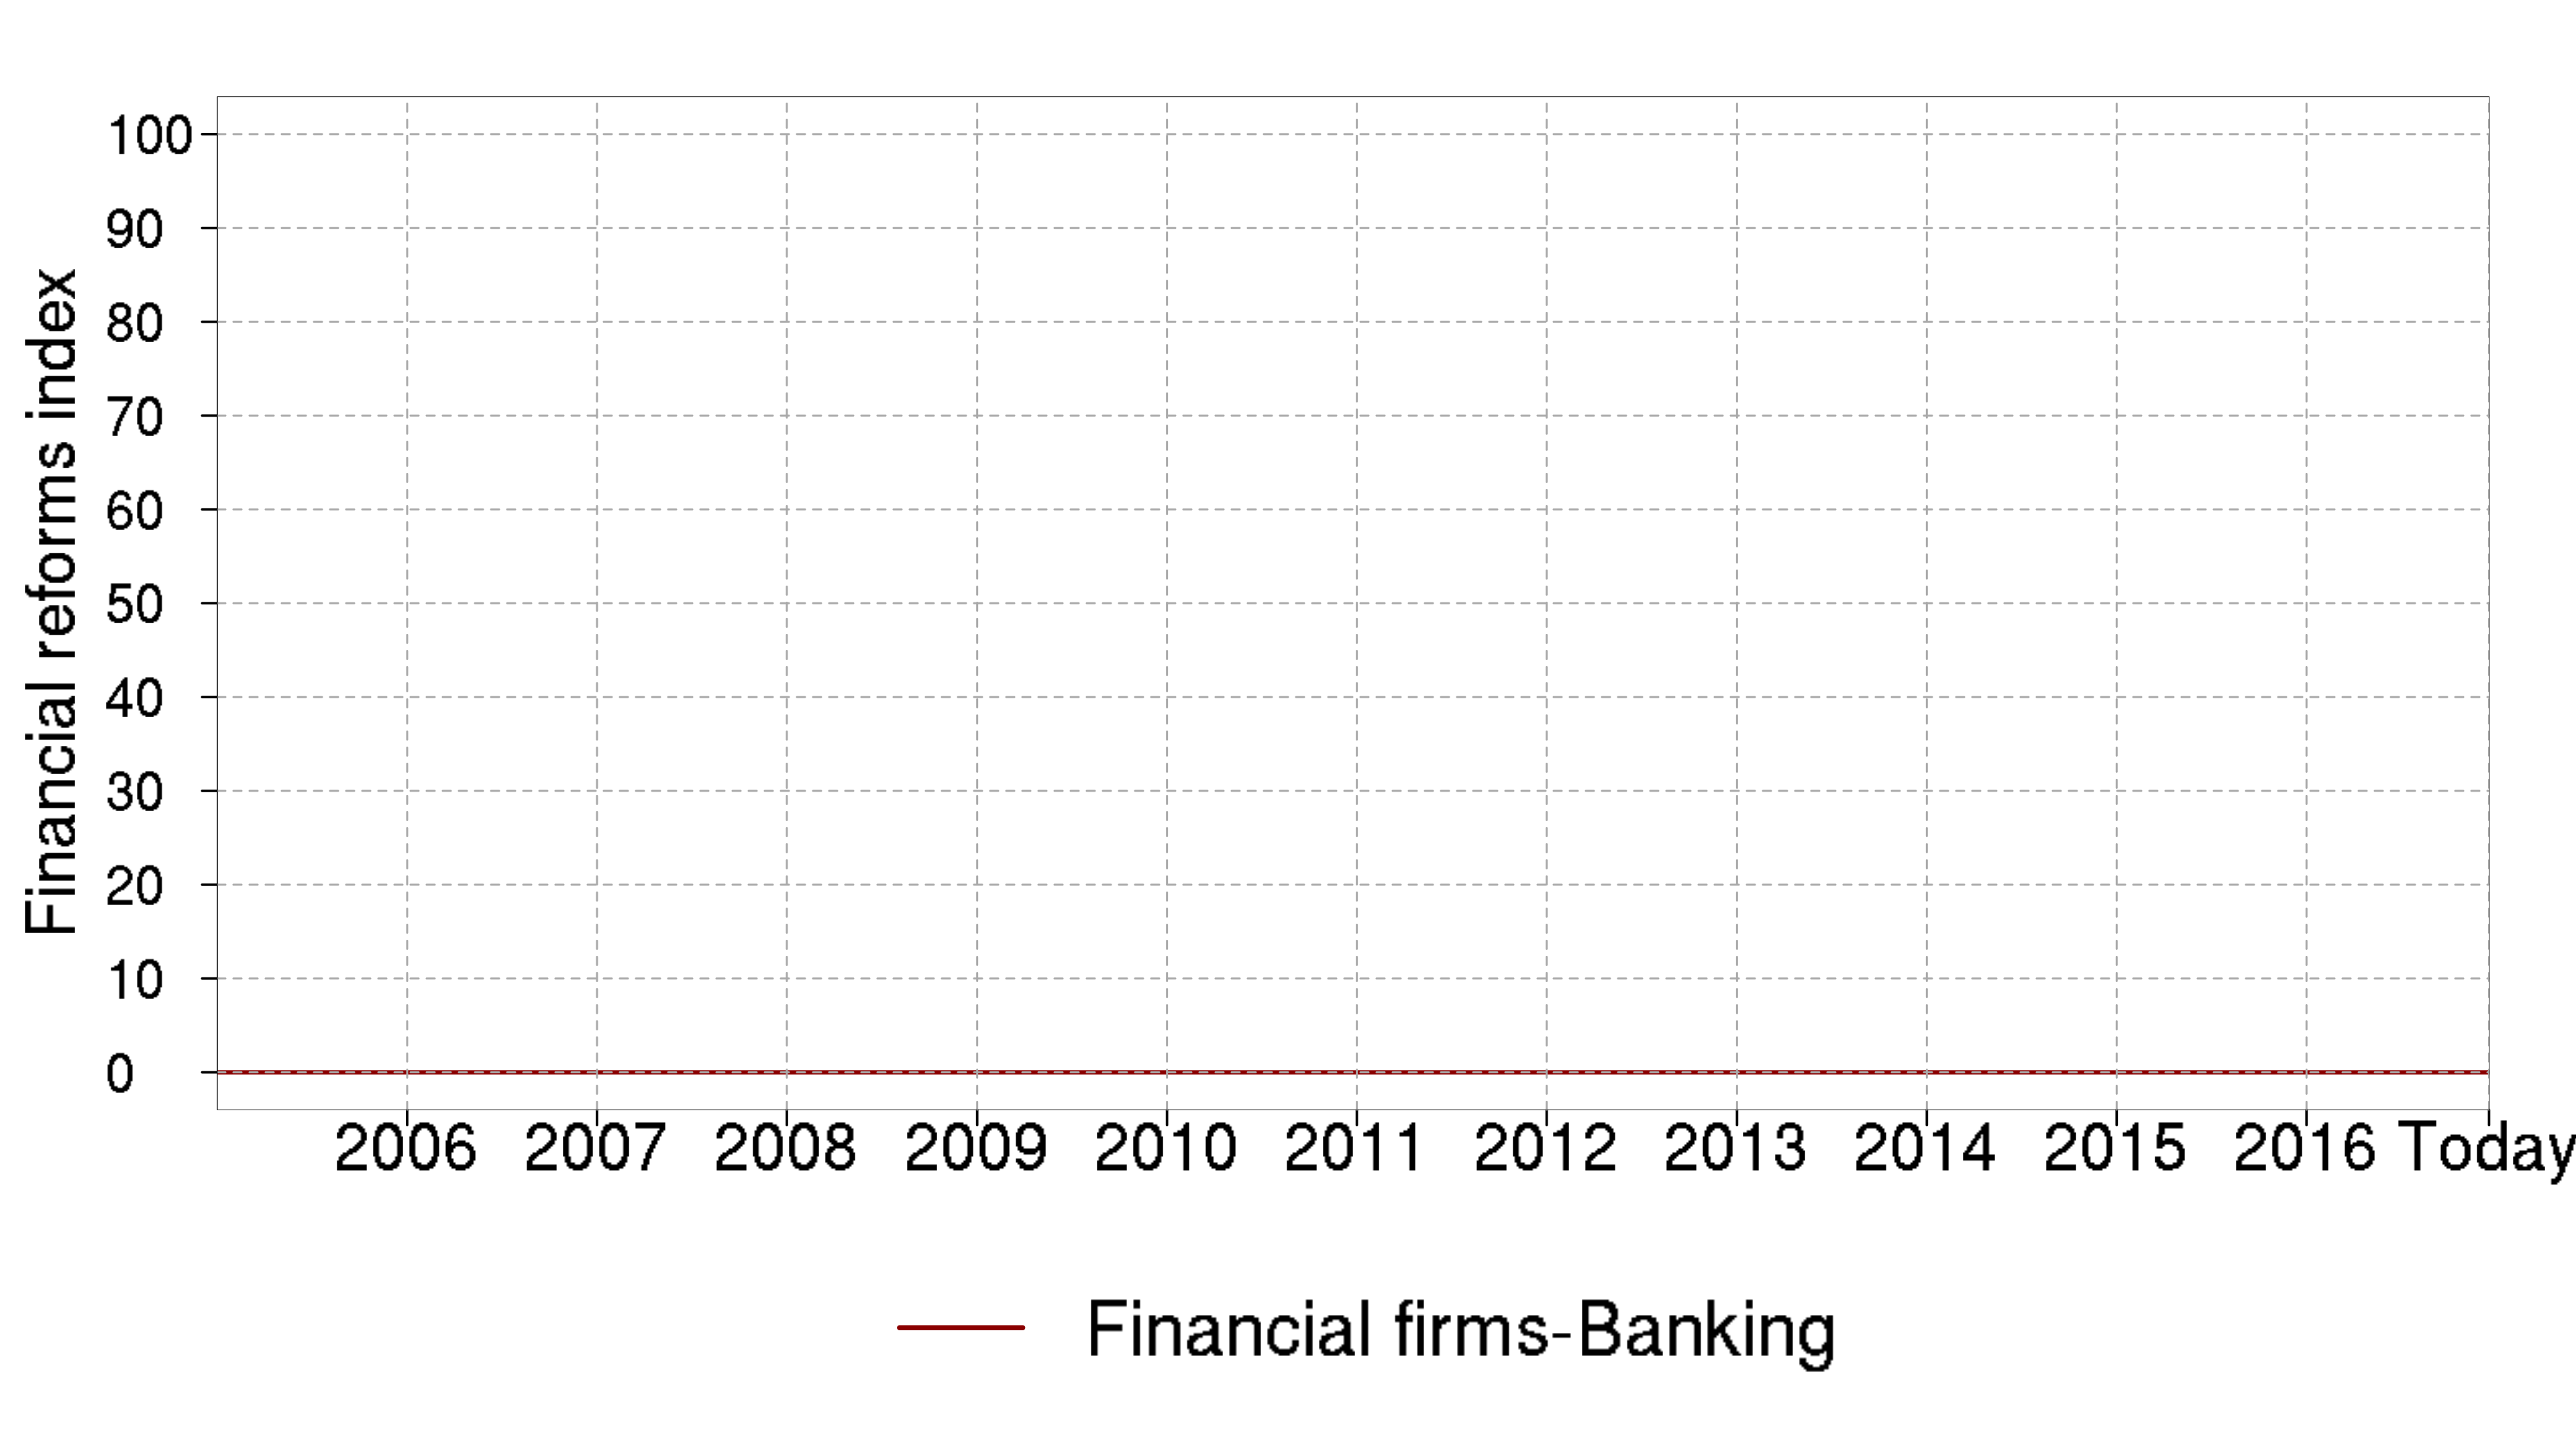
\includegraphics[width=0.65\paperwidth,height=0.45\paperwidth]{../GRAPHS/frm_index_financial_firms_banking.png}
\end{figure}

\newpage
\begin{table} [H]
  \caption{Financial firms: Payments}
  \begin{threeparttable}
    \begin{footnotesize}
      \resizebox{1\textwidth}{!}{
        \begin{tabular} {ABCDE}
          \hline
          \noalign{\vskip .09in}
          \multicolumn{5}{p{7in}}{\textbf{\small{Financial firms:}}} \\ \hline
          \noalign{\vskip .06in}
          \multicolumn{5}{p{7in}}{\textbf{\textit{\footnotesize{Payments:}}}} \\ \hline
          \noalign{\vskip .01in}
          \multicolumn{3}{c}{\textbf{\underline{\footnotesize{Licensing, Entry barriers}}}} & \multicolumn{2}{c}{\textbf{\footnotesize{\colorbox{lightgray}{weight: 20}}}}  \\ \hline
          \noalign{\vskip .01in}
          \textbf{Date} & \textbf{Milestone} & \textbf{URL} & \textbf{Story} & \textbf{Score} \\ \hline
          \input{../TABLES/financial_firms_payments_licensingentrybarriers.tex}
          \hline
          \noalign{\vskip .06in}
          \multicolumn{3}{c}{\textbf{\underline{\footnotesize{Sound regulatory arrangement}}}} & \multicolumn{2}{c}{\textbf{\footnotesize{\colorbox{lightgray}{weight:20}}}}  \\ \hline
          \noalign{\vskip .01in}
          \textbf{Date} & \textbf{Milestone} & \textbf{URL} & \textbf{Story} & \textbf{Score} \\ \hline
          \input{../TABLES/financial_firms_payments_soundregulatoryarrangement.tex}
          \hline
          \noalign{\vskip .06in}
          \multicolumn{3}{c}{\textbf{\underline{\footnotesize{Sound regulations}}}} & \multicolumn{2}{c}{\textbf{\footnotesize{\colorbox{lightgray}{weight:20}}}}  \\ \hline
          \noalign{\vskip .01in}
          \textbf{Date} & \textbf{Milestone} & \textbf{URL} & \textbf{Story} & \textbf{Score} \\ \hline
          \input{../TABLES/financial_firms_payments_soundregulations.tex}
          \hline
          \noalign{\vskip .06in}
          \hline
          \multicolumn{3}{c}{\textbf{\underline{\footnotesize{Enforcement of regulations}}}} & \multicolumn{2}{c}{\textbf{\footnotesize{\colorbox{lightgray}{weight:20}}}}  \\ \hline
          \noalign{\vskip .01in}
          \textbf{Date} & \textbf{Milestone} & \textbf{URL} & \textbf{Story} & \textbf{Score} \\ \hline
          \input{../TABLES/financial_firms_payments_enforcementofregulations.tex}
          \hline
          \noalign{\vskip .06in}
          \hline
          \multicolumn{5}{p{6in}}{\textit{\scriptsize{Explanation:
          Financial reforms for Payments sector.}}}
        \end{tabular}
      }
    \end{footnotesize}
  \end{threeparttable}
\end{table}

\begin{figure}[H]
  \caption{Financial firms: Payments}
  \centering
  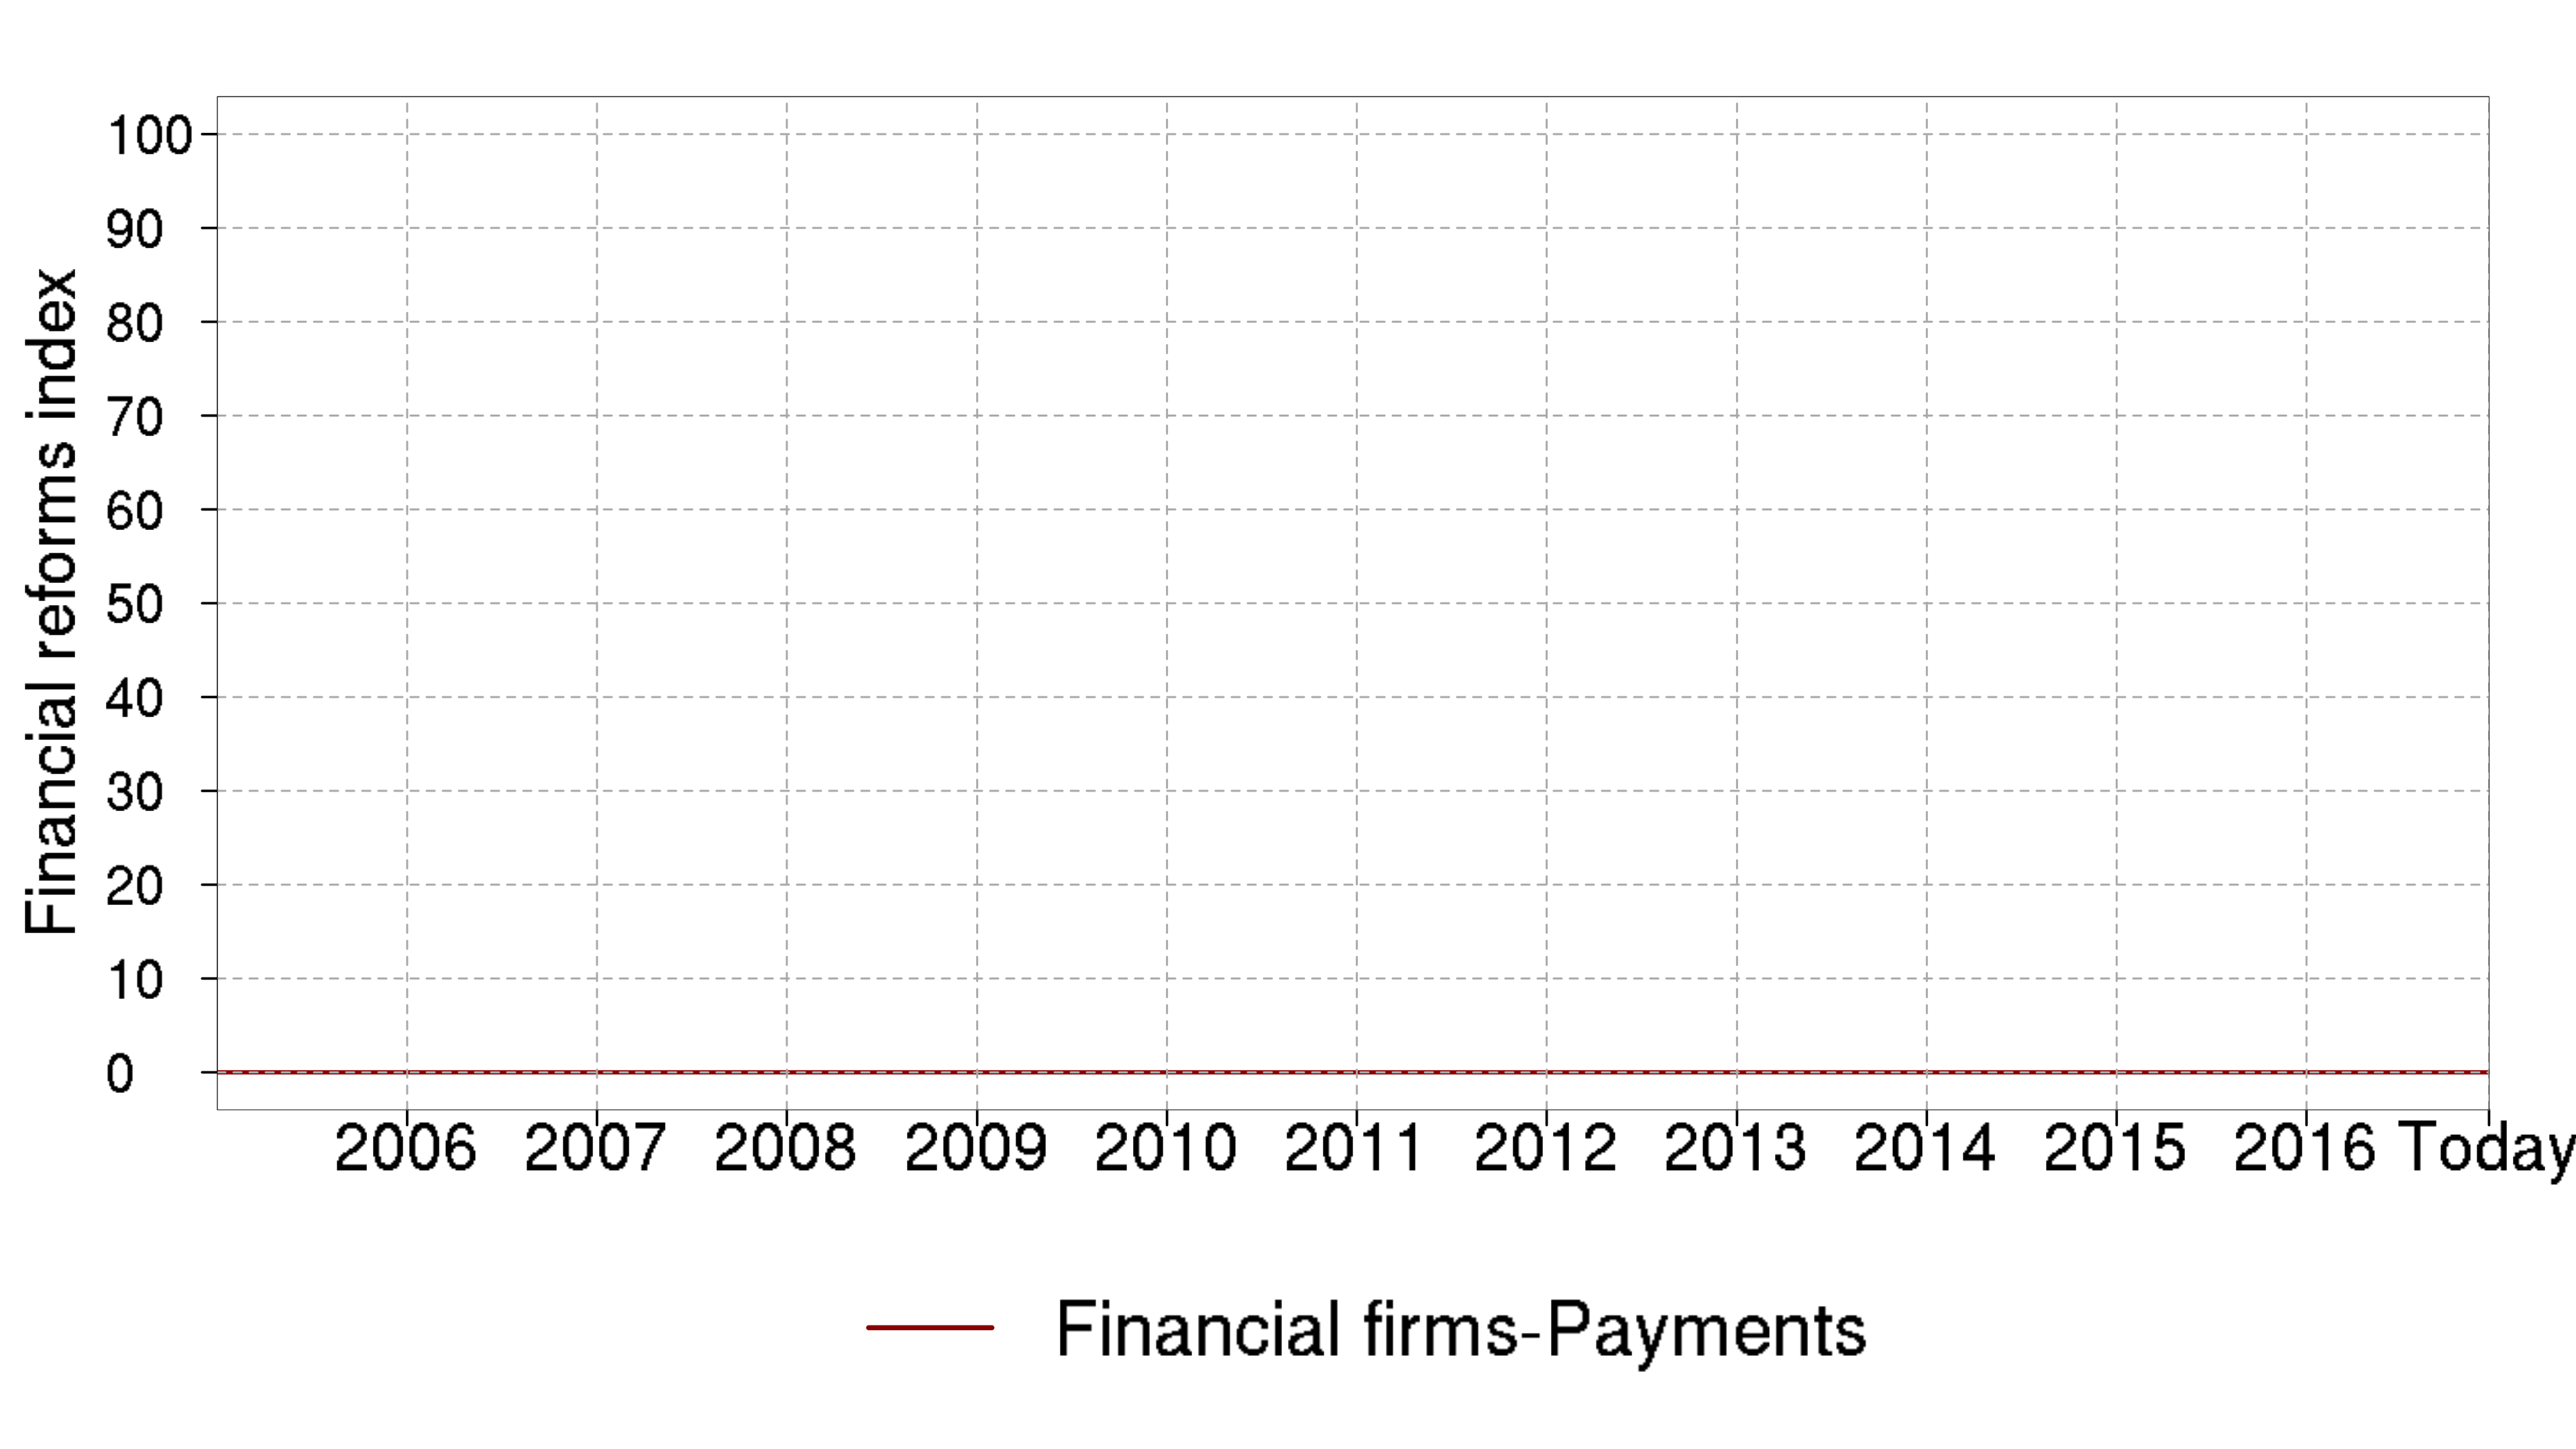
\includegraphics[width=0.65\paperwidth,height=0.45\paperwidth]{../GRAPHS/frm_index_financial_firms_payments.png}
\end{figure}

\newpage
\begin{table} [H]
  \caption{Financial firms: Insurance}
  \begin{threeparttable}
    \begin{footnotesize}
      \resizebox{1\textwidth}{!}{
        \begin{tabular} {ABCDE}
          \hline
          \noalign{\vskip .09in}
          \multicolumn{5}{p{7in}}{\textbf{\small{Financial firms:}}} \\ \hline
          \noalign{\vskip .06in}
          \multicolumn{5}{p{7in}}{\textbf{\textit{\footnotesize{Insurance:}}}} \\ \hline
          \noalign{\vskip .01in}
          \multicolumn{3}{c}{\textbf{\underline{\footnotesize{Licensing, Entry barriers}}}} & \multicolumn{2}{c}{\textbf{\footnotesize{\colorbox{lightgray}{weight: 20}}}}  \\ \hline
          \noalign{\vskip .01in}
          \textbf{Date} & \textbf{Milestone} & \textbf{URL} & \textbf{Story} & \textbf{Score} \\ \hline
          \input{../TABLES/financial_firms_insurance_licensingentrybarriers.tex}
          \hline
          \noalign{\vskip .06in}
          \multicolumn{3}{c}{\textbf{\underline{\footnotesize{Sound regulatory arrangement}}}} & \multicolumn{2}{c}{\textbf{\footnotesize{\colorbox{lightgray}{weight:20}}}}  \\ \hline
          \noalign{\vskip .01in}
          \textbf{Date} & \textbf{Milestone} & \textbf{URL} & \textbf{Story} & \textbf{Score} \\ \hline
          \input{../TABLES/financial_firms_insurance_soundregulatoryarrangement.tex}
          \hline
          \noalign{\vskip .06in}
          \multicolumn{3}{c}{\textbf{\underline{\footnotesize{Sound regulations}}}} & \multicolumn{2}{c}{\textbf{\footnotesize{\colorbox{lightgray}{weight:20}}}}  \\ \hline
          \noalign{\vskip .01in}
          \textbf{Date} & \textbf{Milestone} & \textbf{URL} & \textbf{Story} & \textbf{Score} \\ \hline
          \input{../TABLES/financial_firms_insurance_soundregulations.tex}
          \hline
          \noalign{\vskip .06in}
          \hline
          \multicolumn{3}{c}{\textbf{\underline{\footnotesize{Enforcement of regulations}}}} & \multicolumn{2}{c}{\textbf{\footnotesize{\colorbox{lightgray}{weight:20}}}}  \\ \hline
          \noalign{\vskip .01in}
          \textbf{Date} & \textbf{Milestone} & \textbf{URL} & \textbf{Story} & \textbf{Score} \\ \hline
          \input{../TABLES/financial_firms_insurance_enforcementofregulations.tex}
          \hline
          \noalign{\vskip .06in}
          \hline
          \multicolumn{5}{p{6in}}{\textit{\scriptsize{Explanation:
          Financial reforms for Insurance sector.}}}
        \end{tabular}
      }
    \end{footnotesize}
  \end{threeparttable}
\end{table}

\begin{figure}[H]
  \caption{Financial firms: Insurance}
  \centering
  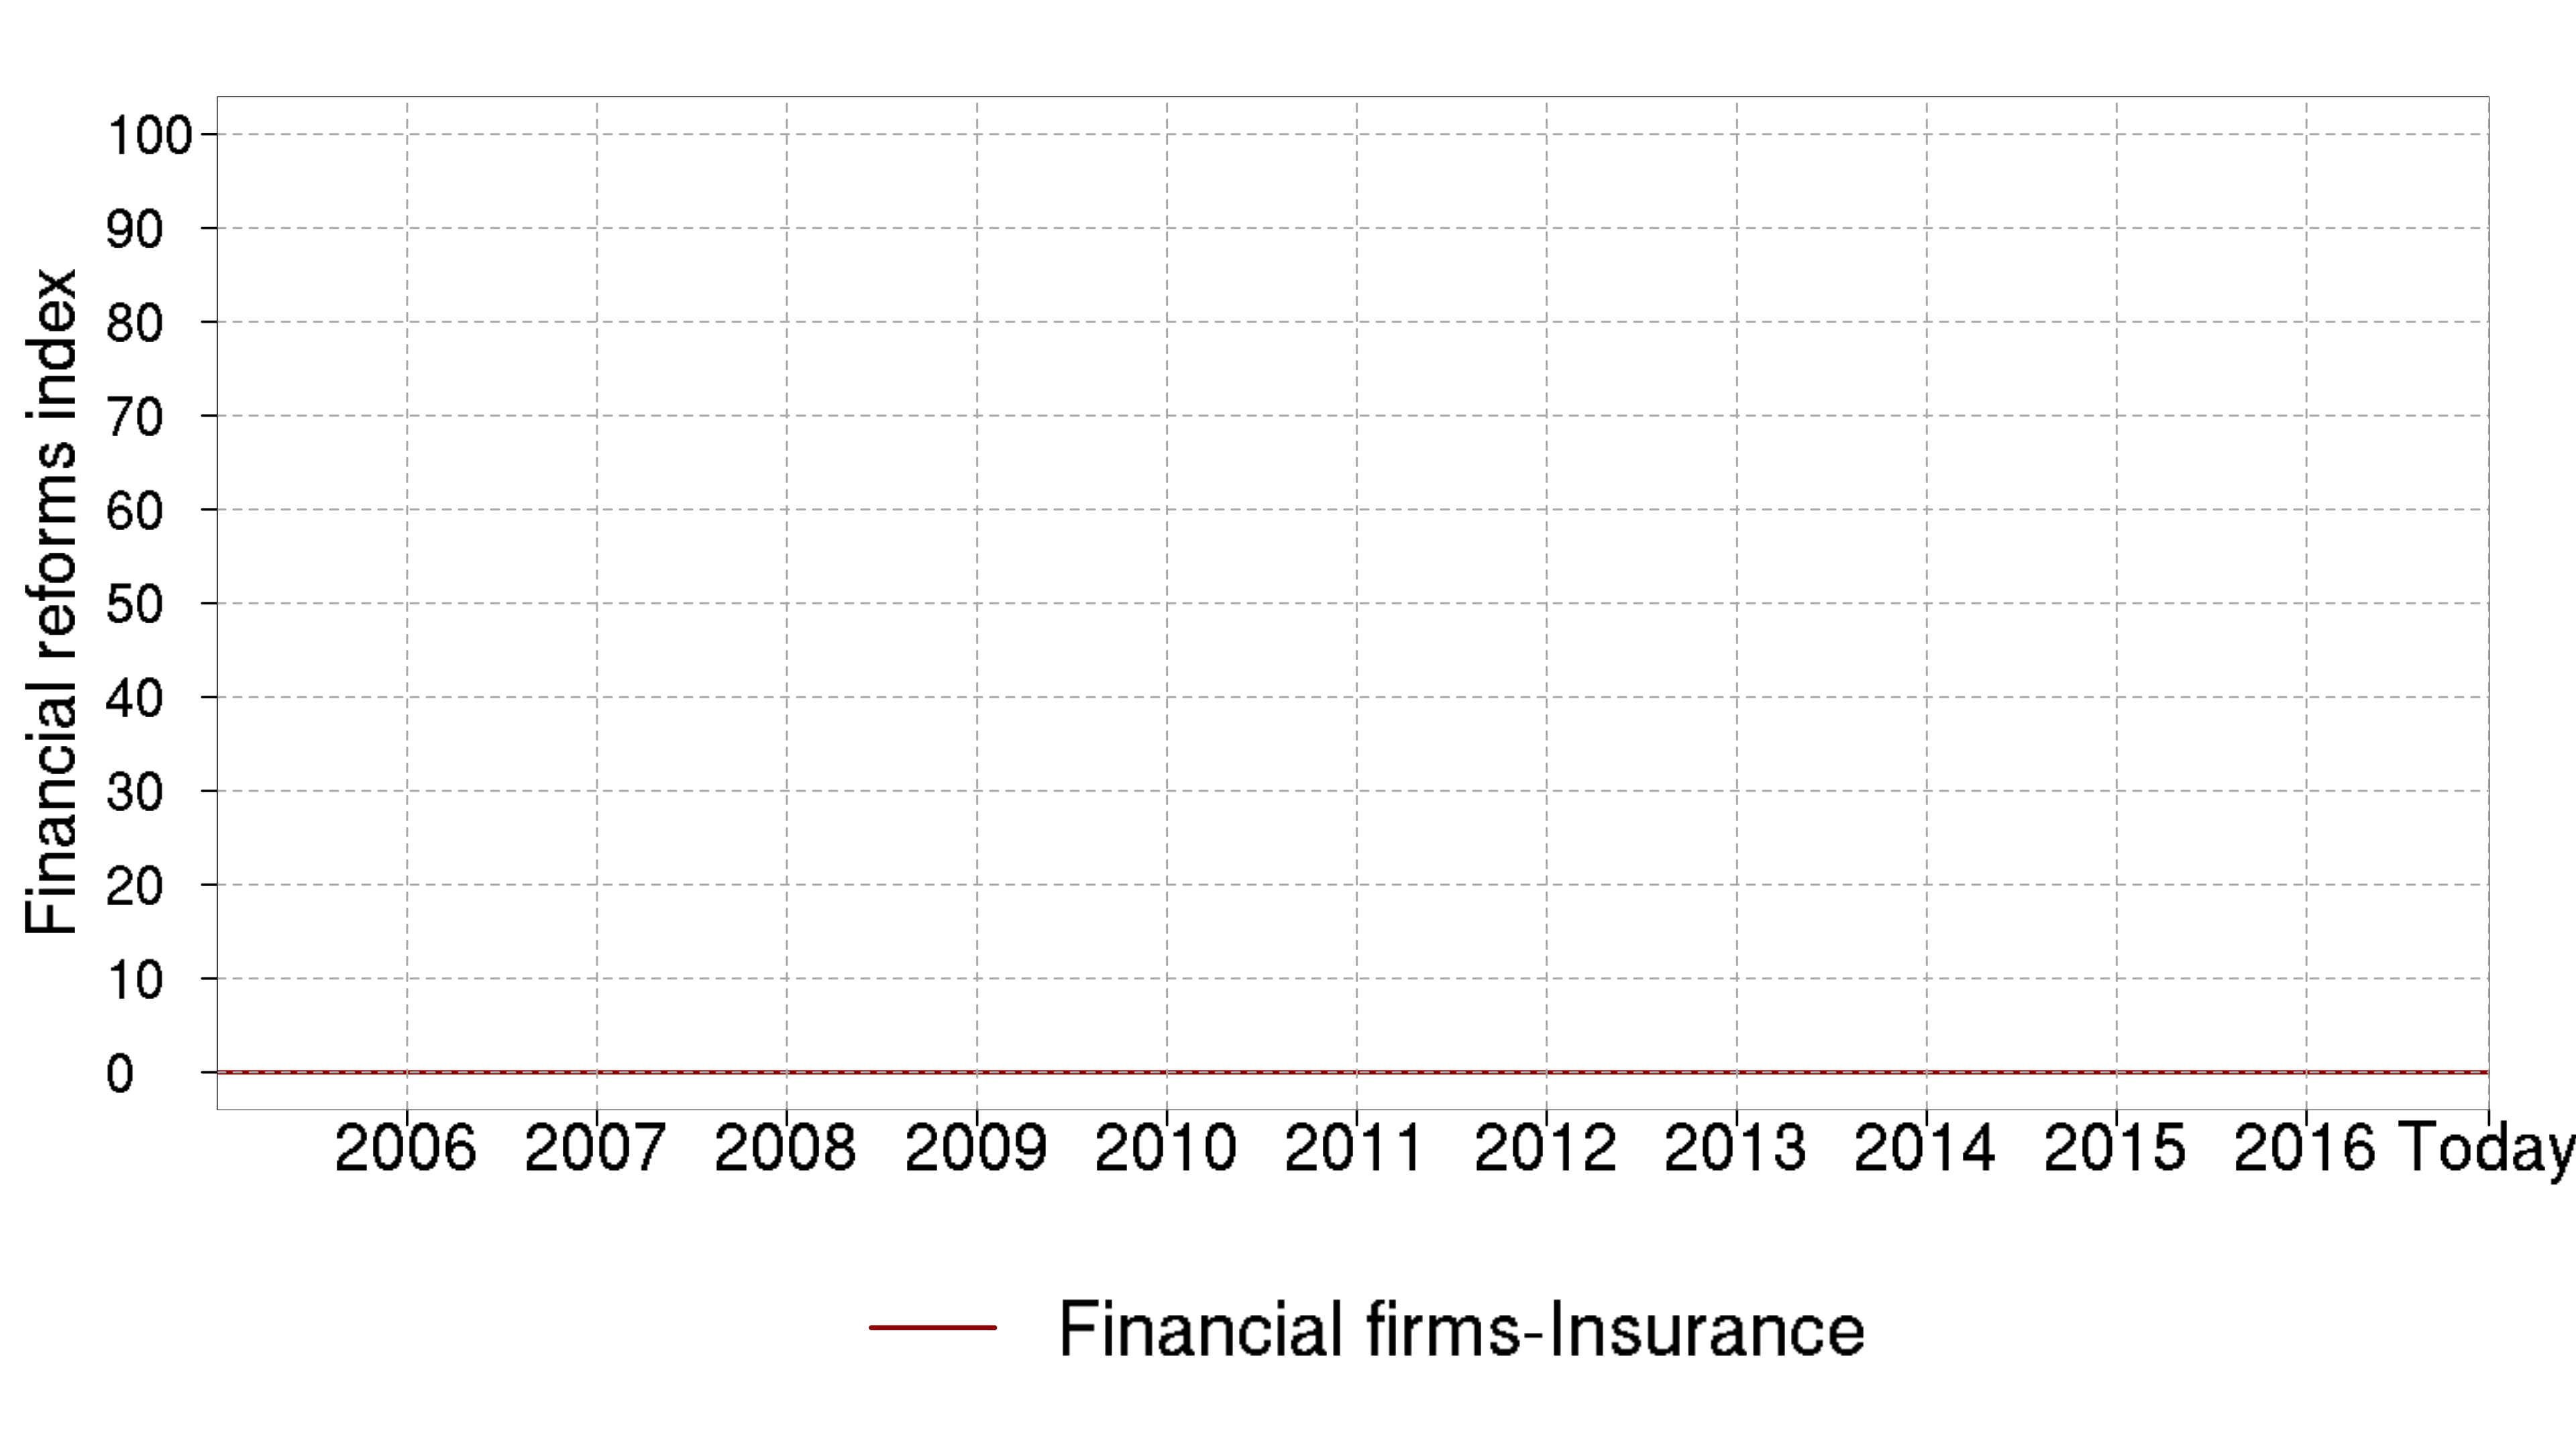
\includegraphics[width=0.65\paperwidth,height=0.45\paperwidth]{../GRAPHS/frm_index_financial_firms_insurance.png}
\end{figure}


\newpage
\begin{table} [H]
  \caption{Financial firms: Mutual funds}
  \begin{threeparttable}
    \begin{footnotesize}
      \resizebox{1\textwidth}{!}{
        \begin{tabular} {ABCDE}
          \hline
          \noalign{\vskip .09in}
          \multicolumn{5}{p{7in}}{\textbf{\small{Financial firms:}}} \\ \hline
          \noalign{\vskip .06in}
          \multicolumn{5}{p{7in}}{\textbf{\textit{\footnotesize{Mutual funds:}}}} \\ \hline
          \noalign{\vskip .01in}
          \multicolumn{3}{c}{\textbf{\underline{\footnotesize{Licensing, Entry barriers}}}} & \multicolumn{2}{c}{\textbf{\footnotesize{\colorbox{lightgray}{weight: 20}}}}  \\ \hline
          \noalign{\vskip .01in}
          \textbf{Date} & \textbf{Milestone} & \textbf{URL} & \textbf{Story} & \textbf{Score} \\ \hline
          \input{../TABLES/financial_firms_mutual_funds_licensingentrybarriers.tex}
          \hline
          \noalign{\vskip .06in}
          \multicolumn{3}{c}{\textbf{\underline{\footnotesize{Sound regulatory arrangement}}}} & \multicolumn{2}{c}{\textbf{\footnotesize{\colorbox{lightgray}{weight:20}}}}  \\ \hline
          \noalign{\vskip .01in}
          \textbf{Date} & \textbf{Milestone} & \textbf{URL} & \textbf{Story} & \textbf{Score} \\ \hline
          \input{../TABLES/financial_firms_mutual_funds_soundregulatoryarrangement.tex}
          \hline
          \noalign{\vskip .06in}
          \multicolumn{3}{c}{\textbf{\underline{\footnotesize{Sound regulations}}}} & \multicolumn{2}{c}{\textbf{\footnotesize{\colorbox{lightgray}{weight:20}}}}  \\ \hline
          \noalign{\vskip .01in}
          \textbf{Date} & \textbf{Milestone} & \textbf{URL} & \textbf{Story} & \textbf{Score} \\ \hline
          \input{../TABLES/financial_firms_mutual_funds_soundregulations.tex}
          \hline
          \noalign{\vskip .06in}
          \hline
          \multicolumn{3}{c}{\textbf{\underline{\footnotesize{Enforcement of regulations}}}} & \multicolumn{2}{c}{\textbf{\footnotesize{\colorbox{lightgray}{weight:20}}}}  \\ \hline
          \noalign{\vskip .01in}
          \textbf{Date} & \textbf{Milestone} & \textbf{URL} & \textbf{Story} & \textbf{Score} \\ \hline
          \input{../TABLES/financial_firms_mutual_funds_enforcementofregulations.tex}
          \hline
          \noalign{\vskip .06in}
          \hline
          \multicolumn{5}{p{6in}}{\textit{\scriptsize{Explanation:
          Financial reforms for Mutual funds sector.}}}
        \end{tabular}
      }
    \end{footnotesize}
  \end{threeparttable}
\end{table}

\begin{figure}[H]
  \caption{Financial firms: Mutual funds}
  \centering
  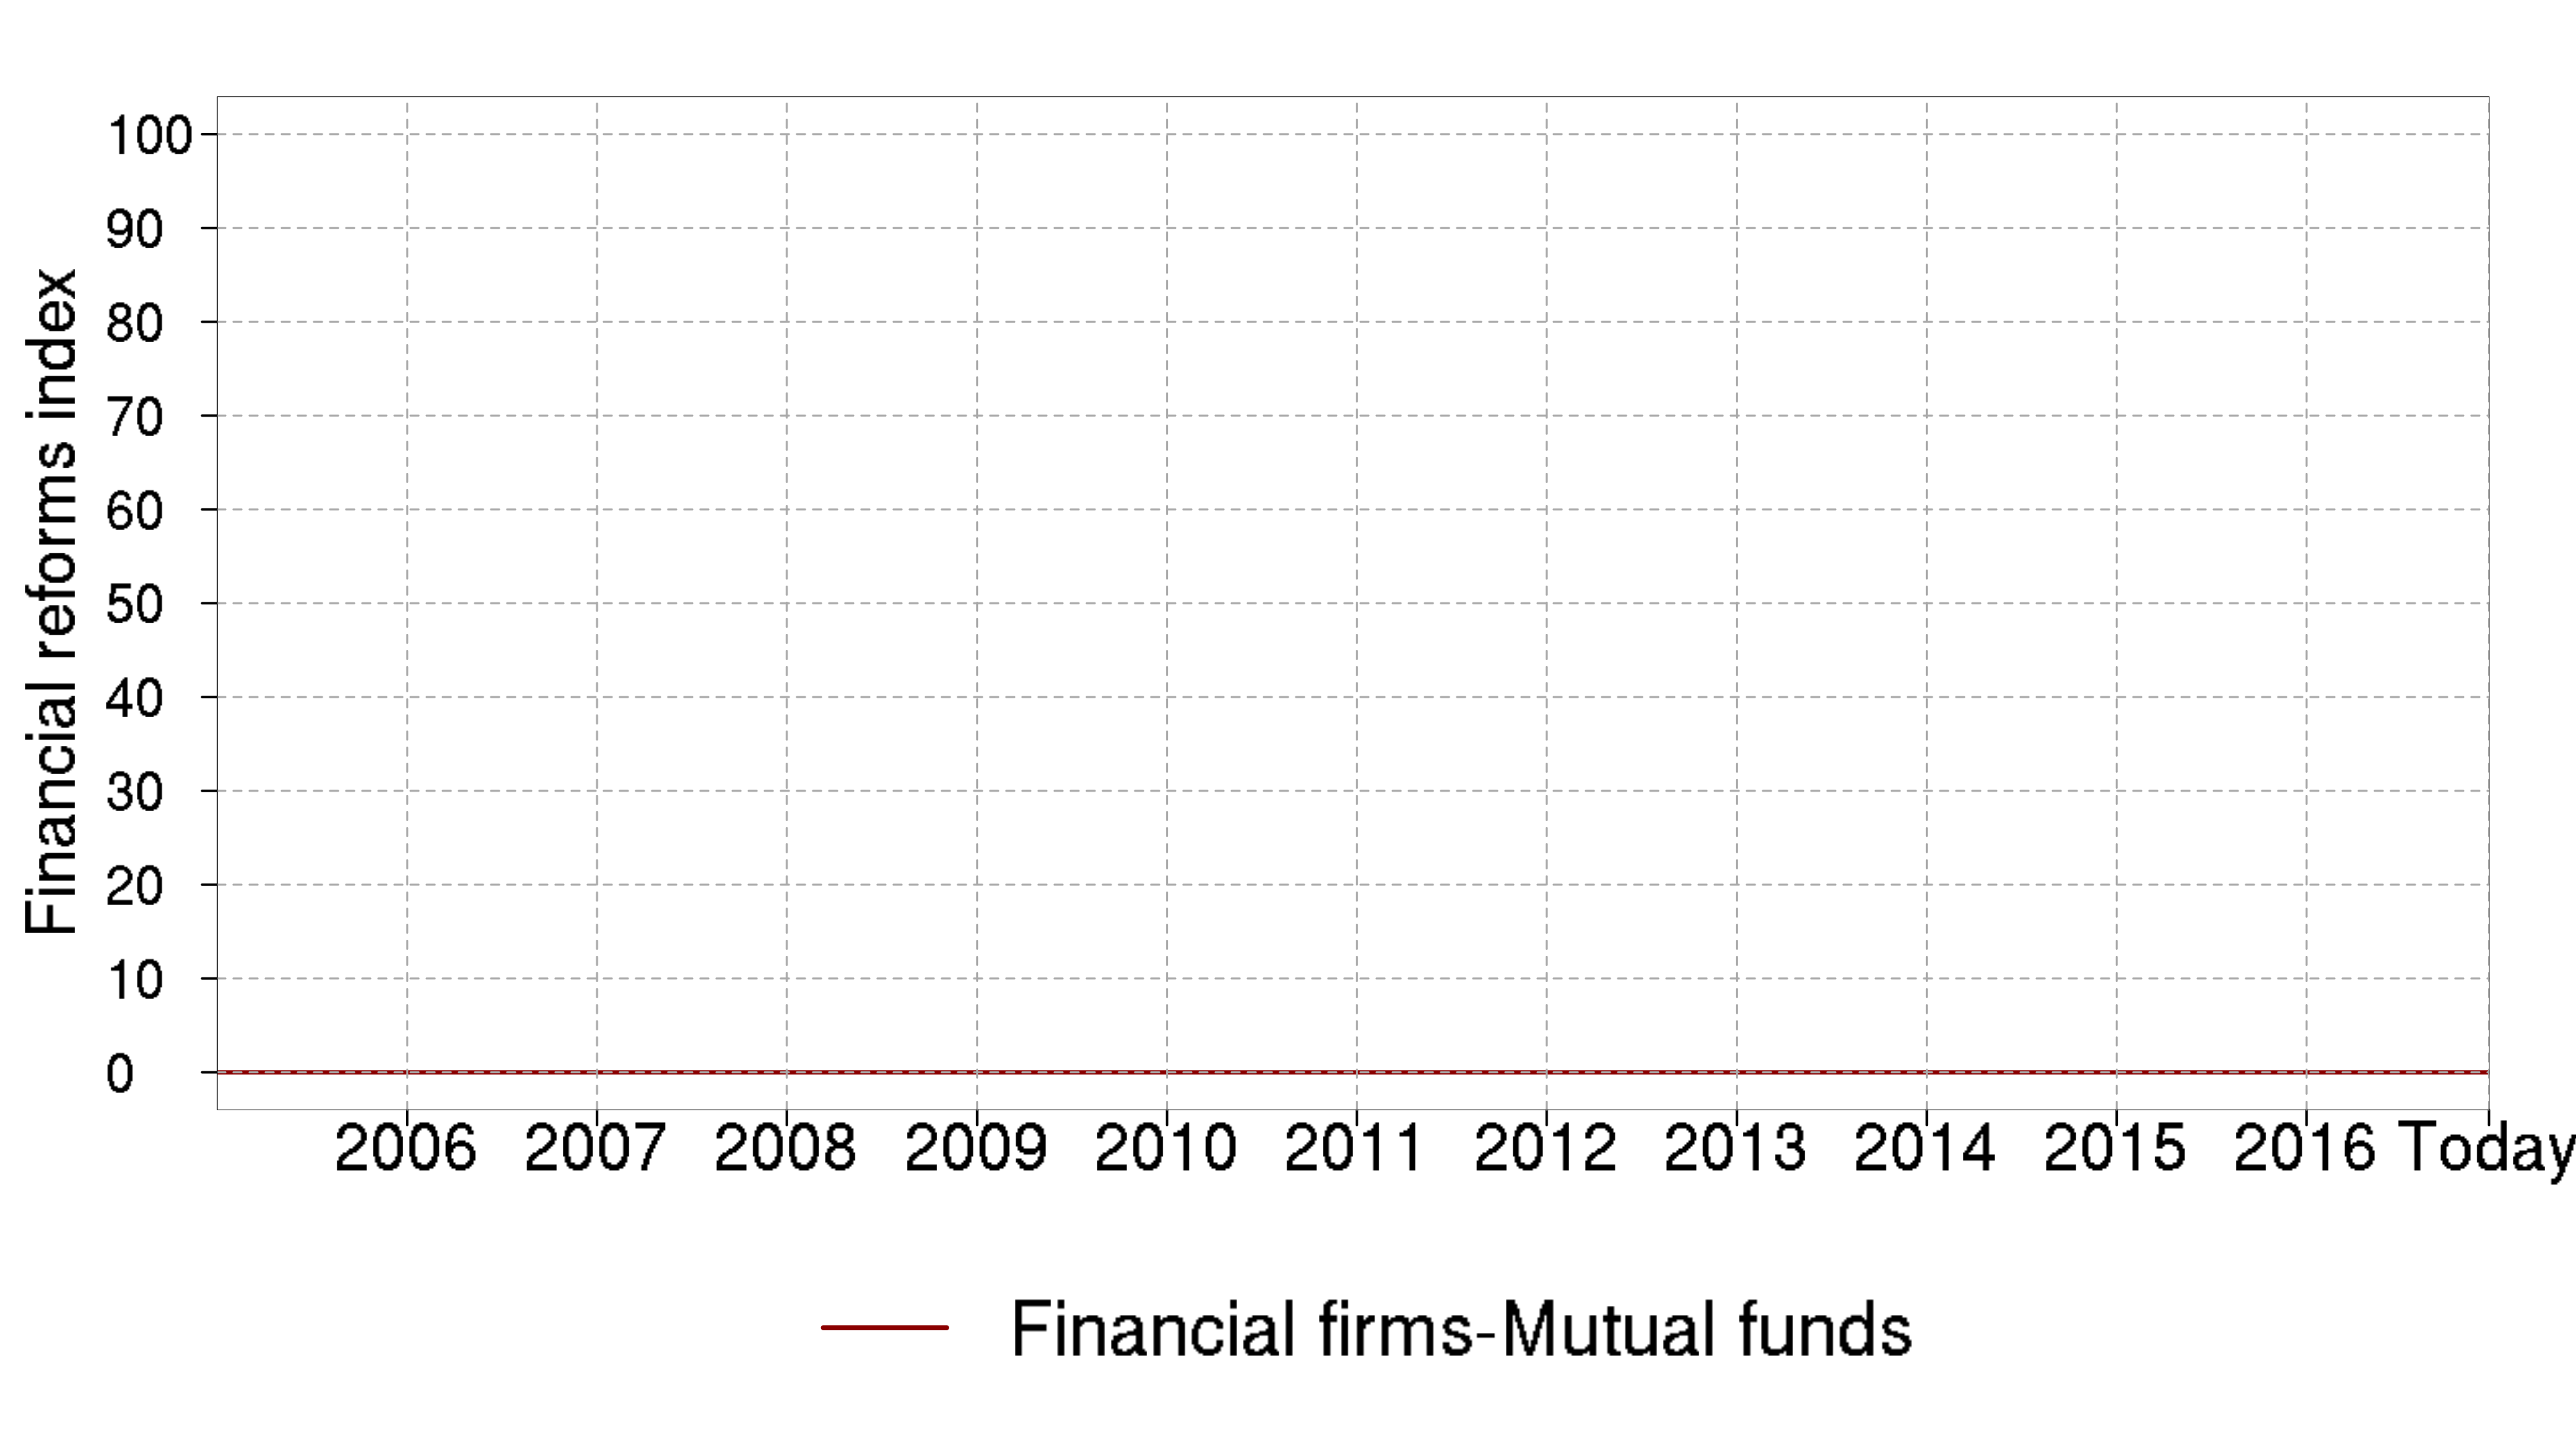
\includegraphics[width=0.65\paperwidth,height=0.45\paperwidth]{../GRAPHS/frm_index_financial_firms_mutual_funds.png}
\end{figure}


\newpage
\begin{table} [H]
  \caption{Financial firms: Pension funds}
  \begin{threeparttable}
    \begin{footnotesize}
      \resizebox{1\textwidth}{!}{
        \begin{tabular} {ABCDE}
          \hline
          \noalign{\vskip .09in}
          \multicolumn{5}{p{7in}}{\textbf{\small{Financial firms:}}} \\ \hline
          \noalign{\vskip .06in}
          \multicolumn{5}{p{7in}}{\textbf{\textit{\footnotesize{Pension funds:}}}} \\ \hline
          \noalign{\vskip .01in}
          \multicolumn{3}{c}{\textbf{\underline{\footnotesize{Licensing, Entry barriers}}}} & \multicolumn{2}{c}{\textbf{\footnotesize{\colorbox{lightgray}{weight: 20}}}}  \\ \hline
          \noalign{\vskip .01in}
          \textbf{Date} & \textbf{Milestone} & \textbf{URL} & \textbf{Story} & \textbf{Score} \\ \hline
          \input{../TABLES/financial_firms_pension_funds_licensingentrybarriers.tex}
          \hline
          \noalign{\vskip .06in}
          \multicolumn{3}{c}{\textbf{\underline{\footnotesize{Sound regulatory arrangement}}}} & \multicolumn{2}{c}{\textbf{\footnotesize{\colorbox{lightgray}{weight:20}}}}  \\ \hline
          \noalign{\vskip .01in}
          \textbf{Date} & \textbf{Milestone} & \textbf{URL} & \textbf{Story} & \textbf{Score} \\ \hline
          \input{../TABLES/financial_firms_pension_funds_soundregulatoryarrangement.tex}
          \hline
          \noalign{\vskip .06in}
          \multicolumn{3}{c}{\textbf{\underline{\footnotesize{Sound regulations}}}} & \multicolumn{2}{c}{\textbf{\footnotesize{\colorbox{lightgray}{weight:20}}}}  \\ \hline
          \noalign{\vskip .01in}
          \textbf{Date} & \textbf{Milestone} & \textbf{URL} & \textbf{Story} & \textbf{Score} \\ \hline
          \input{../TABLES/financial_firms_pension_funds_soundregulations.tex}
          \hline
          \noalign{\vskip .06in}
          \hline
          \multicolumn{3}{c}{\textbf{\underline{\footnotesize{Enforcement of regulations}}}} & \multicolumn{2}{c}{\textbf{\footnotesize{\colorbox{lightgray}{weight:20}}}}  \\ \hline
          \noalign{\vskip .01in}
          \textbf{Date} & \textbf{Milestone} & \textbf{URL} & \textbf{Story} & \textbf{Score} \\ \hline
          \input{../TABLES/financial_firms_pension_funds_enforcementofregulations.tex}
          \hline
          \noalign{\vskip .06in}
          \hline
          \multicolumn{5}{p{6in}}{\textit{\scriptsize{Explanation:
          Financial reforms for Pension funds sector.}}}
        \end{tabular}
      }
    \end{footnotesize}
  \end{threeparttable}
\end{table}

\begin{figure}[H]
  \caption{Financial firms: Pension funds}
  \centering
  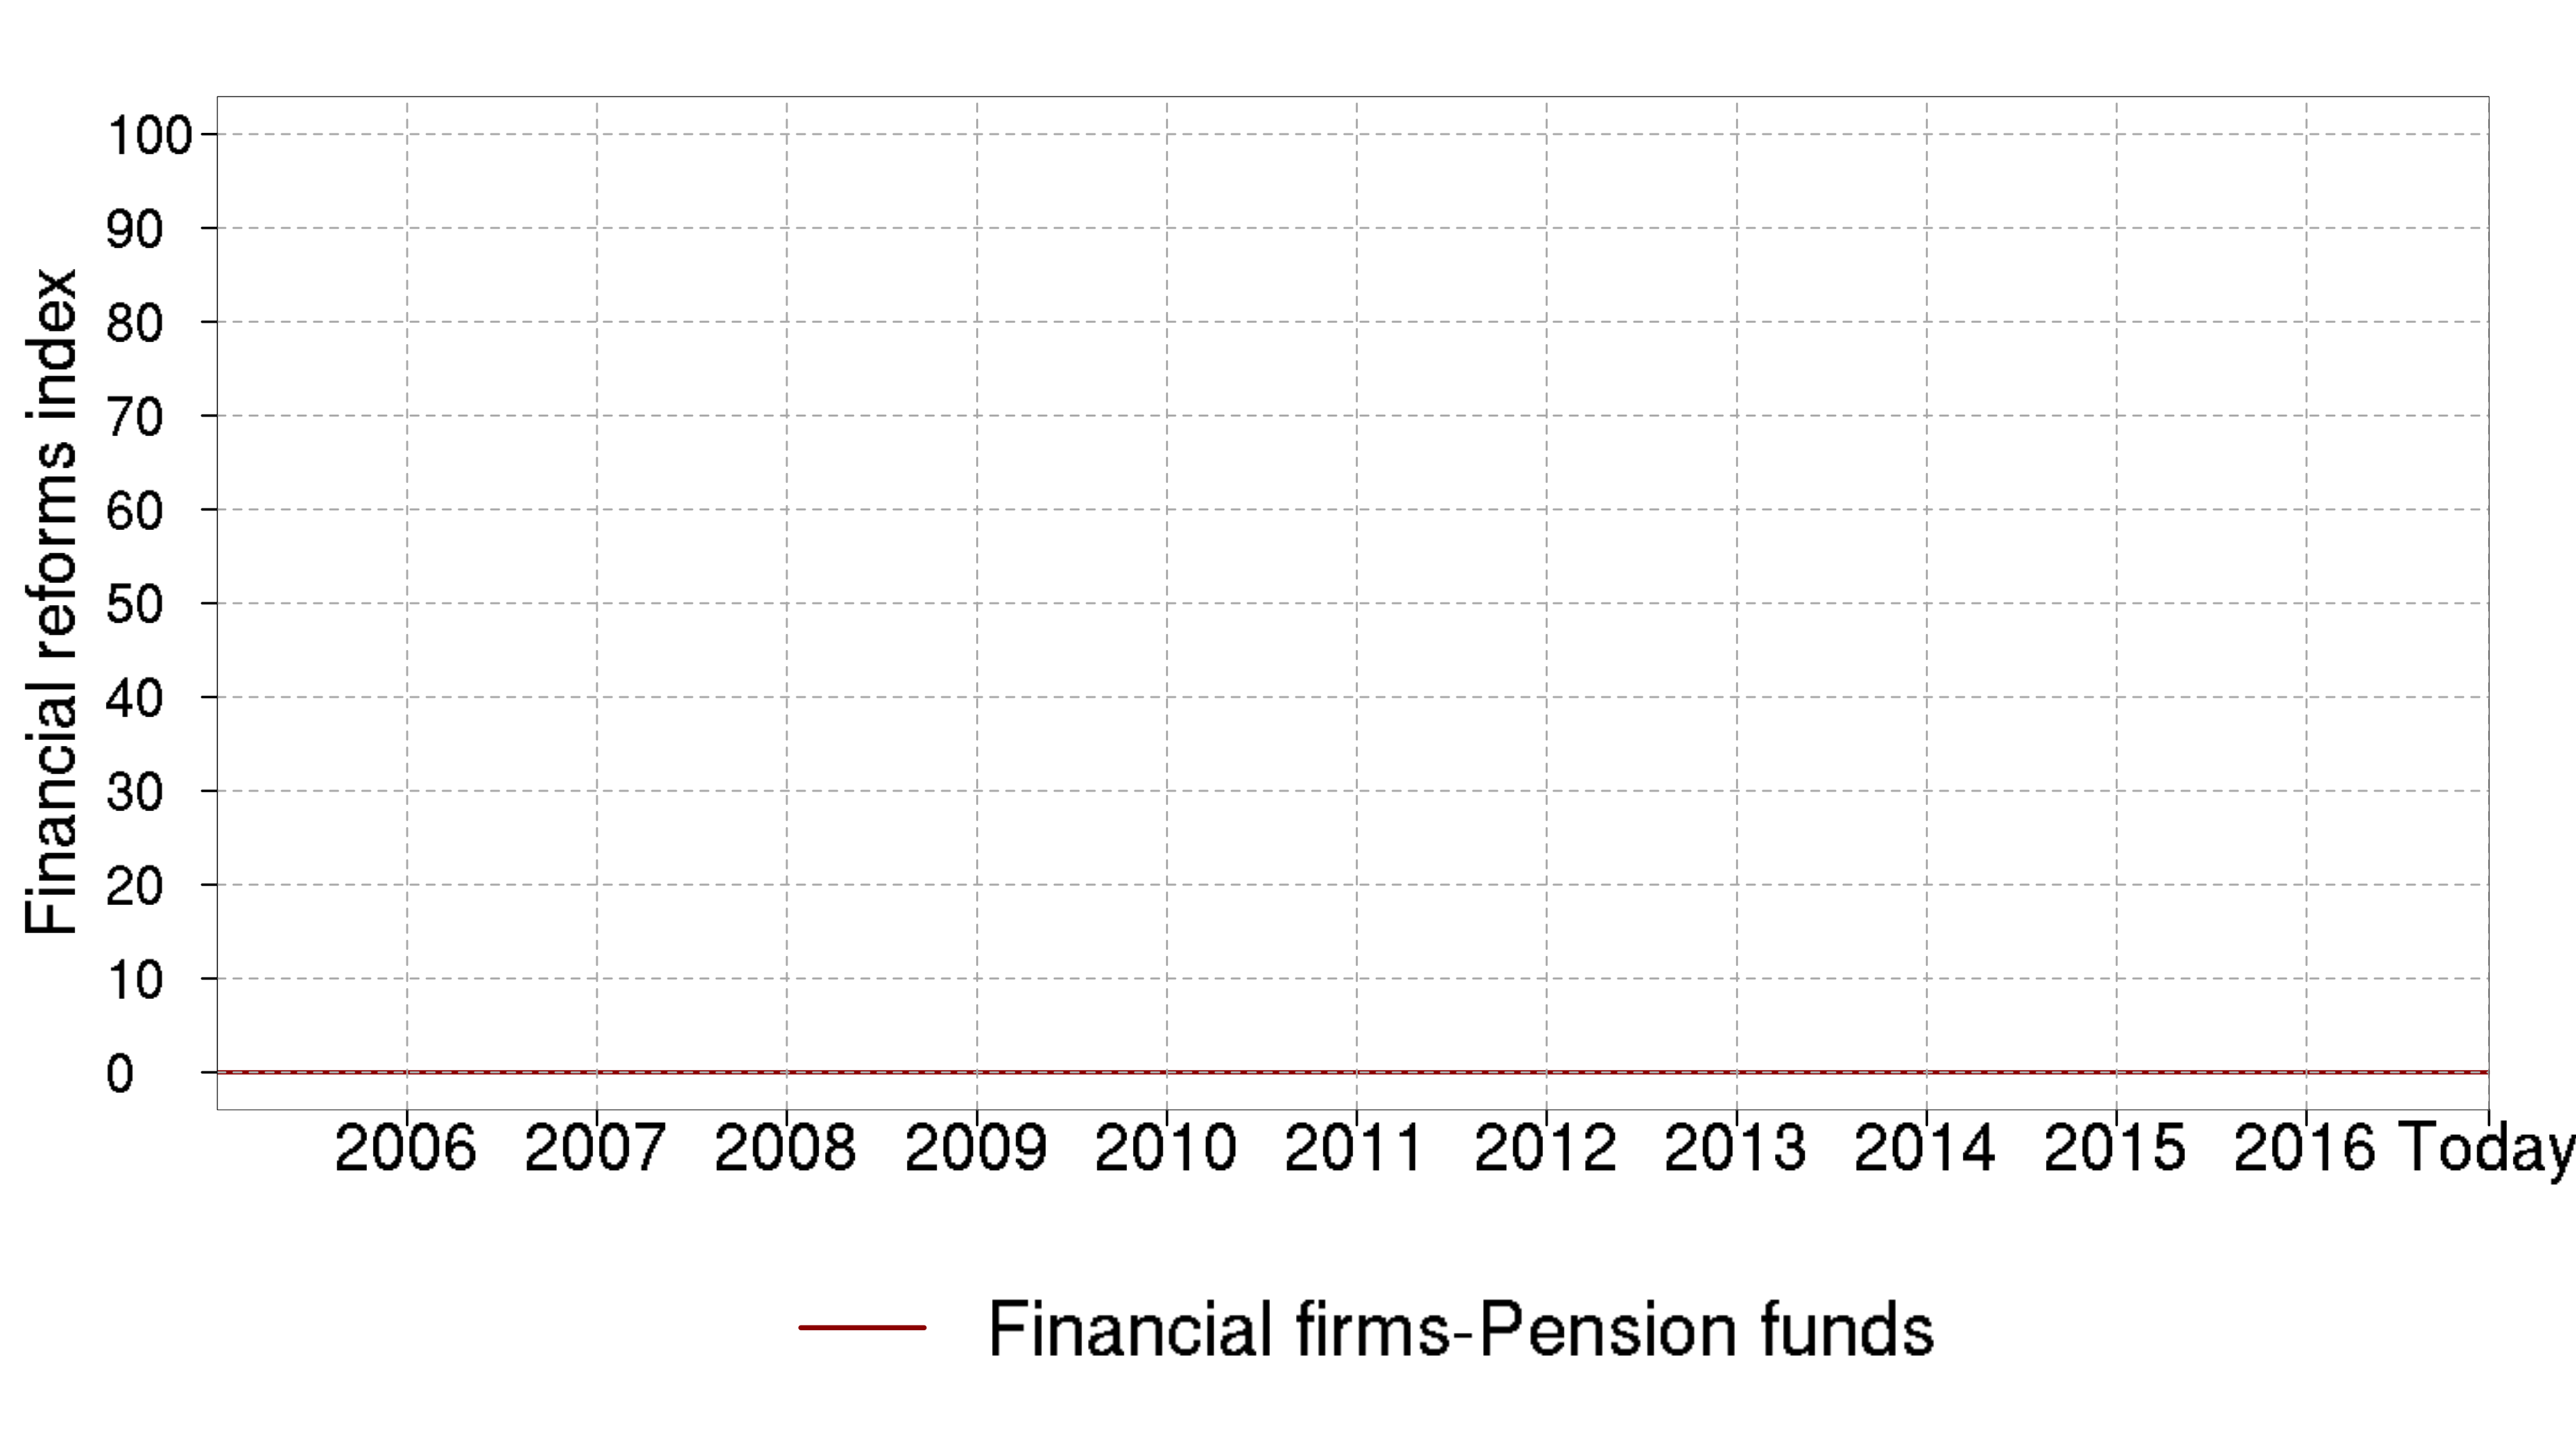
\includegraphics[width=0.65\paperwidth,height=0.45\paperwidth]{../GRAPHS/frm_index_financial_firms_pension_funds.png}
\end{figure}

\begin{titlepage}
  \vspace*{\stretch{1}}

  \parbox{\textwidthorig}{
  \hrule
  \vspace{\baselineskip} \center{\Large Section index: Financial firms}
  \vspace{\baselineskip}
  \hrule
  }
  \vspace{\stretch{1}}

  \parbox{\textwidthorig}{
}
\end{titlepage}

\begin{table} [H]
  \caption{Section index: Financial firms}
  \begin{threeparttable}
    \begin{footnotesize}
      \resizebox{1\textwidth}{!}{
        \begin{tabular} {FGH}
          \multicolumn{3}{p{7in}}{\textbf{\small{Markets:}}} \\ \hline
          \textbf{Section} & \textbf{Subsection} & \textbf{Score} \\ \hline
          \input{../TABLES/frm_index_financial_firms.tex}
          \hline
          \noalign{\vskip .01in}
          \multicolumn{3}{p{6in}}{\textit{\scriptsize{Explanation:
          Subsection-wise scores standing on \today{}.}}}
        \end{tabular}
        
      }
    \end{footnotesize}
  \end{threeparttable}
\end{table}

\begin{figure}[H]
\caption{Section index: Financial firms}
\centering
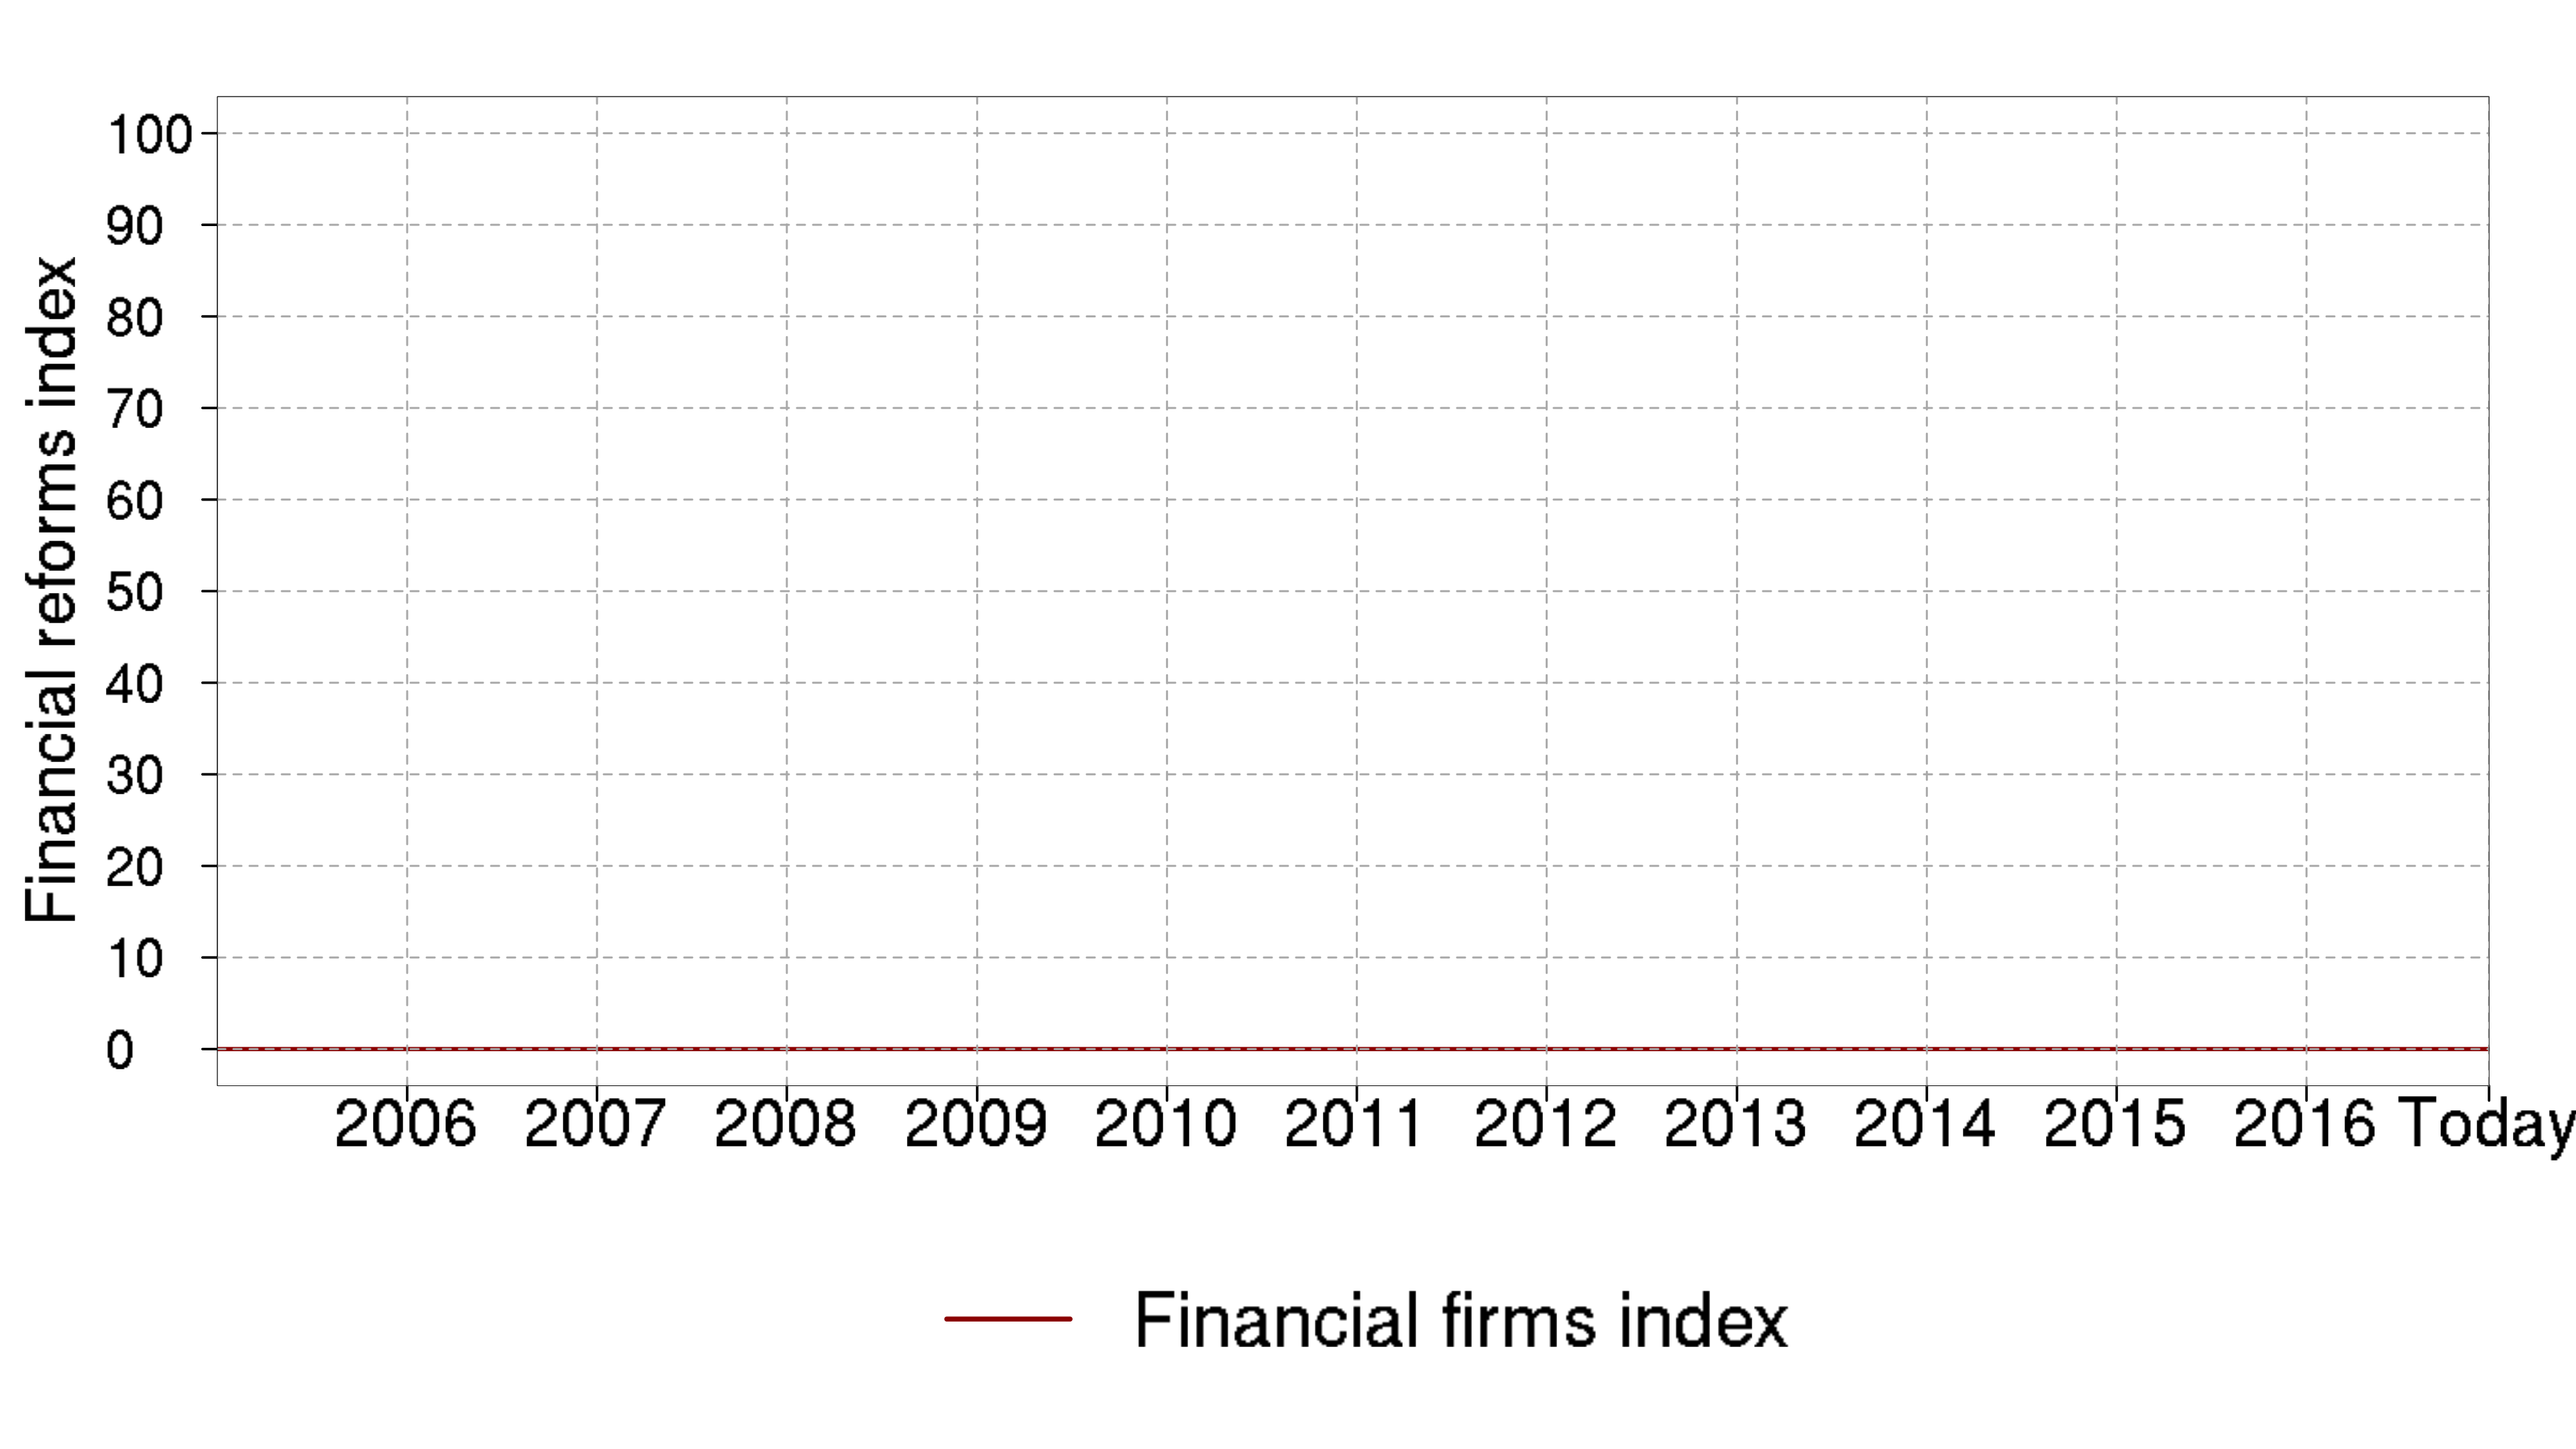
\includegraphics[width=0.9\paperwidth,height=0.7\paperwidth]{../GRAPHS/frm_index_financial_firms.png}
\end{figure}
  

\begin{titlepage}
  \vspace*{\stretch{1}}

  \parbox{\textwidthorig}{
  \hrule
  \vspace{\baselineskip} \center{\Large Overall financial reforms index}
  \vspace{\baselineskip}
  \hrule
  }
  \vspace{\stretch{1}}

  \parbox{\textwidthorig}{
}
\end{titlepage}

\newpage
\refstepcounter{section}
\sectionmark{Overall financial reforms index}
\addcontentsline{toc}{section}{\protect\numberline{\thesection}Overall financial reforms index}

\begin{figure}[H]
\caption{Overall financial reforms index}
\centering
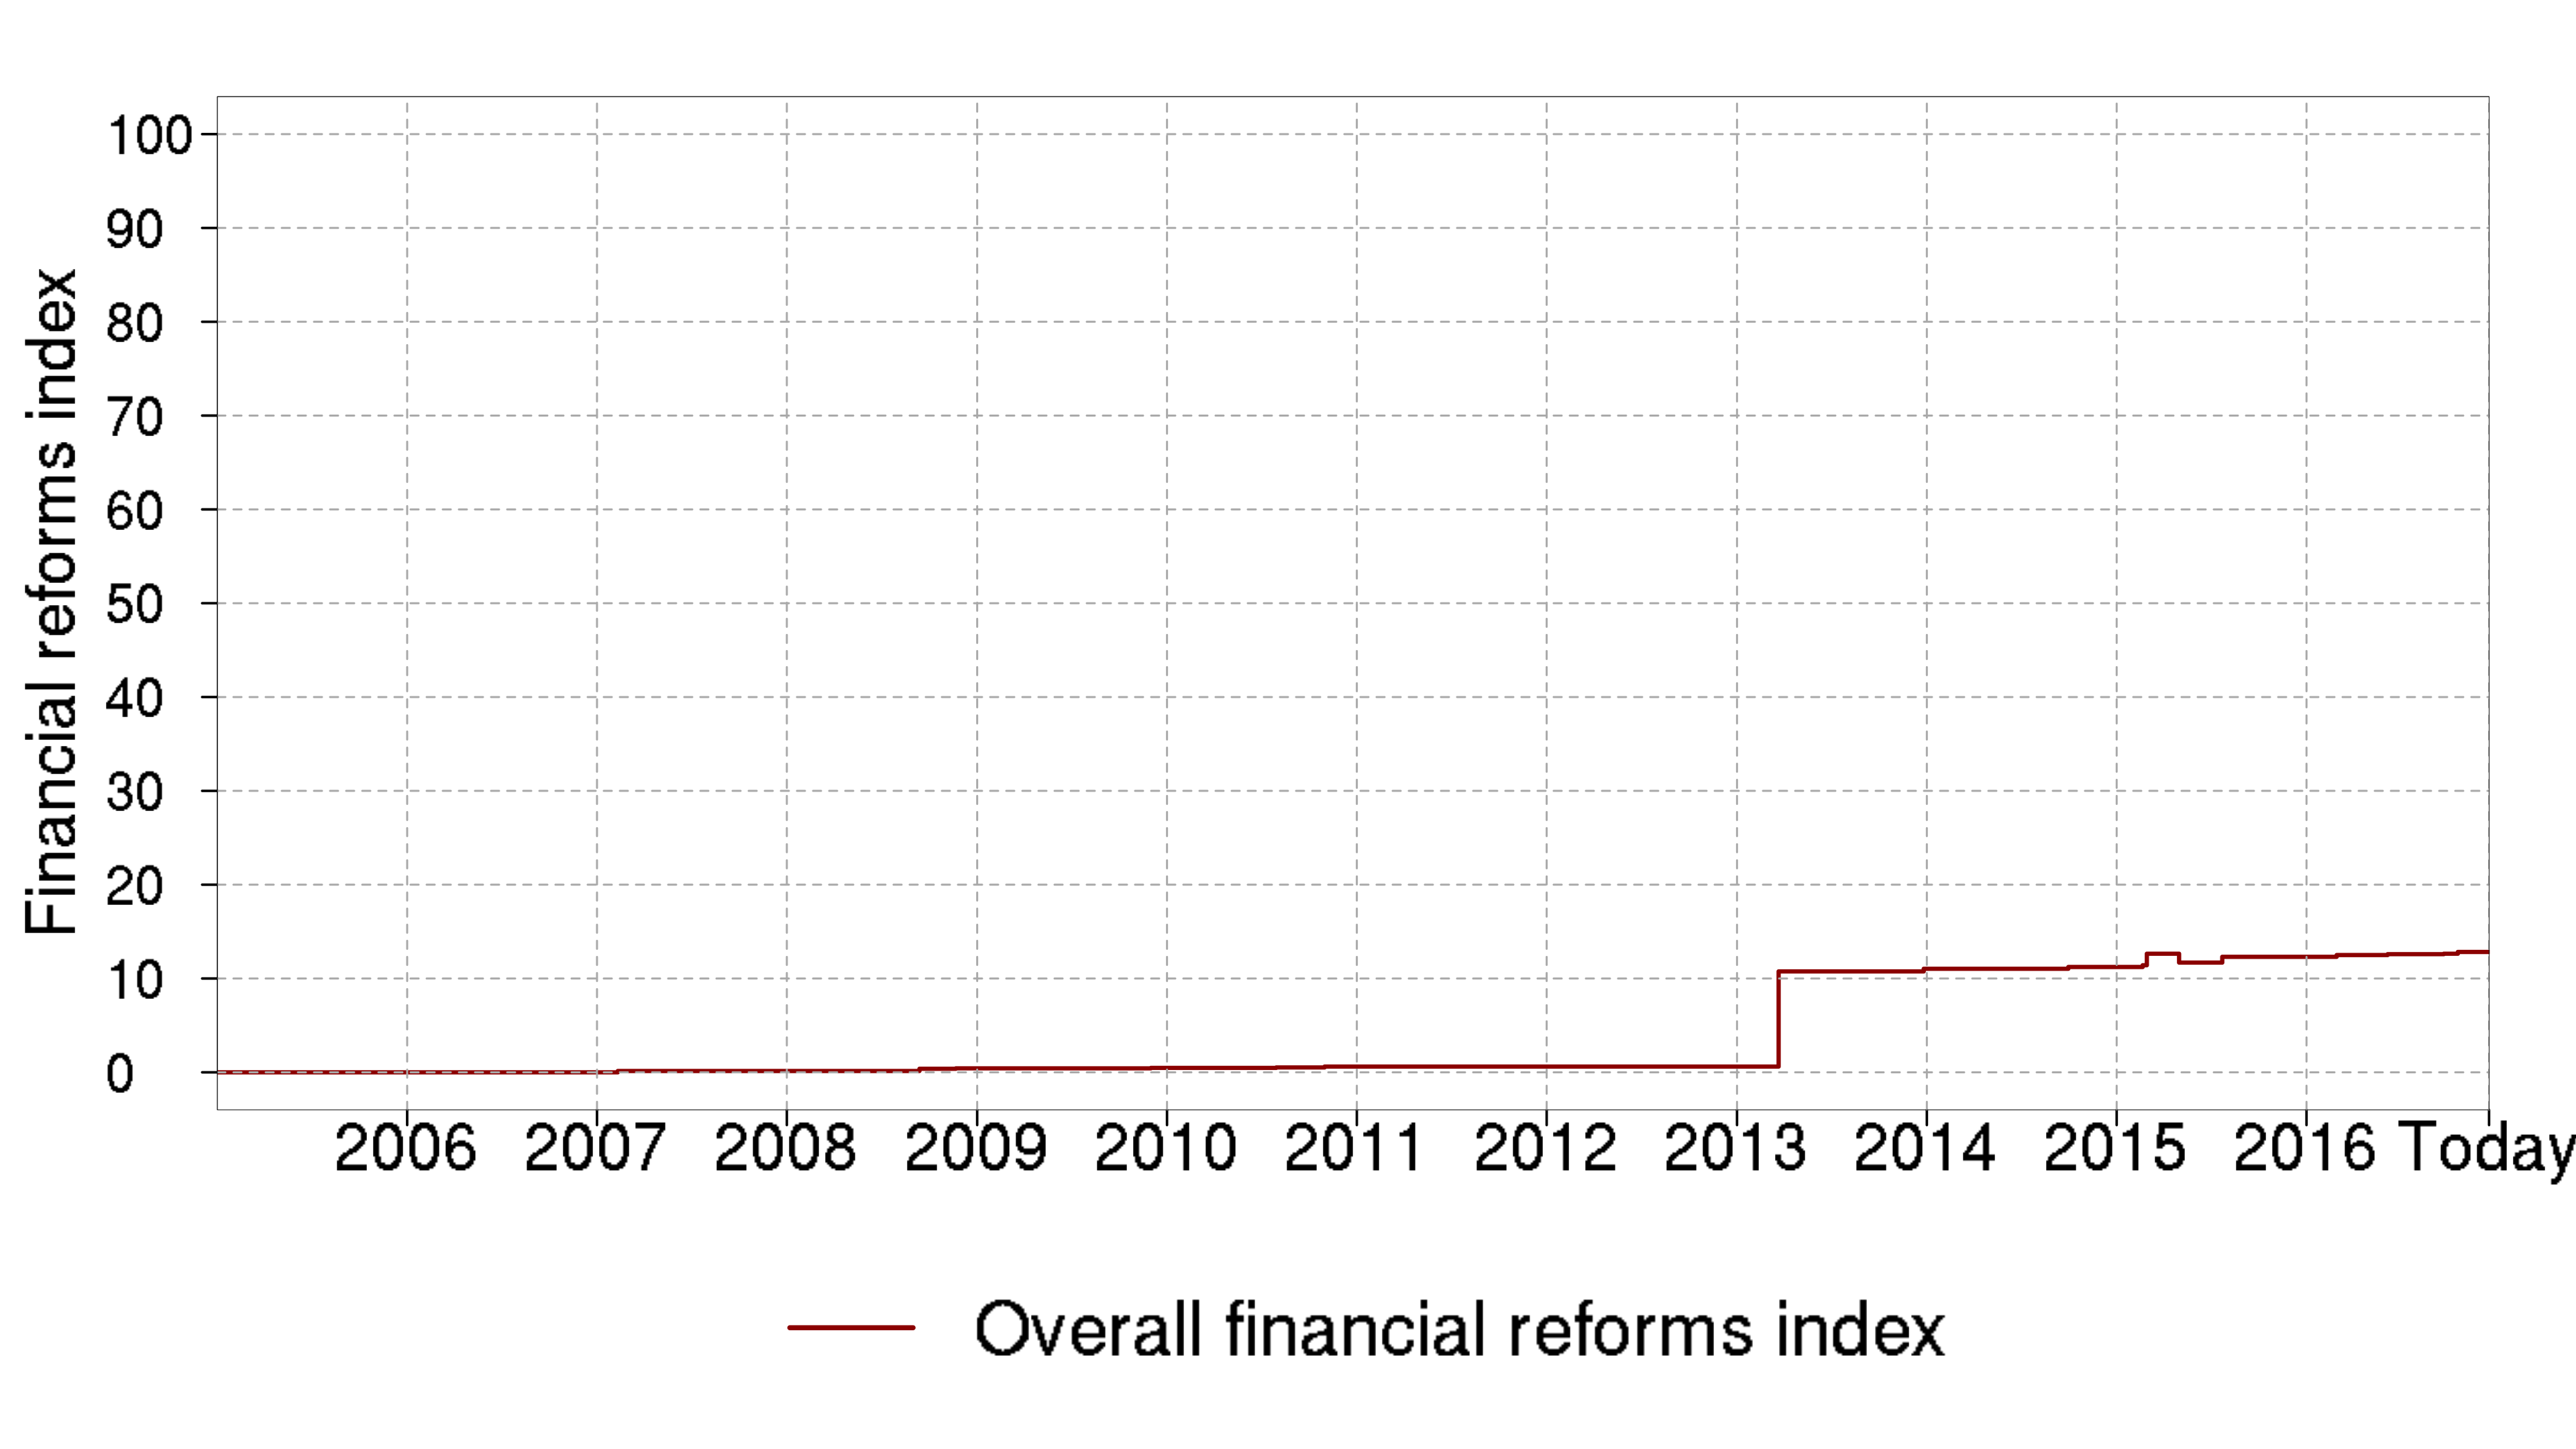
\includegraphics[width=0.9\paperwidth,height=0.7\paperwidth]{../GRAPHS/frm_index_financial_reforms_index.png}
\end{figure}

  
\end{document}
